% !TEX root = ../main.tex
\chapter{绪论} 
\label{chapter:Introduction}

\section{模板概述}
本模板基本结构如下:

\begin{itemize}
\item main.tex: 主文件, 编译对象.
\item figures: 存放论文使用的图片文件夹, 支持多种格式, 直接插入文件名, 不需要输入路径.
\item reference: 存放参考文献文件的文件夹, 默认为bib文件, 可用bibtex编译得到参考文献.
\item style: 学位论文样式文件夹, 定义了论文的整体样式.
\item chapter: 章节文件夹, 包含
\begin{itemize}
\item 论文基本信息文件(cover.cfg);
\item 自定义命令文件(defcommands.tex);
\item 摘要(abstract.tex);
\item 正文章节(chapter1.tex, chapter2.tex, conclusions.tex, ...);
\item 在读期间发表的文章(publications.tex);
\item 在读期间参与的项目(projects.tex)
\item 致谢(thanks.tex).
\end{itemize}
\end{itemize}

\section{编译方式}
本模板支持Windows/Linux/MacOS全平台编译, 编译方式如下:
\begin{enumerate}
\item 安装texlive最新发行版, 如texlive 2023;
\item 使用xelatex编译一次, 然后使用bibtex编译一次, 最后再次使用xelatex编译两次即可.
\end{enumerate}

\section{双语目录与标题}
有些方向要求论文有英文目录或者图表的标题是双语的, 本模板支持双语标题. 调用命令如下:
\begin{verbatim}
\bichapter{中文章节名}{English Chapter Name}
\end{verbatim}
此外, 类似的命令还有: 
\begin{itemize}
\item \verb|\bisection{中文名}{English Name}|
\item \verb|\bisubsection{中文名}{English Name}|
\item \verb|\bisubsubsection{中文名}{English Name}|
\item \verb|\bicaption{中文名}{English Name}|
\end{itemize}

为了生成双语目录, 需要在main.tex中取消\verb|\tableofengcontents|的注释.

\section{算法伪代码}
本模板已引入算法相关宏包. 使用方法见下例 \ref{alg:test}.
\begin{verbatim}
    \begin{algorithm}%[htbp]
        \caption{这是标题}
        \label{alg:test}
        \begin{algorithmic}[1] %每行显示行号
            \Require 这是输入;
            \Ensure 这是输出.
            \For{$j\leftarrow 0,\cdots, d$}
                \State {Test!} \Comment {这里是注释}
            \EndFor
            \If {$w>1$}
                \State {This is a test!}
            \EndIf
            \While {$a>1$}
                \State {Test!}
            \EndWhile
            \State {$\textbf{return }$ 0}
        \end{algorithmic}
    \end{algorithm}
\end{verbatim}

效果如下:
\begin{algorithm}%[htbp]
    \caption{这是标题}
    \label{alg:test}
    \begin{algorithmic}[1] %每行显示行号
        \Require 这是输入;
        \Ensure 这是输出.
        \For{$j\leftarrow 0,\cdots, d$}
            \State {Test!} \Comment {这里是注释}
        \EndFor
        \If {$w>1$}
        	\State {This is a test!}
        \EndIf
        \While {$a>1$}
        	\State {Test!}
        \EndWhile
        \State {$\textbf{return }$ 0}
    \end{algorithmic}
\end{algorithm}


\section{插图与引用}
如图 \ref{fig:logo}.
\begin{figure}[h]
	\centering
	
\includegraphics[scale=0.25]{logo}
	\bicaption{广州大学Logo}{GZHU LOGO}
	\label{fig:logo}
\end{figure}

如果要生成图表的标题目录, 需要在main.tex文件中取消以下两行的注释:
\begin{verbatim}
\listoftables               % 表格目录
\listoffigures              % 插图目录
\end{verbatim}

\section{引用参考文献}
本模板使用bib文件作为参考文献文件, 同时引入了natbib宏包, 此外增添了两个自定义命令:
\begin{itemize}
\item \verb|\citeyearn{citekey}|  ~  引用年份时可在年份后面自动添加``年''
\item \verb|\upcite{citekey}| ~ 上标引用.
\end{itemize}

这是一句测试\cite{Hazay_2010_Efficient}. 引用年份时: \citeyearn{Hazay_2010_Efficient}. 上标引用\upcite{Hazay_2010_Efficient}.

\section{常见问题}
Q1: 如何添加更多章节文件?\\
A1: 按如下步骤操作:
\begin{enumerate}
\item 在chapter文件夹下添加新的tex文件, 例如chapter3.tex
\item 打开main.tex, 在第100行后添加\verb|% !TEX root = ../main.tex
\chapter{多模态脑影像的智能辅助融合} 
\label{chapter:multiFusion}
%不同疾病依赖的影像检查类别不同,本文工作主要关注脑疾病的诊断,脑疾病种类繁多,诊断过程复杂,因此需要多模态影像技术共同作为辅助诊断依据,以提高诊断的准确性和全面性。
不同疾病依赖的影像检查类别不同,不同的影像在揭示不同脑部病变的特异性表现上具有不可替代的价值。本文的工作聚焦于脑部疾病这一多元且复杂的诊断领域,鉴于其多样化的病理类型与诊断挑战,单一影像技术往往不足以实现精确诊断。因此,核心探讨的是如何有效地整合运用多种影像模态,旨在最大程度地提升脑疾病诊断的精确度与完整性。
%随着影像处理技术的不断成熟和进步,影像融合技术正逐渐成为众多研究领域的瞩目焦点,其中医学影像融合技术的崛起更是为医疗领域带来了全新的可能性。
在这一章中,提出了两种针对多模态医学影像融合算法。一种是医学语义引导的脑影像融合双分支网络(MsgFusion)\cite{wen2023msgfusion},另外一种是多维特征自适应线性融合网络(MdAFuse)\cite{wen2024tip},分别于\ref{chapter3.1:MsgFusion}和\ref{chapter3.2:MdAFuse}小节详细介绍。

\section{基于脑影像的临床语义引导融合}\label{chapter3.1:MsgFusion}
%多模态影像融合在医学影像分析和应用中起着至关重要的作用,其中计算机断层扫描(CT)、磁共振(MRI)、单光子发射计算机断层扫描(SPECT)和正电子发射断层扫描(PET)是常用的模态,特别是用于脑部疾病的诊断。现有的融合方法大多没有考虑医学影像的特点,采用与自然影像相似的融合策略和评价标准。虽然独特的医学语义信息隐藏在不同的模态中,最终的临床评估的融合结果被忽略。因此我们提出一种医学语义引导的融合方法(MsgFusion)。首先在MRI/CT/PET/SPECT影像的关键MS-Info和影像特征之间建立关系,以指导使用两个分支的特征提取和影像融合框架的设计。并使用一种基于分层分类的融合策略,用于重建融合影像,以保持和增强反映解剖结构和功能代谢的突出医学语义信息。对多对MRI-PET/SPECT和MRI-CT影像进行了融合实验。通过7种经典客观质量评价和1种对30名临床医生的主观临床质量评价,MsgFusion的融合结果优于现有的代表性方法。
%我们已在GitHub上分享了该方法的源代码(https://github.com/22385wjy/MsgFusion)。

\subsection{引言}
自20世纪90年代以来,影像融合技术在医学领域得到了发展和应用。然而,自然图像和医学影像之间存在许多差异,例如信噪比、分辨率、相关区域大小和影像场景\cite{wei2022beyond,shen2021Interpretable,guo2018single,xia2019global}。直接将传统的自然影像网络应用于医学影像往往效率低下,因为这会导致性能下降。因此,本节认为有必要深入分析医学影像的特点,设计一个专用的网络模型。医学影像融合可以方便医生对病例进行观察、评估和对病变进行分析,从而做出更准确的诊断。一般来说,CT/MRI/SPECT/PET常被医生用来观察脑部疾病。不同的医学影像模态具有独特的医学语义信息(medical semantic information,MS-Info)。不同模态的融合结果应该保持并增强相关MS-Info在每个模态中对诊断有意义。因此,本节提出了一个医学语义引导的双分支网络。在特征提取阶段,根据不同模态的MS-Info引导影像特征,采用有利于提取相应影像特征的网络分支策略,保证融合结果中各模态的MS-Info得到保持和增强。影像融合技术将两幅源影像中的这些信息融合并增强到一幅影像中,使医生能够更方便、更准确地观察、理解和诊断疾病。因此,脑CT/MRI/SPECT/PET影像的融合技术对帮助医生诊断脑部疾病具有重要意义。

近年来,许多医学影像融合方法被提出。这些现有的方法主要包括两类,即,传统的人工融合方法\cite{2017Boundary,2018Multi,2018Infrared,2020An,diwakar2021multi,2020Latent}和基于深度学习的融合方法\cite{2018DenseFuse,2018Deep,2018Unsupervised,kumar2019structural,2019FusionGAN,2020IFCNN,2020NestFuse,2020FusionDN,zhao2021learning}。传统的方法是由人工认知驱动的。传统的特征提取方法主要依靠人工提取,需要专业的领域知识和复杂的参数调整过程。此外,每种方法都针对特定的应用场景。基于深度学习的方法是数据驱动的。它们可以通过学习大量的样本来获得深度抽象的特征。数据集的表达更加高效和准确,提取的抽象特征展现出较高的稳健性和广泛的适用性。目前,DL方法已成功应用于影像处理的许多领域。然而,基于DL的医学影像分析仍处于早期发展阶段。相关的研究正成为热点,具有广泛的应用前景。本文提出了一种新的CT/MRI/SPECT/PET脑影像融合方法,目的是保留和增强原始影像中重要的MS-Info信息,以辅助医生诊断脑部疾病。
本节工作作出了以下贡献:

\begin{itemize}
    \item 这是第一个关注多模态医学影像MS-Info的影像融合工作,并将其映射到相应的影像特征上。设计了一种医学语义引导的双分支网络,以有效地学习与不同模态(MRI/PET/SPECT/CT)的MS-Info对应的深度特征。
    \item 在SF-Branch中,本节提出了一种空间域和频域相结合的特征提取方案,在保留原始影像信息的基础上,更方便地从MRI中提取关键MS-Info的相应特征,这在医学影像融合的智能辅助设计中尚属首次。
    \item 在GV-Branch中,本节提出了一种结合灰度空间和改进的HSV颜色空间中的亮度分量信息的特征提取方案,提取对应于PET/SPECT影像的关键MS-Info的基础上,保留原始影像信息的深层次特征。
    \item 本节提出了一个新的临床评估,其是来自医生的评价。他们评估融合影像的质量取决于有多少MS-Info从源影像中被保留和增强。同时,本研究采用了七种常见的客观评价指标。实验结果表明,在所有评价指标结果中,所提出的影像融合方法均优于9种有代表性的融合方法。
\end{itemize}


\subsection{相关工作}
现有的融合技术涵盖了传统的和以深度学习为基础的各类方法。在这一部分中,本节主要介绍了医学影像融合的相关工作,影像处理中的傅里叶变换和HSV颜色空间变换的理论。

\subsubsection{医学影像融合}
医学影像具有自身的特殊性,医学影像融合在影像引导的医学诊断、治疗等计算机视觉任务中发挥着重要作用。其中,多模态影像融合模块也被设计用于疾病辅助诊断,如\cite{2019Inter}。Algarni提出了一种基于多模态影像融合的诊断系统,适用于融合MRI和CT影像\cite{2020Automated},但仅适用于融合MRI和CT影像。为了开发一种即使受损影像也能准确保留细节信息的融合方法,Li等人将低秩稀疏矩阵字典学习方法应用于医学影像融合\cite{Li2018Joint},可以同时达到去噪和增强的效果。Panigrahy等人提出了一种利用双通道PCNN的医学影像融合方法(WPADCPCNN)\cite{panigrahy2020mri},该方法可以获得良好的融合效果,但仅适用于MRI-SPECT融合。Parvathy提出了一种基于优化阈值和深度学习的融合模型\cite{2020A},可以为专家提供解剖和生理数据,以促进诊断过程。针对彩色空间域的伪彩色影像,提出了一种基于Otsu自适应阈值(atsIF)的双尺度影像融合方法\cite{2020An}。

Hermessi等人提出了一种基于卷积神经网络相似性学习的多模态MRI和CT影像融合方法\cite{2018Convolutional}。Das等人提出了一种新的基于低秩纹理先验分解和超像素分割的影像融合\cite{das2022optimized},该方法结合了三种方案,即,采用灰度优化、优化的低秩纹理先验知识和像素相关的高斯混合模型,有效地提高了融合影像的视觉保真度。Kumar等人提出了一种新的CNN方法,专门用于MRI和PET影像融合\cite{kumar2019structural},并在训练过程中使用结构相似性指数(SSIM)作为损失函数。Liang等人提出了多层级联融合网络(MCFNet)\cite{2019MCFNet}。该网络补充了融合医学影像在两次下采样过程中丢失的空间信息。Yu等人提出了网络(IFCNN)\cite{2020IFCNN},Li等人提出了通用网络(NestFuse)\cite{2020NestFuse}。这两种方法均采用卷积神经网络进行特征提取,然后采用特征值最大化策略进行多模态医学影像融合。它们可以获得很好的融合效果,但由于卷积网络不能捕捉长距离的相关性,无法避免全局纹理信息的丢失。

目前,大多数医学影像融合方法都有局限性。首先,MRI/CT/PET/SPECT是常用的脑成像技术,然而,在大多数医学影像融合方法中仅考虑两种模态。其次,大多数方法主要遵循自然图像融合的思想。事实上,医学影像与自然图像之间存在差异,不同模态的医学影像之间也存在很大差异。没有充分考虑不同模式的关键MS-Info。第三,现有方法的融合策略采用加权求和策略和最大值策略。权重系数的选取需要经过多次试验,由结果来确定。求和策略会导致融合影像模糊,而最大值策略会丢失一些关键特征。这种简单、单一的融合策略会导致源影像中关键MS-Info的丢失。第四,医学影像融合的最终目的是方便临床医生阅读,融合影像的质量会影响医生对疾病的诊断。因此,临床医生的质量评估应当是金标准。现有的医学影像融合方法很少考虑临床医生的评价。最主要的一点是没有充分考虑源影像的MS-Info。因此,本文构建了一种新的融合网络,重点是脑医学影像的MS-Info和临床评价的融合目标。


\subsubsection{频域变换在影像处理中的应用}
在图像处理的过程中,要将图像转换到频域进行处理,常用的是傅立叶变换。在图像处理领域,可以利用傅立叶变换来获得空间图像的频率分布,然后在频域进行各种图像处理,可以有目的地实现许多功能。近年来,傅立叶变换在图像编码\cite{abiko2019image}、图像检测\cite{kuo2020fast}、图像压缩\cite{bag2021lossy}、图像分析\cite{2012Joint,2020Joint}、图像配准\cite{atta2018joint}和图像重建\cite{pezzotti2017Efficient}中有着广泛的应用。傅里叶变换在图像融合中具有潜在的优势。Naidu等人\cite{Naidu2011Multi}提出了一种基于快速傅立叶变换(MFFT)的多分辨率图像像素级融合算法。然而,这种方法是基于多分辨率自然图像的融合。据广泛阅读文献发现,目前还没有利用傅立叶变换进行医学影像融合的案例。此外,频域分析方法在基于深度学习的方法中也具有不可否认的潜力。例如,Kai等人\cite{xu2020learning}提出了一种基于频率的学习方法,证明了频域学习方法在分类、检测和分割任务中的普遍性和优越性。在频域对影像进行处理,可有效地保存影像信息,提高精度。因此,本节也采用频域处理对医学影像进行处理,并联合深度学习方法,以达到更好的融合效果。

在数字图像处理技术中,傅立叶变换占据着至关重要的地位,它可以将图像从空间域变换到频率域。从本质上讲,变换后的图像与原始图像相同,并且可以更直观地分析图像的幅度和相位分量,即图像的全局和局部信息。这些信息对于MRI的全局纹理和局部几何形状都是非常重要的信息,代表了软组织边缘和内部结构的语义特征。利用傅立叶变换对MRI进行处理,对融合后的病灶定位起着关键作用。

%\if 0
\subsubsection{彩色空间变换在影像处理中的应用}
RGB、YUV和HSV颜色空间通常用于影像处理。RGB颜色空间是最常用的影像颜色表示空间。YUV易于压缩,便于传输和处理。HSV颜色空间最适合人类的视觉感知,因为在该空间中的颜色变化很容易被人类区分。H(Hue)表示色调,指影像的颜色偏好,S(Saturation)表示颜色的强度或纯度。V(Value)表示颜色的亮度。RGB和HSV转换通常用于影像处理以增强影像\cite{peng2018multi}。(R,G,B)分别是颜色的红色、绿色和蓝色坐标,其值是0和1之间的真实的数。如果M等于R、G和B中的最大值,并且m等于这些值中的最小值,则RGB和HSV之间的转换过程如等式(\ref{Hcomponent})所示:


\begin{equation}\label{Hcomponent}
\begin{aligned}
&H= \begin{cases}0^{\circ} & \text { if } M=m \\
60^{\circ} \times \frac{G-B}{M-m}+0^{\circ}, & \text { if } M=R \text { and } G \geq B \\
60^{\circ} \times \frac{G-B}{M-m}+360^{\circ}, & \text { if } M=R \text { and } G<B \\
60^{\circ} \times \frac{B-R}{M-m}+120^{\circ}, & \text { if } M=G \\
60^{\circ} \times \frac{R-G}{M-m}+240^{\circ}, & \text { if } M=B\end{cases} \\
&S= \begin{cases}0, & \text { if } M=0 \\
\frac{M-m}{M}=1-\frac{m}{M}, & \text { otherwise }\end{cases} \\
&V=M
\end{aligned}.
\end{equation}

HSV颜色空间相较于RGB颜色空间,在模拟人类视觉感知上更为贴近\cite{jin2018multimodal},HSV颜色空间中多个通道的使用可以单独处理,并且彼此独立。所以,在HSV色彩模式下,能够显著简化影像分析与处理的复杂度。它也用于影像融合\cite{2018Scene}。HSV颜色空间在影像处理中得到了广泛的应用,通常使用不同的通道来解决不同的问题。与RGB空间相比,HSV空间可以非常直观地表达颜色、色调和明暗度,便于颜色之间的对比和情感的交流。因此,本文还将HSV颜色空间的优势应用到医学影像融合中。为了更好地提取有用的MS-Info,本节采用了一个自定义的$V$分量,这将在下一节中详细介绍。
%\fi


\if 0
\begin{table*}[htb]
\centering
\caption{MRI/CT/PET/SPECT的关键医学语义信息如何引导MsgFusion两个分支的设计}\label{semanticfeature}
\renewcommand\arraystretch{1.5}
%\begin{tabular}{|c|c|c|c|c|}
\begin{tabular}{|p{42pt}<{\centering}|p{80pt}<{\centering}|p{80pt}<{\centering}|p{80pt}<{\centering}|p{50pt}<{\centering}|}
\hline
Modality & \textbf{Key MS-Info} & \textbf{Image Feature}  & \textbf{Extraction Strategy}  & \textbf{Branch}\\ \hline
\multirow{4}{*}{\begin{tabular}[c]{@{}c@{}}\textbf{MRI}\\
\begin{minipage}{0.09\textwidth}
\centering
      \includegraphics[width=13mm, height=13mm]{figs/013MRI}
\end{minipage}
\end{tabular}}

& Clear shape of soft tissue
& Boundary zone

& High frequency band in Frequency Domain
& \multirow{3}{*}{\begin{tabular}[c]{@{}c@{}} \\SF-branch\end{tabular}} \\ \cline{2-4}
& Clear internal structure of soft tissue
& Internal texture detail
& Low frequency band in Frequency Domain  & \\ \cline{2-4}
& NIL
& More source image information
& Spatial Domain &  \\ \hline

\multirow{2}{*}{\begin{tabular}[c]{@{}c@{}}\textbf{CT}\\
\begin{minipage}{0.09\textwidth}
\centering
      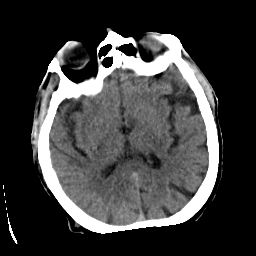
\includegraphics[width=13mm, height=13mm]{figs/013ct}
\end{minipage}
\end{tabular}}
& High-resolution global anatomical structure  of hard tissue
&\multirow{5}{*}{\begin{tabular}[c]{@{}c@{}}Global contour\\  lines; Local \\shape location \\of tiny area;\\More source \\image informat-\\ion\end{tabular}}
& \multirow{5}{*}{\begin{tabular}[c]{@{}c@{}}  Multi-scale; \\ Concatenate;\\
Gray color space\end{tabular}}
& \multirow{3}{*}{\begin{tabular}[c]{@{}c@{}} \\\\\\ GV-branch\end{tabular}}\\  \cline{2-2}
& High-resolution local anatomical  structure of hard tissue
& &  &    \\ \cline{1-2}

\multirow{2}{*}{\begin{tabular}[c]{@{}c@{}}\textbf{PET}\\
\begin{minipage}{0.09\textwidth}
\centering
      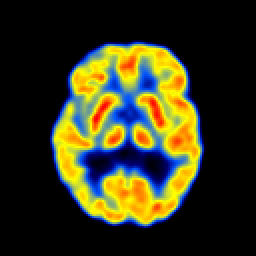
\includegraphics[width=13mm, height=13mm]{figs/013pet}
\end{minipage}
\end{tabular}}
& Obvious display of early small lesion
& &  &  \\ \cline{2-4}
& High-distinguished functional-metabolic abnormity tissue
& Brightness
& Brightness component of HSV color space & \\ \hline
\end{tabular}
\end{table*}
\fi
    \begin{figure*}[htb]
      \centering
          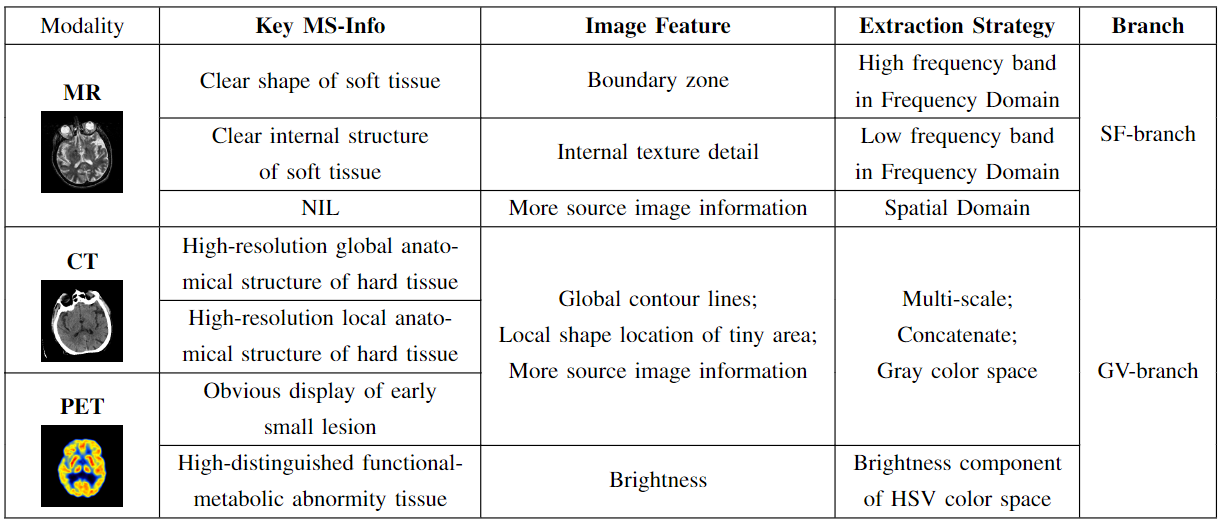
\includegraphics[width=0.9\columnwidth]{figs/paper1semanticfeature.png}
          \caption{多模态医学影像的关键医学语义信息引导两个特征提取分支的设计}\label{paper1semanticfeature}
     \end{figure*}
    
\subsection{医学语义引导的双分支网络}
不同模态的医学影像中包含着不同的医学语义信息(medical semantic information,MS-Info),这对临床疾病诊断具有重要意义。因此,应该保持和加强各自在其多模态医学影像融合结果的MS-Info。为了实现这一目标,本节首先根据临床医学和成像理论分析每种模态的MS-Info。然后,映射关键MS-Info到影像特征,并为不同的功能设计有效的提取策略。MRI/CT/PET/SPECT的关键医学语义信息如何指导MsgFusion的两个分支设计的细节在表\ref{paper1semanticfeature}中给出,其引导构建所提出的医学语义引导的双分支融合网络(Medical Semantic Guided Fusion,MsgFusion)的两个分支。

 \begin{figure*}[htb]
  \centering  %width=\columnwidth width=\textwidth
      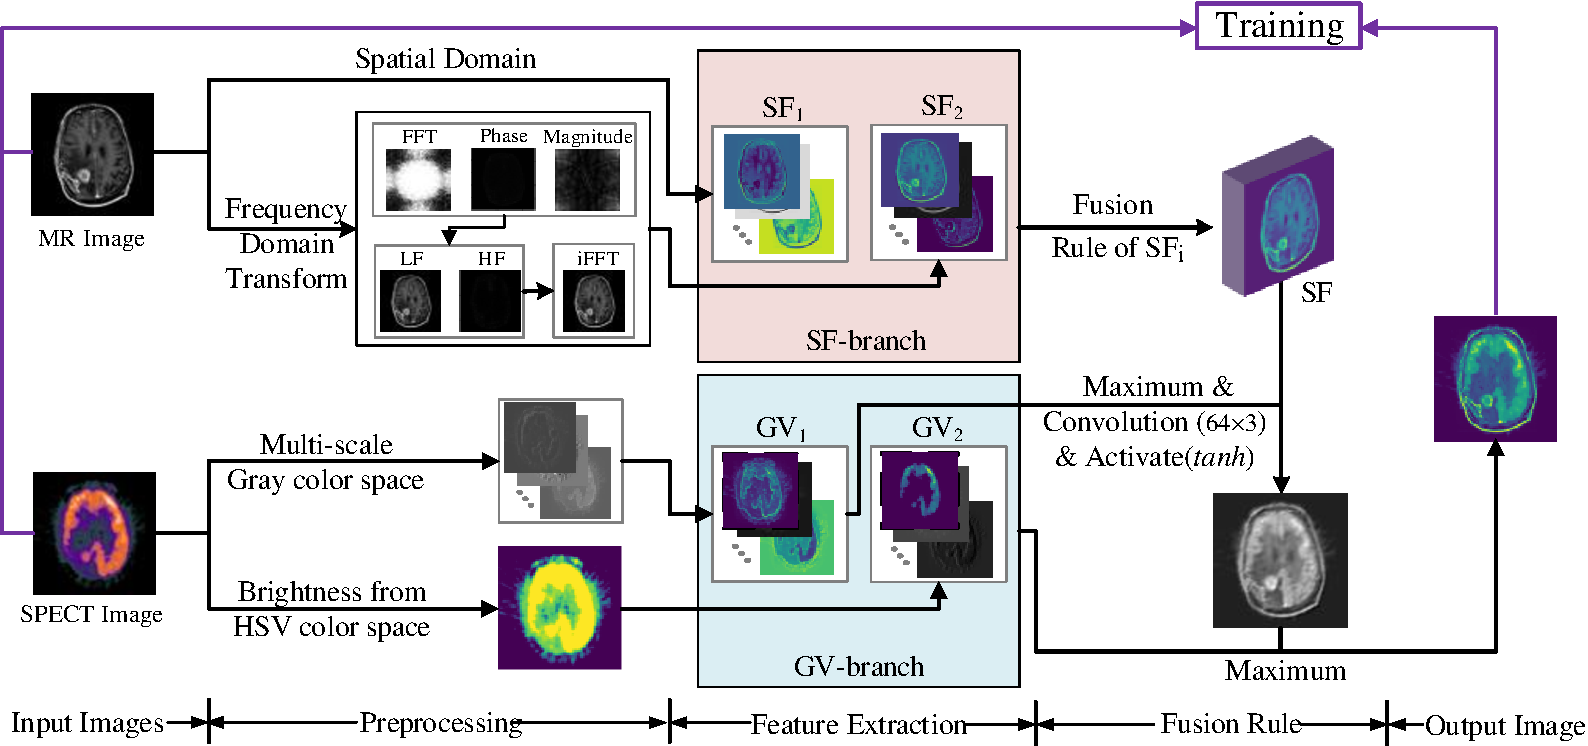
\includegraphics[width=0.9\textwidth]{figs/paper1framework_20221225.pdf}
      \caption{MsgFusion方法的框架:医学语义引导的多模态脑影像融合双分支网络}
      \label{paper1Framework}
 \end{figure*}
 
MsgFusion的整体框架如图\ref{paper1Framework}所示,其中预处理和特征提取是关键步骤。首先,在深度MS-Info提取阶段,网络结合了两个特征提取分支,空间域和频率域结合的分支(the branch combines spatial domain and frequency domain,SF-Branch)和灰度与自定义V分量结合的分支(the branch combines gray color space
and self-defined brightness information,GV-Branch),如图\ref{paper1Framework}所示。SF-Branch采用傅立叶变换,GV-Branch采用HSV颜色空间,不仅充分利用了影像的空间和频率关系,而且从影像的重要信息中提取了丰富的语义特征。第二,是本节的分层融合策略。这两个特征提取分支的结合不仅提高了算法的性能,而且有效地获得了多模态医学脑影像的重要的MS-Info。

\subsubsection{空间域和频率域结合的方案}
SF-Branch被设计用于从MRI中提取深度特征。如表\ref{paper1semanticfeature}所示,MRI的MS-Info,即,软组织的清晰形状和内部结构在频域中更容易区分为高频带信息和低频带信息。为了有效地提取MS-Info对应的深层特征和更多的源影像信息,本节采用了频域和空间域相结合的策略。图\ref{paper1AS_Fu}示出了SF-Branch的过程。
    \begin{figure*}[htb]
      \centering
          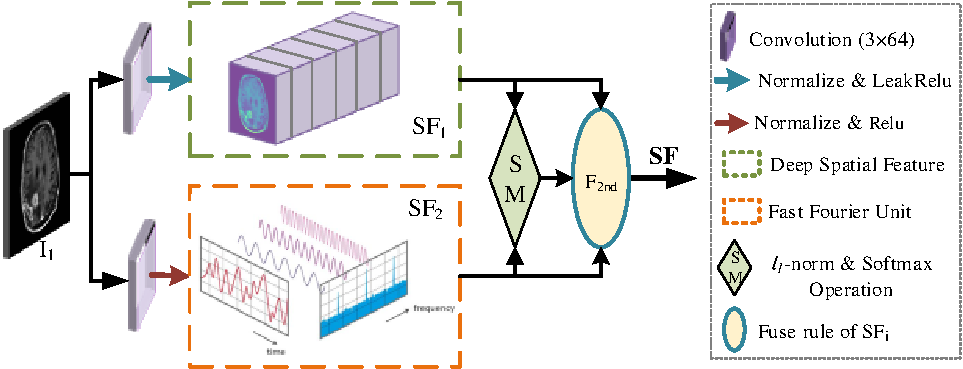
\includegraphics[width=0.9\columnwidth]{figs/paper1AS_Fu.pdf}
          \caption{SF-Branch提取特征的过程}\label{paper1AS_Fu}
     \end{figure*}
     
特征提取的SF-Branch包括两部分,一部分是从神经网络的卷积特性中获取源MRI的深层特征;另一部分是从频域中获取MS-Info对应的特征。在第一部分中,通道被放大到64,卷积核的大小设置为7 × 7,步幅设置为1,填充量为3。批量归一化并使用LeakyReLU(alpha=0.2,inplace=true)激活卷积特征。该部分的输出记录为$SF_1$,如图\ref{paper1AS_Fu}所示。另一部分先采用频域处理,其输出记为$SF_2$。频域处理的示例显示在由图\ref{paper1Framework}中用频域变换标记的箭头所指向的正方形中。具体地,一幅M × N影像的二维离散傅立叶变换和逆变换表示为等式(\ref{ftFunction})和式(\ref{iftFunction})。其中,$x$和$y$为空间域中的影像变量,$f(x,y)$表示点$(x,y)$处的灰度值,$u$和$v$为频率变量,当$u$和$v$为0时,为原点处的傅立叶变换,相当于一幅影像的平均灰度值。

    \begin{equation}\label{ftFunction} %离散傅里叶变换
     F(u,v)=\frac{1}{M N} \sum_{x=0}^{M-1} \sum_{y=0}^{N-1} f(x,y) e^{-j 2 \pi(u x / M+vy / N)}
    \end{equation}
    \begin{equation}\label{iftFunction} %离散傅里叶逆变换
     f(x,y)=\sum_{u=0}^{M-1} \sum_{v=0}^{N-1} F(u,v) e^{j 2 \pi(u x / M+v y / N)}
    \end{equation}

假设$Re$和$Im$分别用于表示$F$的实部的和虚部,则它们的计算是根据等式(\ref{RealPart})和等式(\ref{imaginaryPart}):

    \begin{equation}\label{RealPart}   %实部
      \sum_{x=0}^{N-1} \sum_{x=0}^{N-1} f(x,y) \cos \left(2 \pi\left(\frac{w x}{N}+\frac{v y}{N}\right)\right)
    \end{equation}
    \begin{equation}\label{imaginaryPart}  %虚部
       \sum_{x=0}^{N-1} \sum_{y=0}^{N-1} f(x,y) \sin \left(2 \pi\left(\frac{w x}{N}+\frac{v y}{N}\right)\right)
    \end{equation}

影像经过傅立叶变换后,每个像素都是一个包含实部的和虚部的复数。通过计算每个像素的复数的幅值和相位,可以得到影像的幅值和相位。傅立叶频谱、相位角和振幅被定义如下:
    \begin{equation}\label{amplitude}  %功率谱(幅度)
       P(u,v)=|F(u,v)|^{2}=Re(u,v)^{2}+Im(u,v)^{2},
     \end{equation}
    \begin{equation}\label{PhaseAngle} %相位角
     \phi(u,v)=\arctan \left[\frac{Im(u,v)}{Re(u,v)}\right],
    \end{equation}   
   \begin{equation}\label{spectrum}  %频谱
      |F(u,v)|=\left[Re(u,v)^{2}+Im(u,v)^{2}\right]^{\frac{1}{2}}.
    \end{equation}

这是首次使用傅立叶变换进行医学影像融合。傅里叶变换的作用是把影像的空间域灰度级分布转换成影像的频率域表示,逆傅里叶变换是将影像的频率表示变换回灰度分布级函数。通过傅立叶变换可以得到磁共振影像的幅值和相位。影像的幅度包含影像的全局信息,而相位包含影像的局部信息。利用傅里叶变换的性质,该方法能够取得较好的融合效果,并通过实际实验验证了该方案的切实有效性。

当完成上述步骤时,接下来本节需要在空间域和频率域之间融合特征。本文提出的加权图特征是融合多尺度深度特征来获得空间特征的详细结构。权重映射通过$l_1$范数和softmax运算通过目标函数完成,如下式(\ref{sbfunciton})所示:

 \begin{equation}\label{sbfunciton}
    \xi_{k}(x,y)=\frac{\left\|\operatorname{\psi}_{k}(x,y)\right\|_{1}}{\sum_{i=1}^{2}\|\operatorname{\psi}_{i}(x,y)\|_{1}},
    \end{equation}
    
其中,$\|\cdot\|_{1}$表示$l_1$-norm,$\mathrm{\emph{$k$}} \in 1$, $2$ 。 $(x,y)$,并且在深度特征中,每个位置对应一个维度为$dim$的向量表示。$\psi$表示具有$dim$维度的向量。最终的融合特征图$\varphi$,是两个增强的特征图的叠加,其由式(\ref{featuremap})表示:
 
    \begin{equation}\label{featuremap}
     \varphi =\sum_{i=1}^{2}  \xi_{{k}(x,y)}^{(i)} \times \psi_i.
    \end{equation}

\subsubsection{灰度与V颜色分量结合的方案}
GV-Branch设计用于从CT/PET/SPECT提取深层特征。一方面,GV-Branch采用灰度空间的多尺度级联策略,从源影像中提取全局轮廓和局部形状特征,补偿不同尺度下的信息损失。另一方面,根据表\ref{paper1semanticfeature}中的分析,PET/SPECT(高分辨功能代谢异常组织)的关键MS-Info主要反映在影像的亮度水平上。为了获得亮度信息,本节使用HSV颜色空间变换来计算V分量,并将其改进为新的亮度值以突出功能影像(PET/SPECT)的MS-Info。将CT的MS-Info(硬组织的高分辨率全局和局部解剖结构)和PET/SPECT的部分MS-Info(早期小病变的明显显示)引导到多尺度策略,在灰度颜色空间中级联。为了从不同的尺度和层次捕获信息,以较少的信息损失,采用了多尺度和跳跃连接策略。 CT不包含功能代谢信息。当CT输入到GV-Branch时,仅需要灰度颜色空间中的深度特征。总的来说,为了有效地提取对应于MS-Info和更多源影像信息的深度特征,本节采用了HSV颜色空间和灰度颜色空间相结合的策略。
     \begin{figure}[htbp]
      \centering
      % Requires \usepackage{graphicx}
          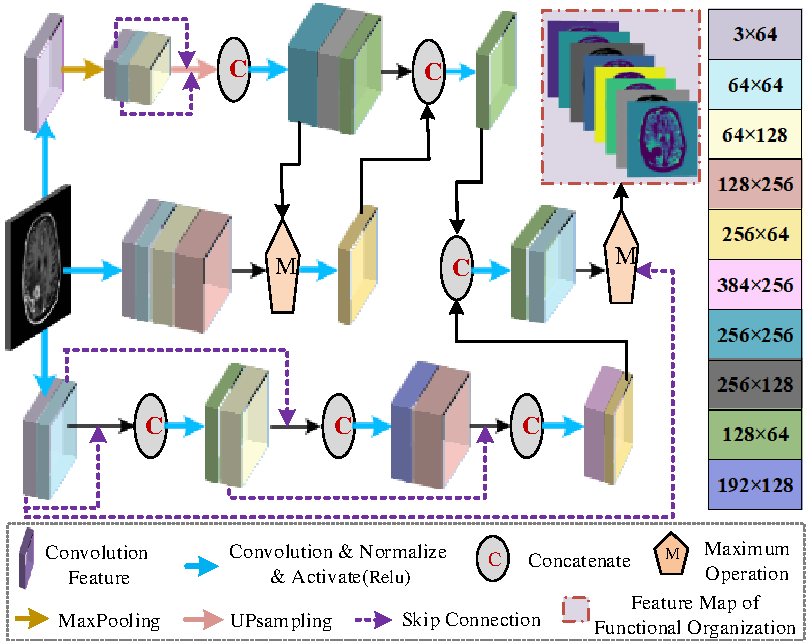
\includegraphics[width=0.9\columnwidth]{figs/paper1cb_work.pdf}
          \caption{GV-Branch提取特征的过程一}\label{paper1cb_work}
     \end{figure}
     
1)通过多尺度策略获得深度卷积特征:由于不同层次和分辨率的卷积运算可以提取不同重要程度的信息,因此提出了一种针对脑影像的功能组织特征提取方法。该方法的功能组织特征分支网络如图\ref{paper1cb_work}所示。网络块主要包括卷积层、池化层、上采样和跳跃连接操作。图\ref{paper1cb_work}给出了获取MS-Info的具体步骤,不同的色块表示不同数量的输入和输出通道,其对应于不同厚度。

多次使用拼接可以扩展高维特征,更准确地发现更重要的语义特征。当多条分支合并时,采用最大值法突出高频纹理信息。由于各种脑部疾病是不均匀的,使用这种特征提取策略可以使病变程度和正常组织之间的分类更加明显。然后,可以更容易地确定PET影像中的局部区域是否异常,并在CT影像中观察到清晰的轮廓和全局结构信息。并且,使用长短跳来增强图\ref{paper1cb_work}中带有紫色虚线的特征的转移,可以充分融合不同层次的视觉特征,减少特征转移过程中的特征损失。这个想法受到DenseNet\cite{2016Densely}的启发,DenseNet主要由许多密集的网络块实现。为了解决消失梯度问题,网络只级联卷积操作的前后层的权重系数,而不级联池化操作。在本节的网络中,将前一层和前一层的特征输入到下一层,连接模态表示为式(\ref{skipfunciton}):

     \begin{equation}\label{skipfunciton}
        f_{d}=H_{d}([f_{0},f_{1},...,f_{d-1}]),
     \end{equation}
     
   \begin{figure}[htb]
      \centering
      % Requires \usepackage{graphicx}
          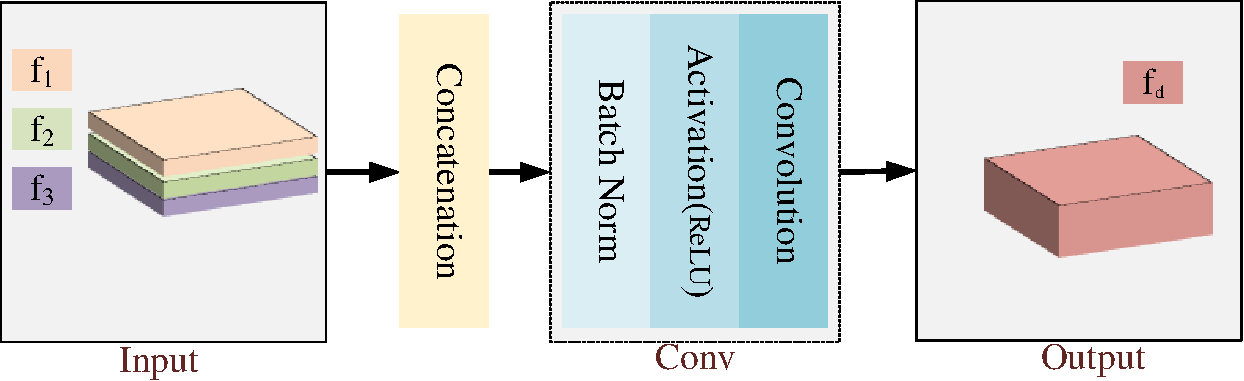
\includegraphics[width=0.9\columnwidth]{figs/paper1skip.pdf}
          \caption{特征跳跃策略}\label{paper1skip}
     \end{figure}
     
其中,$f$表示输出,$d$表示网络中的层数,$H_{d}(*)$表示非线性传递函数的组合,包括级联、BN、激活和卷积操作。多层特征(不一定是相邻层)的并行输入由组合函数操作以获得新特征。新特征的通道数由不同的卷积参数决定。详细步骤如图\ref{paper1skip}所示。此操作有助于捕获跨区域的长期和多层依赖关系,并减少特征转移过程中的损失。因此,可以保留更完整的脑影像结构。


2)通过颜色空间变换获取亮度信息:HSV颜色模型,基于对色彩的直觉理解构建而成,由色调(Hue)、饱和度(Saturation)和亮度(Value)三个参数组成,并以其几何表示而著称于六角锥体模型。HSV颜色空间可以单独处理,并且彼此独立。因此,通过采用HSV颜色模型进行影像分析与处理时能够显著降低复杂度,并且相比RGB色彩空间,HSV更贴合人类视觉系统的自然感知方式。在此特征提取部分,本节计算功能影像的HSV空间的V分量,以提取其亮度特征用于后续处理,如图\ref{paper1FO2_hsV}所示。在该图中,$I_p$表示原始RGBA影像,$I_A$表示RGB影像,$V$表示将$I_p$变换到HSV空间之后的亮度分量。为了进一步增强亮度明显区域的局部信息,本节定义了一个新的亮度值$V'$,如算法\ref{paper1algorithm1}所示。 
   \begin{figure}[htbp]
      \centering
      % Requires \usepackage{graphicx}
          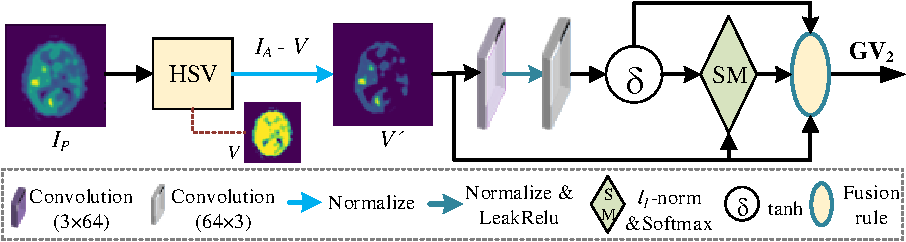
\includegraphics[width=0.9\columnwidth]{figs/paper1FO2_hsV.pdf}
          \caption{GV-Branch提取特征的过程二}\label{paper1FO2_hsV}
     \end{figure}


    \begin{algorithm}[ht]
    \caption{New Luminance Computation}\label{paper1algorithm1}
    \centering
    \begin{algorithmic}[1]
    \Require RGBA image $I_p: (R, G, B, A)$
    \Ensure New luminance value $V'$
    %\STATE
    \State {\textbf{newLum}} $(I_p)$:
    \State \hspace{0.5cm}$I_{A} \gets$ \text{Compress} $(I_p)$;
    \State \hspace{0.5cm}$I_{HSV}: (H, S, V) \gets$ \text{Conver} $(I_p)$;
    \State \hspace{0.5cm}$V' \gets$ $I_{A} - V$;
    \State \hspace{0.5cm}\textbf{return} $V'$;
    %\STATE 
    \State {\textbf{Compress}} $(I_p)$:
    \State \hspace{0.5cm}$I_{A} \gets$ $I_p:(R) + I_p:(G) + I_p:(B)$;
    \State \hspace{0.5cm}\textbf{return} $I_{A}$;
    %\STATE
    \State {\textbf{Conver}} $(I_p)$:
    \State \hspace{0.5cm}$I_{A} \gets$ \text{Compress} $(I_p)$;
    \State \hspace{0.5cm}$I_{HSV} \xleftarrow{Eq.~(\ref{Hcomponent})} I_{A}$;
    \State \hspace{0.5cm}\textbf{return} $I_{HSV}: (H, S, V)$;
    \end{algorithmic}
    \end{algorithm}

如图\ref{paper1FO2_hsV}所示,$I_p$是PET影像的一部分。图中可以发现三个不同的色块(黄色,浅绿色和深蓝色),它们表明能量高或新陈代谢旺盛的区域。病变最有可能存在于这些区域。这些颜色块可以从$I_p$的前景中辨别出来,主要是因为它们的亮度信息。然而,从亮度影像$V$中可以看出,这些有意义的区域还不够清晰,无法准确地定位病变。在算法 \ref{paper1algorithm1}中,本节通过$I_A-V$计算差分影像,以进一步突出这些色块。然后,病变可以清楚地定位在$V'$影像的右侧。基于新的亮度影像,通过后续过程提取HSV颜色空间中的深度特征$GV_2$,如图\ref{paper1FO2_hsV}所示。
  
  
\subsubsection{双分支的分层融合与重构}
为了充分利用从两个分支中提取的深层MS-Info特征,本节采用了基于分类和分层的融合策略,如图\ref{paper1Framework}的融合规则阶段所示。在第一层融合解剖结构特征(SF和GV$_1$),然后在第二层融合功能代谢特征(GV$_2$),有利于保留和增强待融合医学影像的关键MS-Info。本节的融合策略不是一个简单的加权和。为了保持和增强多模态影像的重要纹理特征,使用最大化操作。同时,使用卷积和激活函数来获得局部细节结构特征。如图\ref{paper1Framework}所示,采用$tanh$作为激活函数。 


\subsubsection{损失函数构建及参数设置}
由于医学数据的保密性,大量的多模态医学数据不易获取。通常,许多基于ImageNet数据训练的网络模型,如ResNet\cite{2016Inception}和VGG\cite{2015Places205},被选择来生成预训练参数。为了在解决梯度破碎问题和收敛速度方面获得更好的性能,本节选择ResNet101来迁移ImageNet上的最后一个卷积特征,也就是说,使用在ImageNet数据上预训练的ResNet101的最后一层作为本节的第一个卷积层来提取有效的影像特征。由于预训练模型是针对分类任务设计的,因此在本节的网络结构中,第一层的参数会根据本节的任务进行调整,以达到更好的融合效果。为了获得源影像的更精确的重建,本节联合结构和像素信息来构造损失函数如下式(\ref{paper1loss_function}):
     \begin{equation}\label{paper1loss_function}
       L=\omega L_{S} + (1-\omega)L_{P}
      \end{equation}

总损失函数由结构相似度$L_{S}$和像素损失$L_{P}$组成,$\omega$为调整系数,其值由训练和测试效果根据不同取值而定。$I_f$表示融合的结果,$I_i,i=1,2$表示输入的源影像。SSIM表示两个影像的结构相似性[44]。对于这两种类型的影像,计算结构相似度并将其组合。假设两个影像的结构相似度为$F_{SSIM_i}$,$F_{SSIM_i}= 1-SSIM(I_f,I_i),i=1,2$,总结构相似度函数计算如下:

     \begin{equation}\label{paper1L_{SSIM}}
        L_{S}=\sum_{i=1}^2\alpha_i\left(1-\frac{\left(2 \mu_{I_f} \mu_{I_{i}}+c_{1}\right)\left(2 \sigma_{I_f}\sigma_{ I_{i}}+c_{2}\right)}{\left(\mu_{I_f}^{2}+\mu_{I_{i}}^{2}+c_{1}\right)\left(\sigma_{I_f}^{2}+\sigma_{I_{i}}^{2}+c_{2}\right)}\right)
      \end{equation}
其中,$\mu_{I_f}$是$I_f$的平均值,$\mu_{I_{1}}$和$\mu_{I_{2}}$分别是$I_{1}$和$I_{2}$的平均值。$\mu_{I_f}^{2}$是$I_f$的方差,$\mu_{I_{1}}^{2}$和$\mu_{I_{2}}^{2}$分别是$I_{1}$和$I_{2}$的方差。$\sigma_{I_f I_{1}}$和$\sigma_{I_f I_{2}}$是原始影像和融合影像之间的协方差,$c_{i}$是常数。像素损失是$l_{2}$范数。假设两幅影像的像素损失为$F_{M_i}$,$F_{M_i}= \left\|I_f-I_i \right\|_2$,则总像素损失函数计算如下:

      \begin{equation}\label{paper1L_{P}}
       L_{P}= \beta \sum_{j=1}^{n}\left(I_{f_{j}}-I_{1_{j}}\right)^{2}+
       (1- \beta)\sum_{j=1}^{n}\left(I_{f_{j}}-I_{2_{j}}\right)^{2}
      \end{equation}
在式(\ref{paper1L_{SSIM}})和式(\ref{paper1L_{P}})中,$\alpha_i,i=1,2$,$\beta $是设置在区间$[0,1]$中的权重参数。在本节中,这三个参数都设置为0.5。在方程式(\ref{paper1loss_function})中,$\omega\in[0,1]$的取值由训练效果和测试效果决定。参数$\omega$决定了不同模态原始影像与融合结果影像之间相关性的程度。在其他参数不变的情况下,通过观察不同$\omega$的融合影像的效果来确定它的取值,如图\ref{difOmega}所示。
   \begin{figure}[htbp]
      \centering
      % Requires \usepackage{graphicx}
          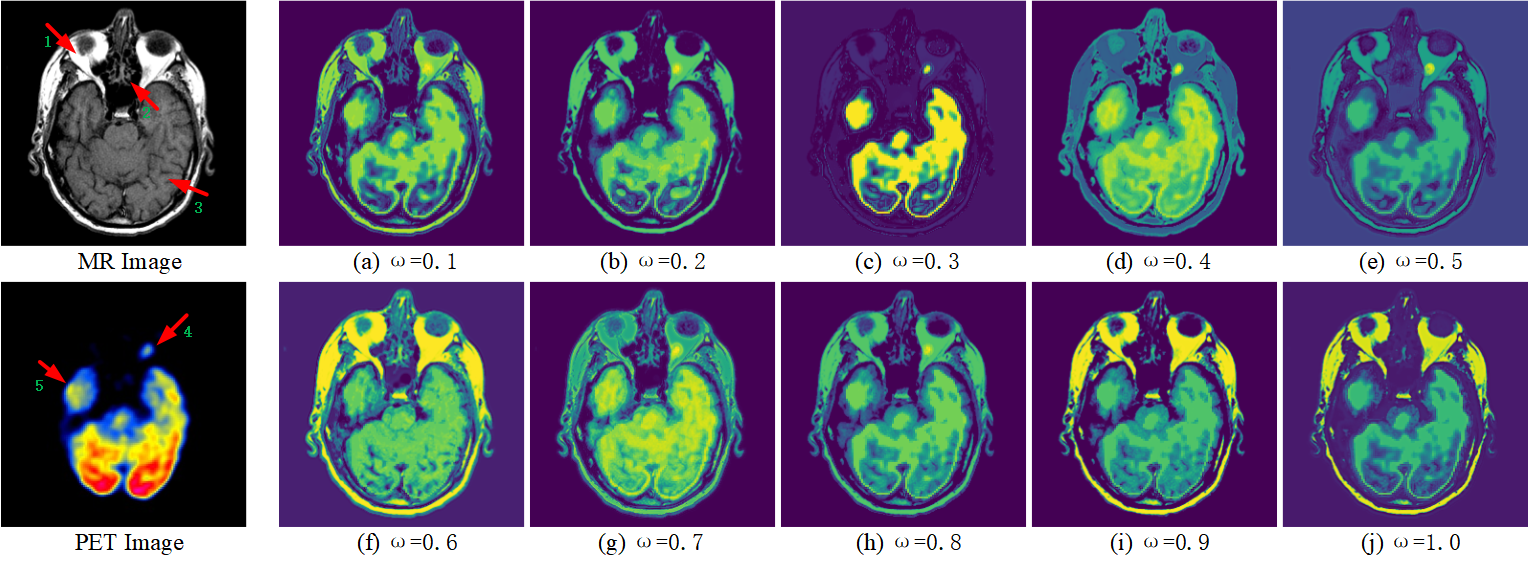
\includegraphics[width=0.9\columnwidth]{figs/difOmega.png}
          \caption{不同的$\omega$值应用于MRI-PET影像融合的结果 }\label{difOmega}
     \end{figure}
     
\begin{table*}[ht]
\centering
\caption{针对不同$\omega$取值下的MRI-PET影像融合的质量评估}\label{difOmega_evaluation}
\begin{tabular}{m{2cm}<{\centering}m{3cm}<{\centering}m{3cm}<{\centering}m{3cm}<{\centering}} 
\hline
\textbf{$\omega$} & \textbf{EN}     & \textbf{SD}      & \textbf{VIF}   \\\hline
0.1        & 3.3390          & 46.1341          & 0.2065          \\
0.2        & 3.1554          & 44.4309          & 0.2087          \\
0.3        & 3.2173          & 47.9444          & 0.0395          \\
0.4        & 3.7952          & \textbf{51.3496} & 0.2017          \\
0.5        & 4.0602          & 26.4541          & 0.0443          \\
0.6        & \textbf{4.5183} & 46.2509          & 0.2243          \\
0.7        & \textbf{4.3093} & \textbf{51.8038} & \textbf{0.2801} \\
0.8        & 3.1933          & 45.3808          & 0.2378          \\
0.9        & 3.1667          & 47.9978          & \textbf{0.2871} \\
1.0        & 3.9747          & 35.0954          & 0.1738      \\ \hline   
\end{tabular}
\end{table*}
本节通过实验来解释$\omega$的影响,并为$\omega$设置了一组值{0.1,0.2,0.3,0.4,0.5,0.6,0.7,0.8,0.9,1.0}。在图\ref{difOmega}中,第一列显示了MRI和PET影像,其他影像是采用不同$\omega$的融合结果。从图中可以直观地观察到,当$\omega$小于0.5时,融合结果中的MRI信息损失更大,尤其是当0.3最严重。当$\omega$大于0.5时,融合结果中PET的亮度信息或多或少会丢失或失真。只有当$\omega$为0.7时,PET的亮度信息才能得到最好的保留,MRI的边缘轮廓信息也很清晰。
表\ref{difOmega_evaluation}显示了图\ref{difOmega}中不同$\omega$下MRI-PET融合的三个指标。EN表示信息熵,SD表示标准差,VIF是对人类视觉感知的评估。这三个值越大,融合影像质量越好。融合影像质量评估指标的计算结果与上述观察结果一致。当$\omega$为0.7时,三个指标值达到最佳平衡和优化状态,其中SD最好,EN和VIF接近最佳值。


综上所述,当$\omega$取0.7时,得到的结果最好。因此,本节在实验中选择该值来测试融合效果。在训练过程中,初始学习率为0.001,250 epoch,批量大小为2,采用批量归一化,优化函数为Adam。此外,本节实施了一种自适应损失调整方案,即每隔50个训练周期将学习率调整为初始值的10\%,因为在训练过程中使用较小的学习率来调整权重以获得更好的权重。本节的方法已经在PyTorch版本1.5.0及其相应的CUDA版本10.1下的Python 3.7.9中实现。

\subsection{多模态脑影像融合的实验}
为了进一步验证所提出融合技术的效能,实验在不同的大脑影像对(MRI-SPECT/MRI-CT/MRI-PET)上进行。从ADNI(http://adni.loni.usc.edu/data-samples/access-data/)中获得了总共555个MRI-PET影像对作为训练集,其大小为256×256。在测试MRI-CT、MRI-SPECT和MRI-PET影像对中使用了全脑图谱 (http://www.med.harvard.edu/aanlib/)上的30对影像,包括脑血管疾病(中风)和肿瘤疾病(脑肿瘤)。所有实验都在GeForce RTX 3090 Ti 12 Intel Core Interl(R)Xeon(R)CPU E5-2678 v3 2.50 GHz 64 GB RAM设备的GNU/Linux x86 64系统上进行。

对于每对影像的实验,本节使用所提出的MsgFusion和其他九种代表性的方法(LatLrr\cite{2018Infrared},IFCNN\cite{2020IFCNN},NestFuse\cite{2020NestFuse},atsIF\cite{2020An},FusionDN\cite{2020FusionDN},FusionGAN\cite{2019FusionGAN},FunFuseAn\cite{kumar2019structural},WPADCPCNN\cite{panigrahy2020mri}和OLTPSpS\cite{das2022optimized})得到融合结果。并采用EN\cite{roberts2008assessment}、SD\cite{shi2005wavelet}
、MI\cite{qu2002information}、rSFe\cite{2007A}、SM\cite{Piella2003IP}、VIF\cite{han2013new}等6种常用的评价指标和一种相对新颖的指标$R_{Q}^{(F/(AB))}$(简称RQ)\cite{sengupta2020edge}来评价这10种方法的融合效果。RQ通过计算分数阶微分来反映融合影像中保留了多少边缘信息,它取代了\cite{Xydeas2000Objective}中使用的噪声敏感的Sobel算子,文章中采用三个Sigmoid函数(tanh、arctan、Logistic)来得到三个度量。考虑到它们共同的函数单调性,本节只选择了一个基于Logistic函数的度量应用于本节的实验中。由于不同指标的值相差很大,本节进行了适当的线性变换,图\ref{paper1MPDindex}和图\ref{paper1CMDindex}的左上角标出了这些变换,以方便在同一图中进行比较。

\subsubsection{MRI-SPECT影像对的融合}
图\ref{paper1mpd008roi}中的第一列显示源MRI和SPECT影像。MRI清晰显示脑脊液和其他软组织的纹理细节。SPECT上的不同颜色和亮度可以反映代谢信息。图\ref{paper1mpd008roi}(a)-(i)示出了所考虑的十种融合方法的结果。图\ref{paper1mpd008roi}(j)展示出了通过MsgFusion获得的融合结果。聚焦于由七个箭头指示的区域,可以看出,与由其他七种方法获得的融合影像中的对应区域相比,显示出更清晰的结构和纹理细节。结合临床信息,本节分析了MRI和SPECT的MS-Info是否很好地保留在图\ref{paper1mpd008roi}(j)中蓝色矩形框内箭头指示的7个区域的融合结果中。

     \begin{figure*}[ht]
      \centering
       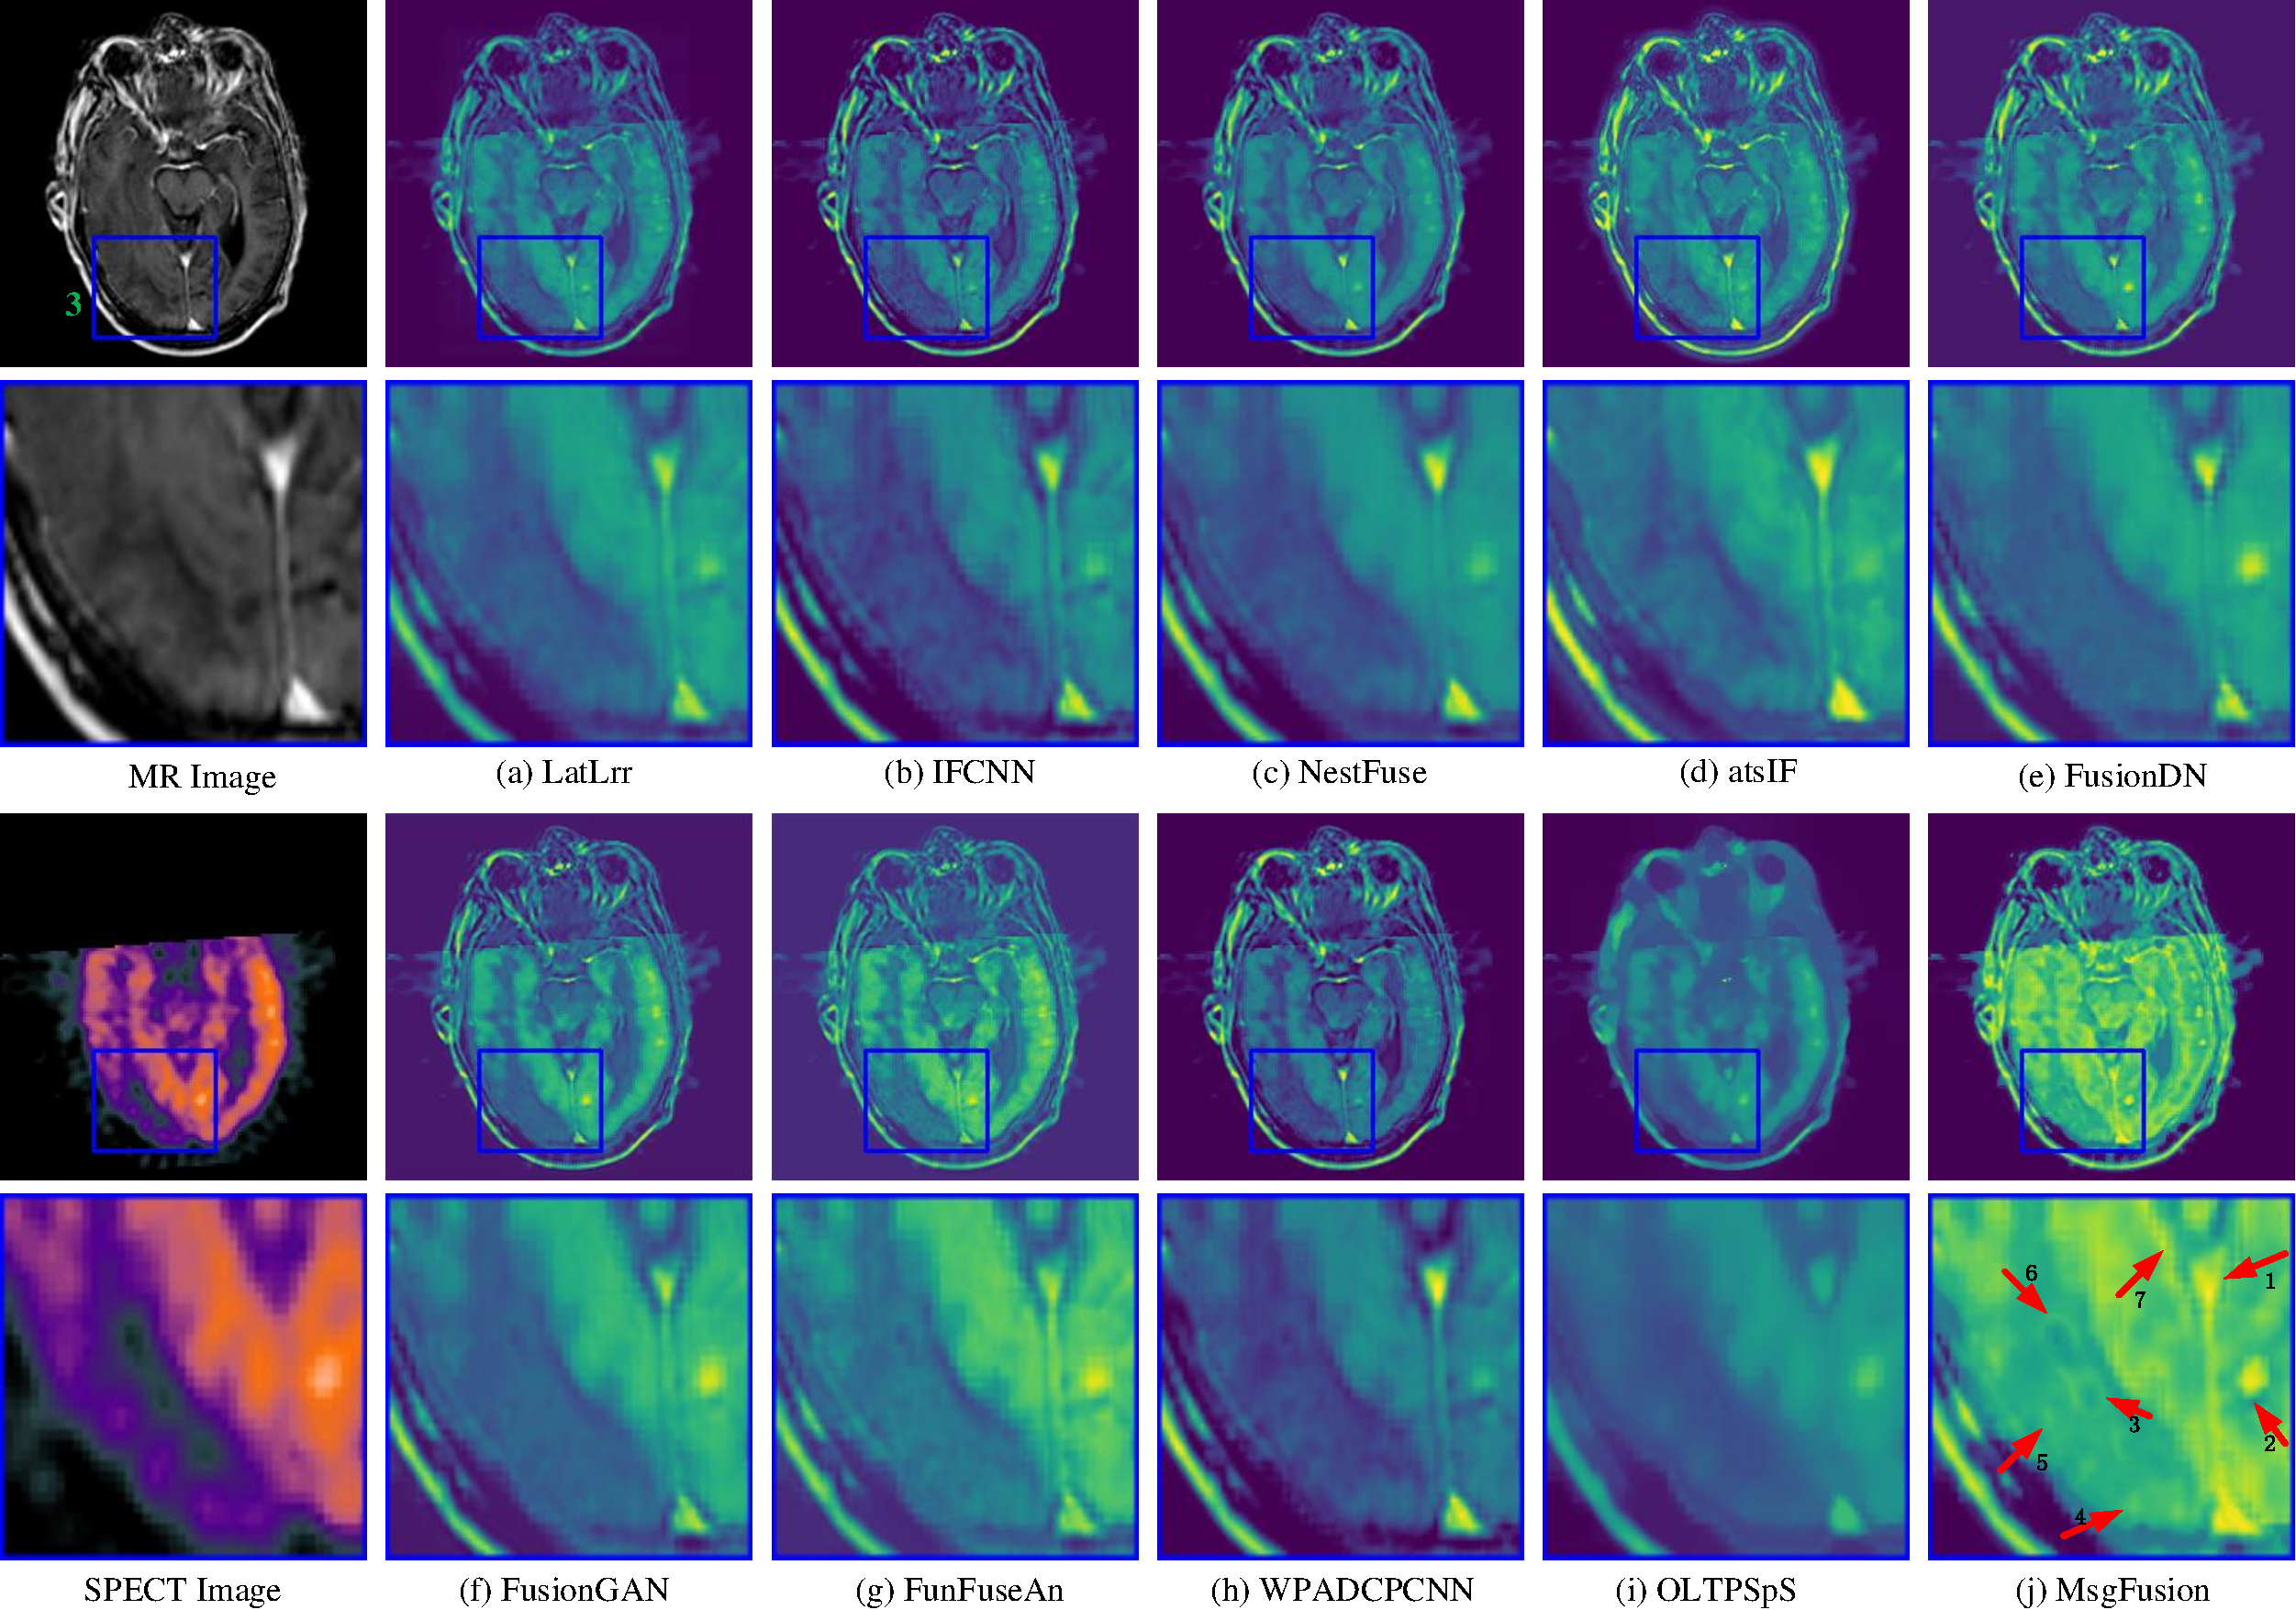
\includegraphics[width=0.9\textwidth]{figs/paper1mpd008roi.pdf}
      \caption{用于脑MRI-SPECT影像融合的不同方法(LatLrr、IFCNN、NestFuse、atsIF、FusionDN、FusionGAN、FunFuseAn、WPADCPCNN、OLTPSpS和本节提出的MsgFusion)性能比较} \label{paper1mpd008roi}
     \end{figure*}
     
箭头1指向小脑结节区域,MRI源影像上可见一个轮廓清晰的白色小三角形,右上角略有模糊。然而,在SPECT源影像中,没有明显的特征。在LatLrr的融合结果中,影像显得模糊,与周围组织无法区分。在IFCNN、NestFuse和FusionDN的融合结果中,它们都比SPECT保留了更多的MRI信息。右上角的增强效果不明显。FusionGan和FunFuseAn结果中的小三角形扭曲。在OLTPSPS的融合结果中,亮度信息明显丢失。

箭头2为左小脑半球区域,主要来自SPECT影像,表现为边缘模糊的亮点,在MRI上看起来像一个小黑洞。在LatLrr、IFCNN、NestFuse、atsIF、WPADCPCNN和OLTPSpS的融合结果中,不容易找到那个亮点。在FusionGAN和FunFuseAn的融合结果中,亮点增强,但略有模糊。在FusionDN的融合结果中,这一亮点很明显,但与周边机构融合,具体位置无法确定。MsgFusion的融合结果中,有明显的亮度和轮廓,位置准确。

箭头3和6代表右小脑半球区域。在MRI中,它是具有灰度值,形状像一片树叶。在SPECT影像中,有三个相邻的灰色空环。从SPECT影像中可以发现,在箭头6指示的位置有一个清晰的灰色空环。在NestFuse和atsIF获得不均匀分布区域的融合影像中可以识别它,但不是很清晰,箭头3处的环消失不见。在IFCNN、FusionDN、FusionGAN、FunFuseAn和WPADCPCNN的融合结果中,它们在第6个ROI的环更清晰,而在第3ROI则不清晰。在本节提出的方法中,几个环可以很好地显示出来,并且很容易找到它们的位置。

箭头4和5分别是枕骨和右小脑半球的边缘区域。MRI中的这个区域看起来像花边,但不容易检测到。它在SPECT中表现为一个不明显的亮度小点。相比之下,MsgFusion保留了MRI的边缘,并且可以很容易地在SPECT中找到几个点。区域7是小脑结节附近的右鞍半球边缘。在由浅白色边缘信息表示的MRI中,在SPECT影像中似乎存在一条直线。对于所有方法的不同结果中,只有MsgFusion可以清楚地找到其边缘。

    \begin{figure}[ht]
      \centering
      % Requires \usepackage{graphicx}
          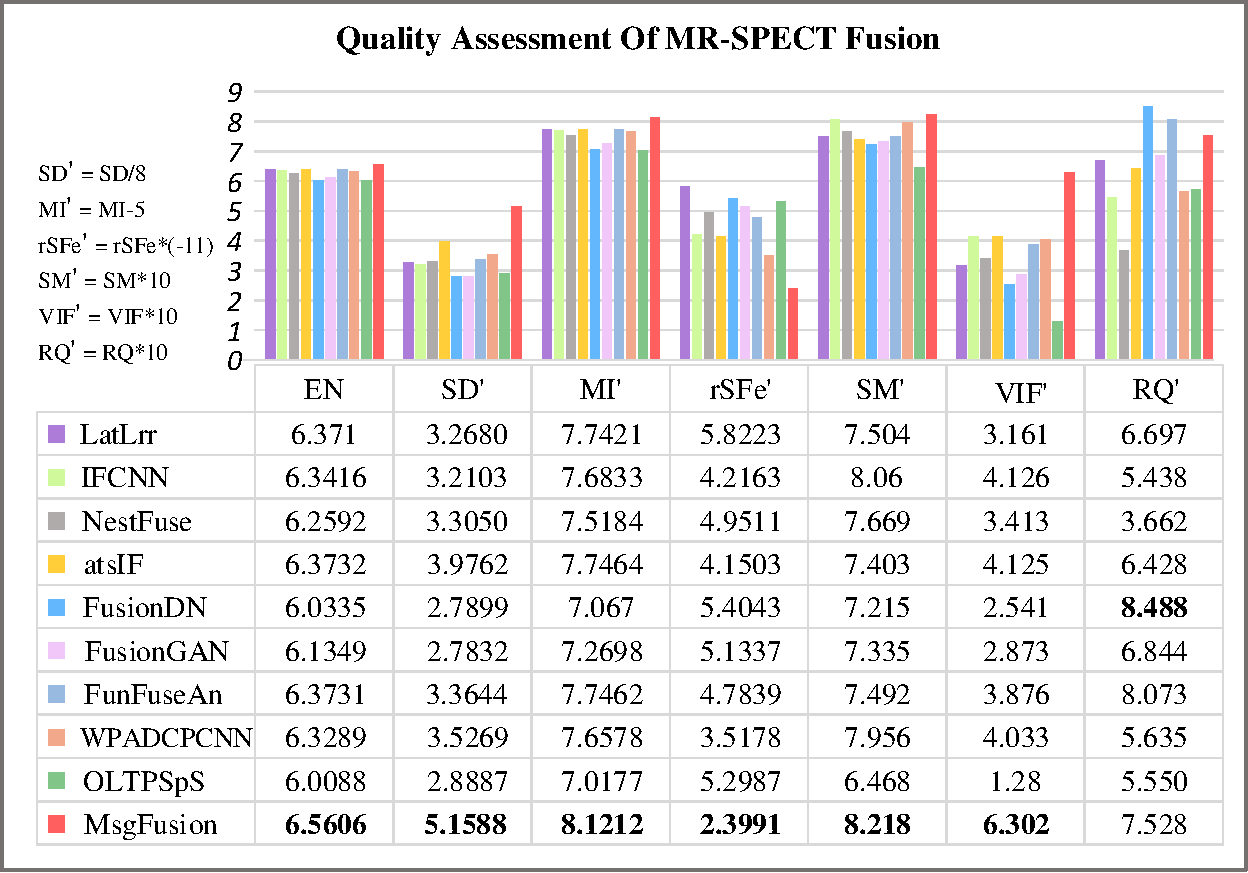
\includegraphics[width=0.9\columnwidth]{figs/paper1MPDindex.pdf}
          \caption{计算不同方法对MRI-SPECT融合的质量评估指标值}\label{paper1MPDindex}
     \end{figure}

图\ref{paper1MPDindex}显示了图\ref{paper1mpd008roi}中融合结果的评估指标,不同的颜色柱条对应不同融合方法。EN、SD、MI、SM、VIF、RQ分别表示融合的熵、标准差、互信息、结构相似度、视觉信息保真度和边缘信息,这些值越大,融合效果越好。rSFe反映了改善的空间频率,其绝对值越小,融合效果越好。除RQ外,其他6个评价指标均表明MsgFusion方法达到最佳融合效果。因此,本节的融合结果具有更合适的亮度、更清晰的轮廓和更精细的纹理。此外,本节的结果保持并增强了重要的医学信息。当大脑出现异常时,可以通过观察SPECT的颜色和亮度信息,并结合MRI的纹理进行有效的分析,来确定可能的疾病类型。

\subsubsection{MRI-CT影像对的融合}
图\ref{paper1cmd010roi}中的第一列显示了原始CT和MRI。很容易在CT影像上找到硬轮廓,如骨骼,在MRI上找到软组织结构。右边是不同融合方法的结果。图\ref{paper1cmd010roi}(j)展示出了MsgFusion的融合结果和获得的局部放大影像,主要关注由箭头指向的六个ROI。

    \begin{figure*}[ht]
      \centering
      % Requires \usepackage{graphicx}
          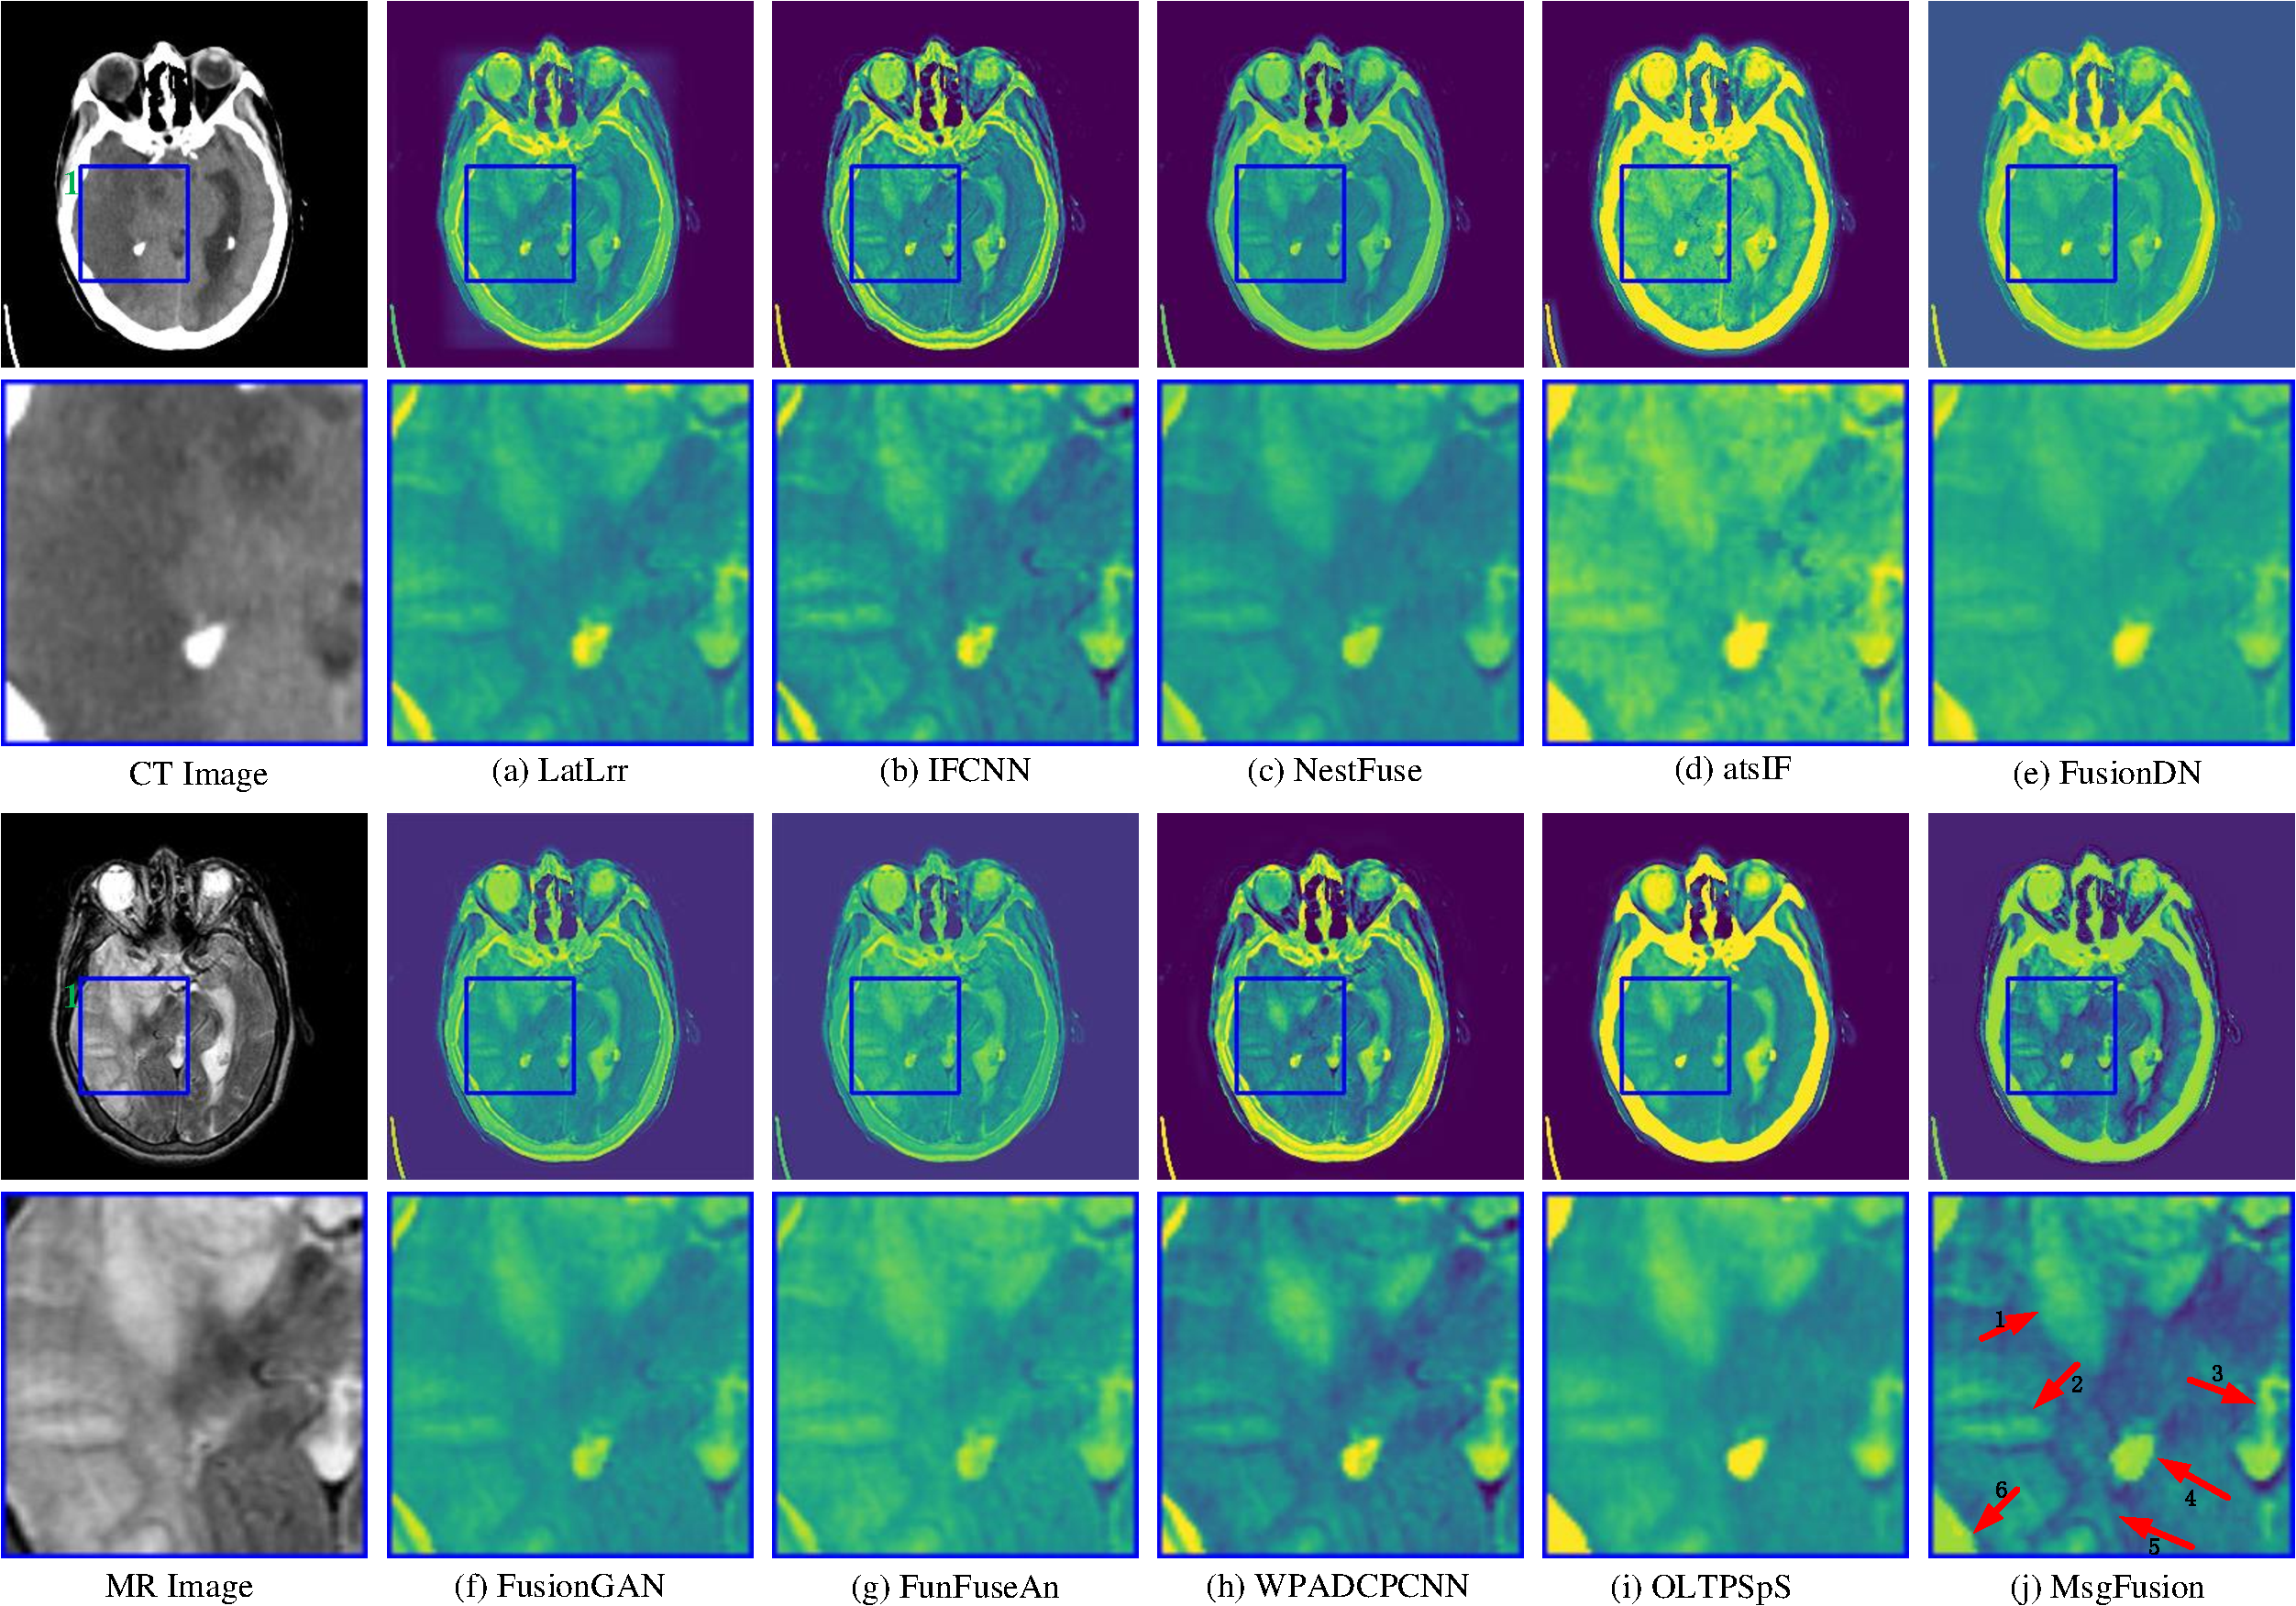
\includegraphics[width=0.9\textwidth]{figs/paper1cmd010roi.pdf}
          \caption{用于脑MRI-CT影像融合的不同方法(LatLrr、IFCNN、NestFuse、atsIF、FusionDN、FusionGAN、FunFuseAn、WPADCPCNN、OLTPSpS和本小节提出的MsgFusion)性能比较}\label{paper1cmd010roi}
     \end{figure*}

箭头1指向的区域代表侧脑室的下角,在CT影像上为深灰色,在MRI上为明亮而清晰。MRI中ROI 1的面积较大,具有重要的MS-Info信息,常被用来判断是否存在病变。在LatLrr、IFCNN、FusionDN、FunFuseAn和OLTPSps的融合结果中,轮廓不明显且不容易找到。在atsIF结果中,位置的亮度得到改善,但边缘出现了平滑现象。在FusionGAN和WPADCPCNN的融合结果中,位置的边缘分类明显,但亮度不够。在本文的融合结果中,可以很容易地找到区域及其边界。箭头2指向的区域呈岛状,主要反映在MRI上。这一区域并不像正常脑部影像中显示的那样完整,这表明组织失去了水分或萎缩。在图\ref{paper1cmd010roi}中可以发现,只有MsgFusion融合结果中的区域明显,并显示出有别于其他组织的清晰轮廓。箭头3指向的区域在CT影像上为第四脑室,在MRI上也有脑桥和基底动脉的部分信息相连。atsIF方法的亮度具有良好的亮暗影像对比度,然而,该区域的结构完整性被破坏。ROI 3中的其他算法的结果清晰但不够明亮,而WPADCPCNN和MsgFusion更好。

箭头4指向的区域为侧脑室后角,主要表现在CT影像上。它在MRI上不是特别明显,但是,通过与周围组织仔细区分可以发现。对于LatLrr、IFCNN、Nesthood和FusionGAN,可以找到ROI 4的轮廓,但其边界附近存在伪影,亮度信息不足。对于FusionDN,这个位置很明显,但周围组织丢失。FunFuseAn融合结果表明,融合区域变得模糊。OLTPSpS的结果有足够的亮度,但面积略小。在本节提出的方法中,ROI 4不仅具有清晰的轮廓和明显的边界,而且具有足够的亮度。在本节提出的方法中,侧脑室后角的重要医学特征存在并得到增强。

箭头5指向的区域为中央沟,主要表现在MRI上。该位置的密度和亮度信息可以帮助医生确定是否存在异常。对于MsgFusion区域,它具有清晰的轮廓和亮度信息,很容易找到。箭头6指向的区域为顶骨,主要在CT影像上反映。当这个区域有边缘缺损或不完整时,就可以判断是否有脑损伤。通过以上分析,可以表明MsgFusion具有相对更好的融合效果。

  \begin{figure}[ht]
      \centering
      % Requires \usepackage{graphicx}
          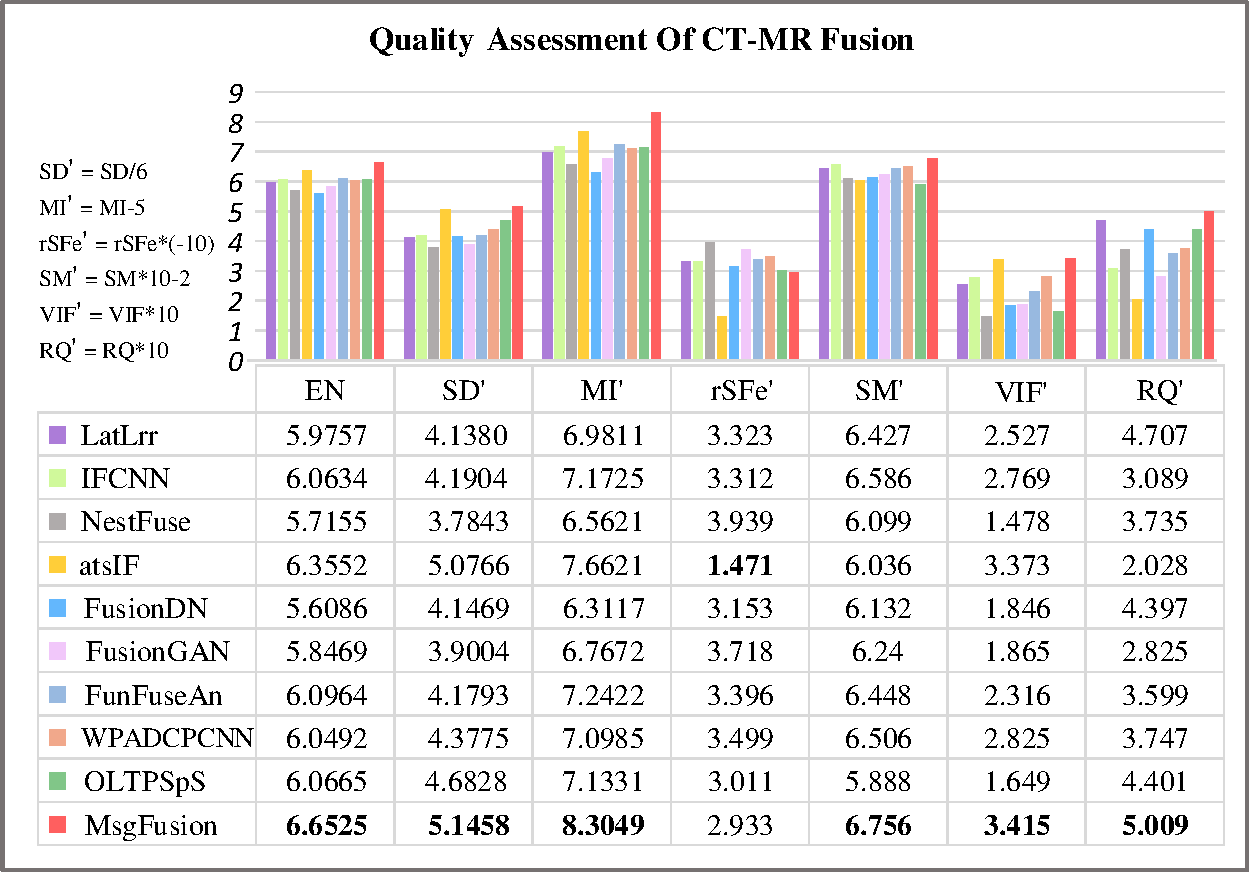
\includegraphics[width=0.9\columnwidth]{figs/paper1CMDindex.pdf}
          \caption{计算不同方法对MRI-CT融合的质量评估指标值}\label{paper1CMDindex}
     \end{figure}
     
此外,图\ref{paper1CMDindex}展示出了对应于图\ref{paper1cmd010roi}的质量评估指标值。结果表明,本节的MsgFusion方法在6个指标值上占优势,在rSFe上是次优的。这意味着原始CT和MRI的信息不仅保持良好,而且在本节的方法的融合结果中也得到了增强。当通过观察MRI密度和面积可以确定脑出血时,CT影像可以发现脑出血的大致范围。


%\subsubsection{计算成本}
%在我们的计算环境下,用10种方法对30对不同的数据形态进行了测试。记录每个方法的平均运行时间。所有结果都列在表\ref{paper1timeCost}中。我们可以看到,我们方法的平均运行时间是2.0048秒。虽然这不是一种快速的方法,但时间成本是可以接受的。

\if 0
  \begin{table}[ht]
    \centering
    \caption{影像融合方法的运行时间(单位:s)}\label{paper1timeCost}
    %\footnotesize
    \begin{tabular}{ccccc}
    \toprule[1pt]
     LatLrr &IFCNN &NestFuse &atsIF &FusionDN \\ \hline
     %1238.7976  &6.7223 &29.2867   &203.9445   &20.6184 \\ \hline
     41.2933  &0.2241 &0.9762   &6.7982   &0.6873 \\ \hline
     FusionGAN  &FunFuseAn &WPADCPCNN &OLTPSpS &MsgFusion\\ \hline
     %14.7726  &10.7955 &1190.1147 &1457.83 &60.1435\\
     0.4924  &0.3599 &39.6705 &48.59 &2.0048\\
    \bottoMRIule [1pt]
    \end{tabular}
 \end{table}
\fi

\subsubsection{影像融合的问卷调查}
对于医学影像融合,最终的目标是为医生提供易于观察的融合影像,以便对病变进行定性、定量和定位分析。因此,这种主观评价可以证实MsgFusion方法在临床意义上的优势。为了验证算法的临床有效性,本节对融合效果进行了在线问卷调查,并分发给了不同医院神经内科和医学影像科的30名医生。这些医生的临床经验:10年以上15人,5-10年3人,3-5年6人,3年以下6人。在这份问卷中,本节根据15组融合实验设计了15个问题。对于每个问题,将6种有代表性的方法(即LatLrr、NestFuse、atsIF、FusionGAN、FunFuseAn和MsgFusion)的融合影像作为选项。不同方法得到的融合影像的顺序是随机排列的。每个受访者被允许选择一个或两个具有最佳融合结果的选项作为每个问题的答案。医生不需要确定融合后的影像保留了多少原始影像信息。他们只需要根据他们的临床经验来判断哪些融合结果更有利于他们的观察和临床诊断。最终,收到了29名参与者的有效答案。
\begin{table}[htbp]
    \centering
  \caption{统计问卷调查表中临床医生选择各种方法的融合影像次数}\label{paper1Questionnaire}
  \small
\begin{tabular}{ccccccccccccccccc}
\hline
& \textbf{LatLrr} &\textbf{NestFuse} &\textbf{atsIF} &\textbf{FusionGAN} &\textbf{FunFuseAn} &\textbf{MsgFusion}
\\ \hline
 \textbf{$Q_1$} & 6 & \textcolor{red}{16} & \textcolor{blue}{9} & 7 & 0 & 7 \\ 
 \textbf{$Q_2$} & \textcolor{red}{12} &\textcolor{blue}{10} & 7 & 8 & 1 & 5 \\ 
 \textbf{$Q_3$} & \textcolor{blue}{9} & 7 & 7 & 7 & 1 & \textcolor{red}{12} \\ 
 \textbf{$Q_4$} & 5 & \textcolor{blue}{9}  & 5 & 0 & 6 & \textcolor{red}{17} \\ 
 \textbf{$Q_5$} & 3 & 8 & \textcolor{blue}{10} & 6 & 4 & \textcolor{red}{12} \\ 
 \textbf{$Q_6$} & 3 & \textcolor{blue}{10} & 2 & 4 & 4 &{\textcolor{red}{21}} \\ 
 \textbf{$Q_7$} & 7 & 8 & \textcolor{blue}{9} & 2 & 5 & \textcolor{red}{13} \\ 
 \textbf{$Q_8$} & 4 & 6 & 8 & \textcolor{blue}{10} & 4 & \textcolor{red}{12} \\ 
 \textbf{$Q_9$} &8 &7 &\textcolor{red}{12} & 4 &\textcolor{blue}{9} &4 \\ 
 \textbf{$Q_{10}$} &4 &1 &5 &\textcolor{red}{15} &7 &\textcolor{blue}{11} \\ 
 \textbf{$Q_{11}$} &7 &6 &\textcolor{blue}{9} &3 &4 &\textcolor{red}{14} \\ 
 \textbf{$Q_{12}$} &4 &5 &\textcolor{red}{15} &2 &6 &\textcolor{blue}{10} \\ 
 \textbf{$Q_{13}$} &10 &5 &3 &\textcolor{red}{11} &6 &\textcolor{blue}{9} \\ 
 \textbf{$Q_{14}$} &6 &6 &\textcolor{blue}{10}&7 &1 &\textcolor{red}{13} \\ 
 \textbf{$Q_{15}$} &\textcolor{blue}{10} &2 &4 &2 &\textcolor{red}{12} &\textcolor{blue}{11} \\ 
 \textbf{$\sum$} &98 &106 &\textcolor{blue}{115}  &88 &70 &\textcolor{red}{172}
               
\\ \hline
\end{tabular}
\end{table}

统计结果如表\ref{paper1Questionnaire}所示,其中记录了从每种方法中为融合影像选择的次数。在用$Q_i(i=1,\cdot\cdot\cdot,15)$标记的每一列中,以下数字对应于医生为六种方法的融合影像选择的次数。在15组实验中,MsgFusion产生的融合影像在8组中被最频繁地选为最佳融合影像,在4组中被第二频繁地选为最佳融合影像。从临床医生的角度来看,MsgFusion的融合效果远远超过其他任何考虑的方法。标记有$\sum$的最后一列列出了其融合影像被选择的每种融合方法的总次数。计算结果表明,本文方法比次优方法选择的次数分别高26.5\%和10.17\%。

   \begin{figure*}[htbp]
      \centering
          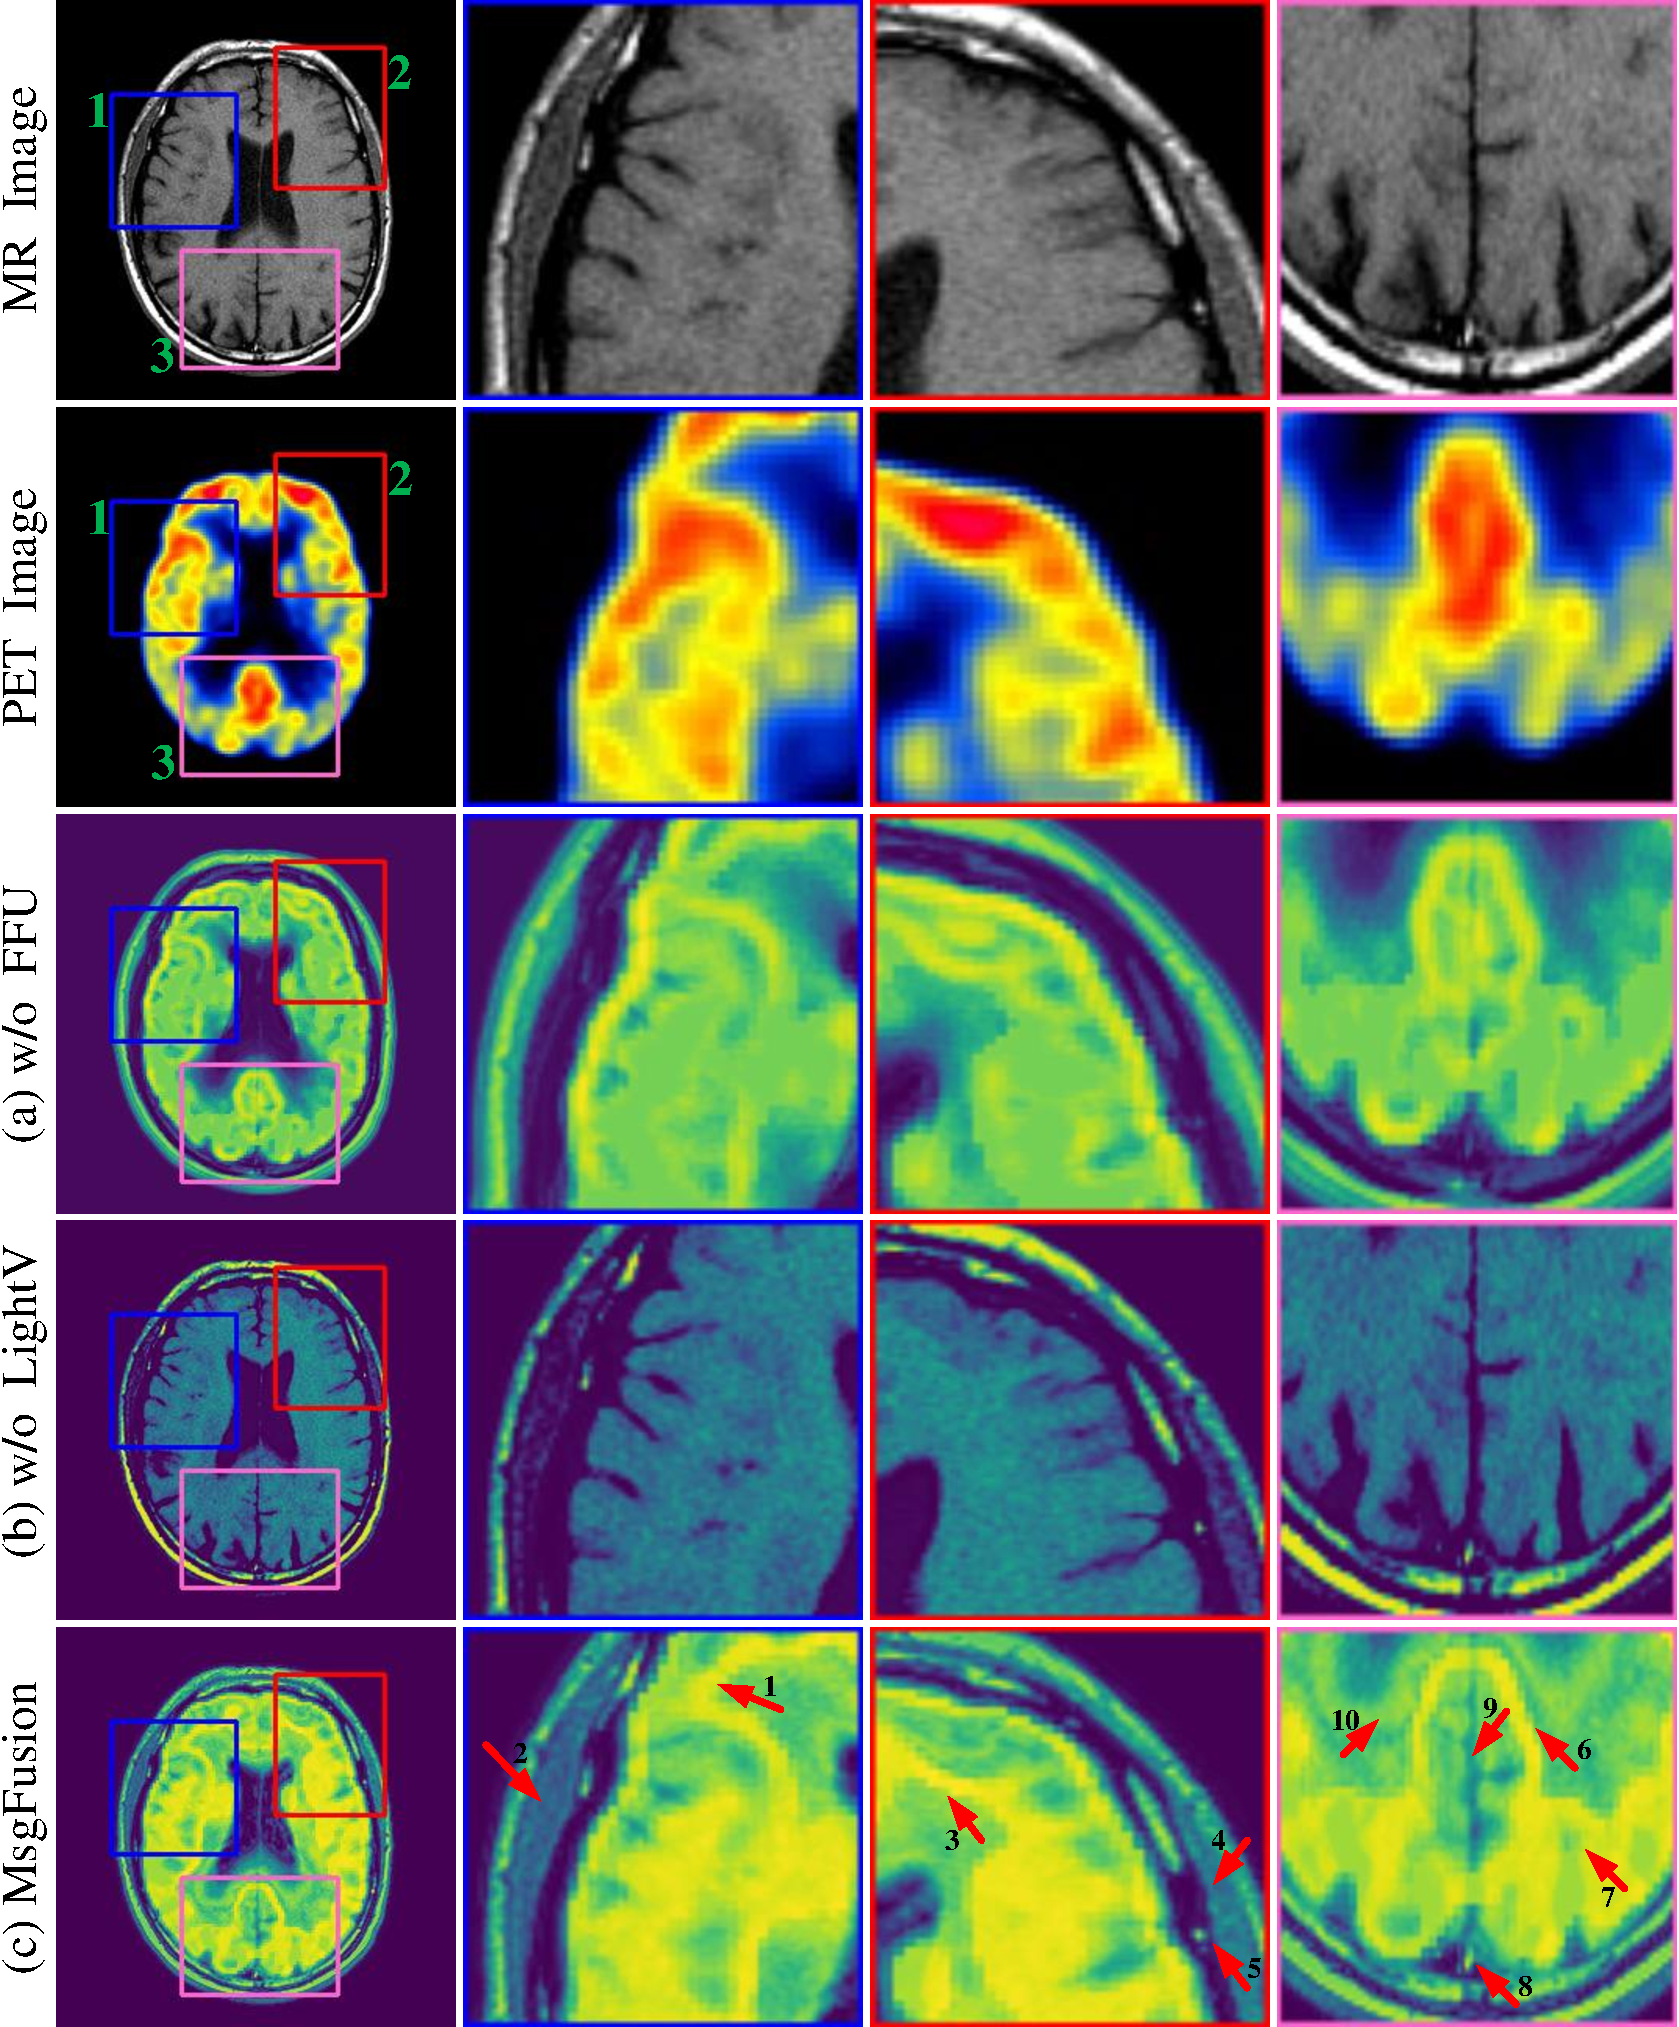
\includegraphics[width=0.8\columnwidth]{figs/paper1noHSVnoFourier_MAD015.pdf}
          \caption{本节所提出的影像融合方法的消融实验}\label{paper1noHSVnoFourier}
     \end{figure*}
     
\subsubsection{影像融合的消融实验}
为了说明在SF-Branch中结合频域和在GV-Branch中结合HSV颜色空间的必要性和有效性,本节对MRI-PET融合进行了消融实验。实验结果如图\ref{paper1noHSVnoFourier}所示。前两行显示MRI和PET的源影像及其各自的三个局部放大的ROI。下面的三行分别显示的是:(a)缺少频域处理,(b)缺少来自HSV颜色空间的改进亮度分量,(c)本节提出的MsgFusion方法。在最后一行局部放大影像中,标记了十个箭头,指向具有明显医学特征信息的区域。箭头1和3指向额叶,箭头2指向的是额骨,箭头4指向的是额骨内面,箭头5指向的是额骨和额叶之间的空间,顶叶区域由箭头6、7和10指示,箭头8指向的是上级矢状窦,并且箭头9指向大脑纵隔。当融合过程中不涉及FFT时,融合结果可以更完整地保留PET中的结构特征,但会丢失更多的MRI信息。当只使用FFT而不考虑HSV颜色空间的改进$V'$分量时,融合结果能较好地保留MRI的完整特征,但不能反映PET的功能信息。如图\ref{paper1noHSVnoFourier}的第五行所示,当同时考虑两者时,融合结果明显变得更好。

     
\begin{table*}[ht]
    \centering
  \caption{图\ref{paper1noHSVnoFourier}中对应的三种融合策略的质量评估}\label{paper1AblationIndex}
\begin{tabular}{ccccccc}
\hline
\textbf{Whole image}  &  EN         &  SD         &  MI         &  rSFe   &  SM         &  VIF  \\ \hline
w/o FFU                   &  \textcolor{red}{ 4.5027}      &  \textcolor{blue}{ 56.8141}     &  \textcolor{red}{ 9.0054}      & -0.5018                        & 0.2704                             &  \textcolor{blue}{ 0.3219} \\ 
w/o LightV                & 3.5768                             & 36.7745                            & 7.1537                             &  \textcolor{red}{ -0.2977} &  \textcolor{red}{ 0.3523}      & 0.1262                        \\ 
MsgFusion             &  \textcolor{blue}{ 4.476}       &  \textcolor{red}{ 67.5634}     &  \textcolor{blue}{ 8.952}       &  \textcolor{blue}{ -0.4103} &  \textcolor{blue}{ 0.3205}      &  \textcolor{red}{ 0.4076} \\ \hline
\textbf{Average ROIs} &  EN         &  SD         &  MI         &  rSFe   &  SM         &  VIF  \\ \hline
w/o FFU                   & 6.9201                        & 52.0514                        & 13.8401                        & -0.4204                   & 0.5594                             & 0.3227                   \\ 
w/o LightV                & 5.9916                             & 34.0278                        & 11.9832                            & -0.3802                   &  \textcolor{red}{ 0.6118} & 0.1738                   \\ 
MsgFusion             &  \textcolor{red}{ 6.9598} &  \textcolor{red}{ 54.9381} &  \textcolor{red}{ 13.9195} &  \textcolor{red}{ -0.3467} &  \textcolor{blue}{ 0.5830} &  \textcolor{red}{ 0.3652} \\ \hline
\end{tabular}
\end{table*}

表\ref{paper1AblationIndex}示出了图\ref{paper1noHSVnoFourier}中的6个评价指标的相应计算结果。表中的红色值是最佳值,蓝色值是次佳值。计算了整幅融合影像的评价指标,结果表明,本文所提出的方法效果较好(最优方法有2个指标,次优方法有4个指标)。此外,本节还计算了图10所示的三个ROI区域的评价指标的平均值,如表\ref{paper1AblationIndex}的接下来的四行所示。从三个ROI区域的评价指标的平均值也可以发现,本文的方法优于其他两种方法(缺少傅立叶应用和缺少V分量计算)。

\subsection{小结}
在这一节中,介绍了一种MS-Info引导下的脑部疾病影像深度特征融合方法MsgFusion。本节分析了MRI/CT/PET/SPECT的关键MS-Info,以获取其对应的影像特征,从而找到最有效的提取策略。为此,设计了一个包括SF-Branch和GV-Branch的双分支网络。SF-Branch结合了空间域和频域信息,GV-Branch结合了HSV颜色空间的多尺度灰度影像和亮度。双网络机制成功地提高了CNN的泛化能力,充分体现了频域信息和颜色空间信息的重要性,保证了融合结果的有效性。对医学脑影像进行了处理和分析,包括MRI-CT影像融合、MRI-SPECT影像融合和MRI-PET影像融合。实验表明,与现有方法相比,该方法具有明显的优势。本节还请求临床医生通过问卷调查的方式对融合结果进行评估。统计数据也证明了所提出的MsgFusion达到了最好的融合效果。在未来将考虑扩展框架,将CT、MRI、PET、SPECT、DTI和两种或两种以上其他成像手段整合在一起,并将其应用于临床诊断。

\section{基于脑影像的多维特征自适应融合} \label{chapter3.2:MdAFuse}
%磁共振成像与正电子发射断层成像的融合,可以将生物解剖信息和生理代谢信息结合起来,对临床诊断和病变定位具有重要意义。基于脑磁共振和正电子发射断层扫描影像的多维特征的基础上,我们提出了一种新的自适应多维特征线性融合方法(MdAFuse)。首先,在特征提取阶段,构建三维特征提取模块,从源影像中提取粗、细和多尺度信息特征。其次,在融合阶段,建立多维特征的仿射映射函数,保持特征间几何关系不变,有效利用特征映射图的结构信息,达到更好的重建效果。此外,我们提出的方法中还含有关键特征可视化增强部分,旨在观察脑病变的动态生长,这可以促进脑肿瘤的早期诊断和治疗。大量的实验结果表明,我们的方法从视觉感知和客观的影像融合指数上优于现有的融合方法。
%我们已在GitHub上分享了该方法的源代码(https://github.com/22385wjy/MdAFuse)。

\subsection{引言}
医学成像在各种临床应用中发挥着重要作用。其中,MRI和PET为多种疾病提供了影像学依据,广泛应用于各种疾病的临床诊断,如脑良恶性肿瘤、抑郁症、早发性AD、脑缺血等。MRI和PET脑影像的融合已被证明具有临床意义\cite{nakamoto2009clinical,heiss2009potential}。各种脑部疾病的诊断通常依赖于MRI-PET成像。脑病变的动态观察和脑肿瘤的定性分析也非常重要\cite{2019Inter}。MRI技术是通过捕捉人体内的电磁信号以实现成像的一种手段;该技术能清晰显示软组织,空间分辨率高,有利于病变范围的确定。PET扫描能够揭示人体内在的详尽生理活动和代谢状态信息,并且尽管空间分辨率低,但能显示人体组织中病变的异常变化。因此,MRI和PET的融合可以联合解剖结构信息和生理代谢信息,帮助医务人员更好地诊断脑部异常。MRI与PET结合的广泛需求也促使了一体化MRI-PET成像设备的发展(混合PET/MRI),但仍存在几个问题:PET和MRI系统相互干扰,购买和维护成本高,采集后的融合方法对设备性能至关重要,而目前应用于混合PET/MRI的融合方法多为传统方法,存在诸多局限性。因此,通过从不同设备开发更好的MRI和PET融合算法以及提高混合PET/MRI的性能来开发更有效的MRI-PET融合方法是重要的。由于不同模态的医学影像各自具有独特的特征属性,MRI-PET影像的融合具有挑战性:1.尽可能保留和增强MRI和PET的关键信息。2.选择适当的客观评价指标具有挑战性。3.在融合任务中,缺少真实对照组,因此损失层的正确选择变得至关重要。

目前,用于MRI-PET医学影像融合的传统方法有简单加权\cite{2018Infrared}、多分辨率金字塔\cite{2014Quantum}、小波变换\cite{2019Waveatom}、颜色空间\cite{2020An}、主成分分析\cite{2018Improved}、人类视觉系统\cite{2017Multifocus}等。近年来,深度学习已成为影像融合的代表性方法和研究热点。各种基于深度学习的影像融合方法相继被提出\cite{2018Deep,Zhong2016Image,liu2019medical}。利用深度学习进行影像融合是一种有效的解决方案,为了追求更好的感知效果,影像融合模型的设计主要是基于一些复杂的设计规则的定义来增强变换和融合策略。本小节提出了一种基于无监督深度学习的MRI-PET医学影像融合新思路。首先建立三维特征提取模块,提取源影像的浅层、深层和多尺度特征,然后建立多维特征的仿射映射函数,融合多维特征。本节工作可以总结为以下三个主要贡献:
\begin{itemize}
    \item 影像的多维分析分为三个模块,分别从源影像中提取浅层特征、深层特征和多尺度特征。这三个模块分别针对源影像中不同信息的重要性,尝试提取不同层次的特征,减少特征传递过程中的特征损失,提高后续特征融合的准确性。
    \item 建立仿射映射变换函数以保持不同维度特征之间的几何关系,并通过学习自适应地生成相关系数。从而在融合后的影像中充分保留MRI影像的空间纹理信息和PET影像的功能代谢信息等多维特征。
    \item 为了进一步增强融合影像的可视化效果,本文提出了一种基于能量的颜色增强算法,主要是增强融合影像中来自原始PET影像的能量信息。当用它来显示同一病例不同时间序列的异常区域时,病变的演变过程(例如,脑肿瘤)可以更好地追踪。
\end{itemize}


\subsection{相关工作}
目前,可应用于MRI-PET医学影像的融合方法包括一些传统的融合方法和基于深度学习(DL-based)的融合方法,每种类型都有自己的优缺点。在本节中,将讨论一些代表性的方法。

1)传统融合方法:在传统的影像融合方法中,简单加权平均法、小波变换应用和颜色空间交换是三种具有代表性的像素级融合方法,常应用于医学影像融合。Li等人\cite{2018Infrared}提出了一种基于潜在低秩表示(LatLrr)的简单有效的影像融合方法,旨在最大程度地保持原始影像中的有价值信息。该方法采用一种简单的加权平均融合策略。利用低秩聚类的思想,将影像分为低秩部分和重要部分,并将低秩部分和重要部分的加权和作为融合结果。LatLrr能突出影像的全局结构信息,但局部结构保持能力和细节提取能力较差。Hla等人\cite{2020Noise}将低秩分解方法用于含噪影像融合,主要通过最小秩正则化得到融合结果。

小波变换也是一种经典的方法。小波不仅具有正交性、双正交性和紧性,而且具有多分辨特性。Zhan等人\cite{zhan2015multifocus}提出了一种基于相位一致性融合(PCF)的影像融合方法;他们使用相位一致性来提取影像中的局部和剧烈变化。该方法在空间上使用Gabor小波滤波器来改善相位一致性。小波变换的应用\cite{2018ImageWen,2019Waveatom}也有利于理解影像,特别是医学影像。小波变换具有多分辨率的特点,可以从粗到细观察信号,但小波变换方法需要一个合适的母小波和一个可行的分解层次。为了便于医生理解影像,特别是观察PET影像中描绘的生理代谢变化,一些研究人员已经开发了融合策略来保持伪彩色。Du等人\cite{2020An}使用双尺度策略和色域变换来保持伪彩色信息,从而整合灰度影像(如MRI)和伪彩色影像(如PET和SPECT),并专注于保留伪彩色信息。然而,颜色空间转换也会造成一些信息损失。综上所述,一些传统的融合方法可以达到高质量的融合效果,但大多数融合方法依赖于人工对特定影像类型的特征提取规则,包括参数设置。随着影像类型和数量的增加,特征提取变得越来越复杂。同时,传统方法的泛化能力很弱。

2)基于DL的融合方法:在多模态影像融合中,将传统的技术手段与深度学习策略相融合,可以提高模型性能。Zhong等人\cite{Zhong2016Image}提出了一种基于CNN的联合影像融合和超分辨率方法。Rajalingam等人\cite{2020Intelligent}提出了一种深度引导混合多模医学影像融合(HMMIF)方法,该方法已应用于神经囊虫病(一种退行性疾病)的神经病理学。经典的传统方法和深度学习方法的结合可以有效地提高网络的性能。然而,一些传统的方法需要先验知识,并结合传统的方法可能会增加时间和空间复杂度。最近,一些端到端的深度神经网络已经应用于医学影像融合\cite{2019MCFNet, 2020Identification}。Rajalingam等人\cite{2018Multimodal}提出的新的医学影像融合方法使用了联合卷积神经网络来生成加权图,以融合来自多模态医学影像的像素运动信息。Zhao等人\cite{xiao2020global}提出了一种基于表示学习的通用融合框架,该框架研究的是基于边缘细节和对比度的特定领域的无参考感知度量损失,以优化学习过程,使融合影像呈现出更具体的表现。

为了加强U-Net在捕捉全局特征上的能力,Xiao等研究者\cite{xiao2020global}设计了两个单元(特征提取单元(GFPE)和注意力联合单元(GACU)),旨在高效地捕获并利用影像中的全局语义和边缘特性。无监督深度神经网络模型,如DeepVTF\cite{2019Deep}和VIFNet\cite{2020VIF}也被提出。DeepVTF方法在输入常规真彩色和融合输出之间建立视觉相似性度量,以获得自然直观的影像。VIFNet是定义了一个强大的混合损失函数,它是由一个修改的结构相似性度量和总变分组成。Nishant等人\cite{kumar2019structural}提出了一种名为FunFuseAn的深度神经网络模型,该模型使用SSIM作为损失函数来融合MRI和PET影像。Xu等人\cite{Xu2020A}介绍了一种基于梯度和连通域多焦点影像的深度融合模型。为了克服深度网络应用于多聚焦影像融合时梯度丢失的障碍,设计了一种掩模网络直接生成二值掩模。采用一致性验证策略,通过调整初始二值模板生成融合结果。Yu等人\cite{2020IFCNN}提出了融合模型IFCNN,它使用了迁移学习技术和最大张量策略。Xu等人\cite{2020FusionDN}介绍了一种无监督和统一的密集连接网络,称为FusionDN,用于不同类型的影像融合任务。该方法基于源影像的保留程度(即,源影像的质量和信息量)。

特别是近两年来,几种新的方法,如\cite{Zhao_2023_CVPR,XuTPAMI2022,LiangECCV2022}被提出。Zhao等人\cite{Zhao_2023_CVPR}提出了一种用于多模态影像融合的双分支变换器-CNN网络架构(CDDFuse)。为了提取特定的模态特征和模态共享特征,他们采用了Restormer、Lite Transformer和可逆神经网络模块。Xu等人\cite{XuTPAMI2022}构建了一种全新的端到端统一无监督影像融合架构(U2Fusion)。通过特征提取和信息测量,U2Fusion自动估计源影像中对应关系的重要性,并提供自适应信息保留。Liang等人\cite{LiangECCV2022}提出了一种强大的影像分解模型(DeFusion),它通过自监督表示学习来执行融合任务,而无需任何配对数据或复杂的损失函数。
深度学习方法的另一个重要分支是基于生成对抗网络(GAN)的方法\cite{xu2020mef,li2020attentionfgan}。受条件生成对抗网络(CGAN)的启发,Ma等人\cite{2019FusionGAN}将GAN引入影像融合和无监督GAN网络影像融合框架FusionGAN。

与传统方法相比,深度学习方法具有自主学习、灵活的实时处理和良好的泛化性能的特点。在基于深度学习的方法中已经发现了相当大的潜力。但目前,专门为医学影像融合设计的深度神经网络仍处于初期。可应用于混合PET/MRI的相应方法更是罕见。在这小节中,专注于从MRI和PET影像中提取和保留关键特征。为了实现这一目标,设计了多维特征模型和自适应线性融合策略。
        
\subsection{多维特征自适应线性融合网络}
如图\ref{paper2flowchart}所示,本文的工作包括两个方面。首先,本节提出了一个基于多维特征自适应线性融合的MRI和PET脑影像融合网络(adaptive linear
fusion method for multi-dimensional features,MdAFuse)。其次,本节提出了一种基于能量的可视化方法,以进一步增强融合影像。在融合网络中,本节采用了多维特征提取方法和自适应线性融合策略,这两方面将分别在\ref{chapter3.2:Feature_extraction}小节和\ref{chapter3.2:Fusion_strategy}小节中详细介绍。\ref{chapter3.2:Loss_function}小节将解释如何设置该网络的损失函数。随后,将在小节\ref{chapter3.2:Enhancement_of_key_features}中描述所提出的可视化方法。
    
\begin{figure*}[ht]
      \centering
      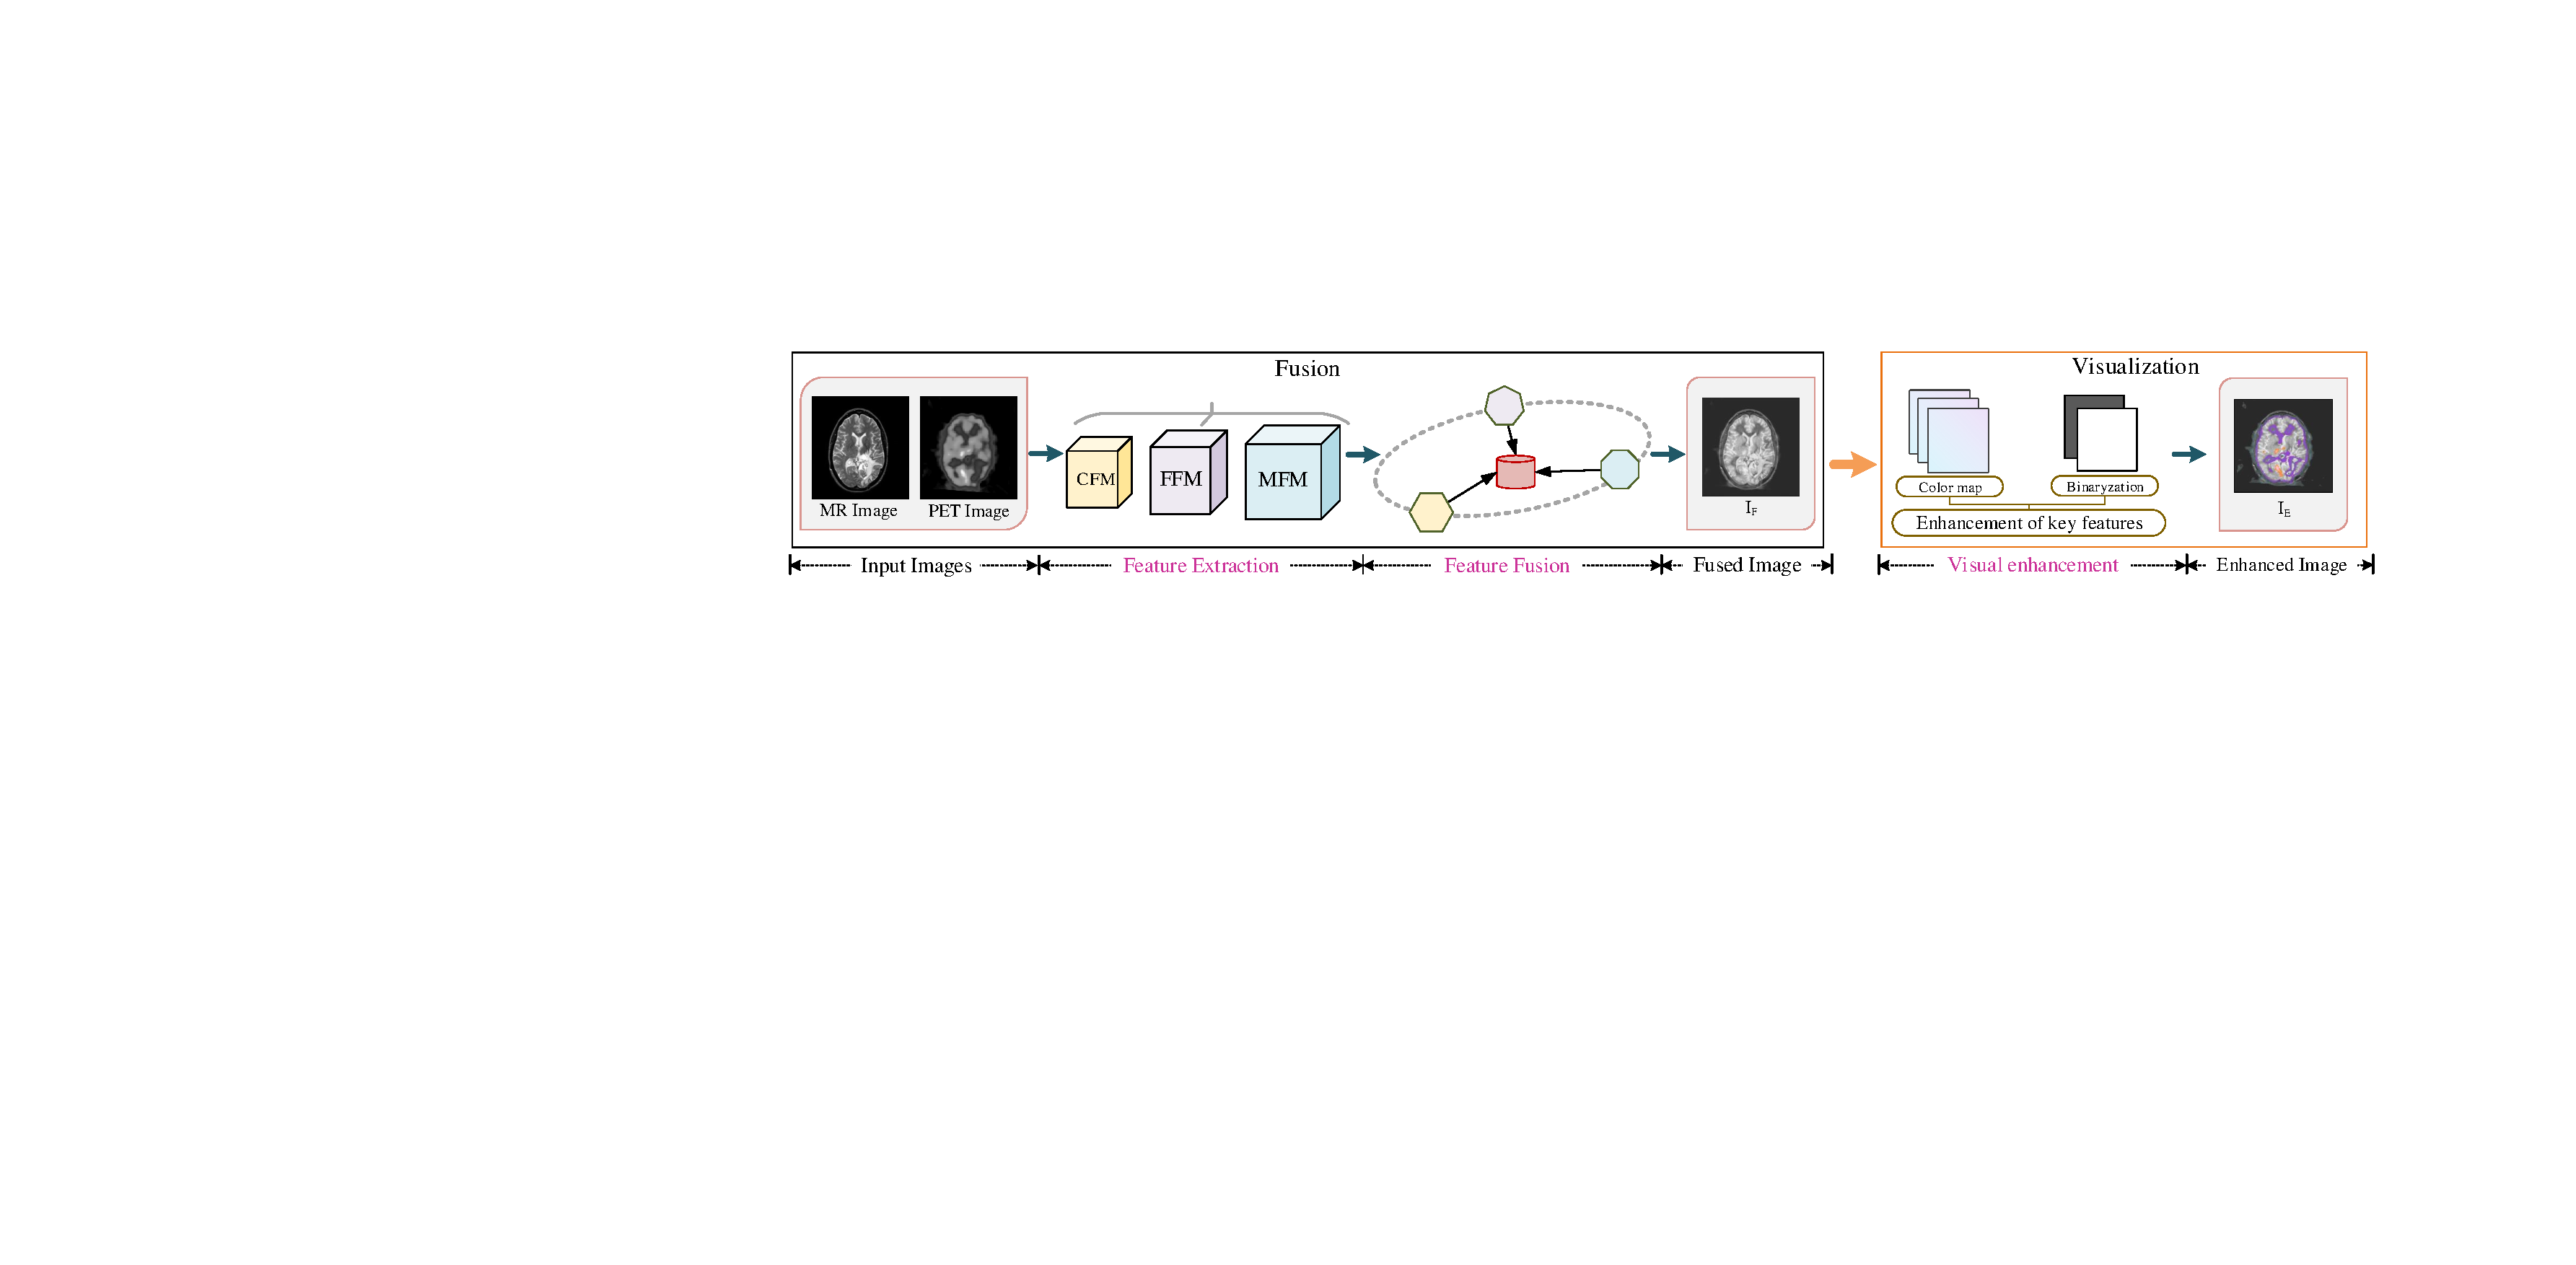
\includegraphics[width=0.97\linewidth]{figs/paper2Outline20230723.pdf}
      \caption{本小节提出的方法流程图(包括两个阶段:影像融合(图\ref{paper2framework})和可视化增强(图\ref{paper2visualization}))}\label{paper2flowchart}
    \end{figure*}

\subsubsection{多维度特征的提取策略}\label{chapter3.2:Feature_extraction}
为了从源影像中提取尽可能多的特征,本节采用多维度策略,充分利用空间和通道特征,建立了浅层特征模块(coarse feature module,CFM),深层特征模块(coarse feature module,FFM)以及多尺度特征模块(multi-scale feature module,MFM),分别提取浅层特征信息、深层特征信息以及多尺度特征信息。图\ref{paper2framework}中的蓝色虚线矩形表示特定的特征提取过程。其中,CFM为紫红色实线边缘黄底区域,FFM为蓝色实线边缘紫底区域,MFM为紫色边缘蓝底区域。在图\ref{paper2framework}中,不同的小方块代表三个步骤的组合(卷积运算,批量归一化和ReLU激活),不同颜色的方块代表不同大小的卷积核,黄色是1,蓝色是3,绿色是5,紫色是7,粉红色是3。不同大小的正方形表示不同的特征图大小和输出通道数。图\ref{paper2framework}右下角的灰色虚线框中有不同通道号的定义,即不同宽度的长方形代表不同通道的输出数量,并且颜色越深,通道的数量越大。对于输入影像,特征提取模块将获得三个维度的特征,即$CF_1$、$FF_1$和$MF_1$。 这些特征提取模块是根据人类视觉感知的感知特性和影像的物理特性设计的。

在图\ref{paper2framework}中,CFM由紫红色实线包围的黄色背景区域表示。CFM代表浅层特征模块,它负责通过卷积运算从影像中提取浅层特征。该模块利用较大的卷积核和较小的特征通道来捕捉影像的主要形状结构和边缘轮廓信息,代表影像背景和物体轮廓等全局低频信息。从图\ref{paper2framework}所示的特征图中,可以观察到,CFM模块提取的CF特征图表现出更清晰的轮廓。
类似地,在图\ref{paper2framework}中,FFM由蓝色实线包围的紫色背景区域表示。FFM指的是深层特征模块,它专注于深层特征提取。该模块采用较小的卷积核和较大的特征通道来捕获纹理细节,例如边缘,精细纹理细节和噪声,表示影像内具有显著变化的局部高频信息。用于深层特征提取的通道数远大于用于浅层特征提取的通道数。从图\ref{paper2framework}所示的特征图中,可以观察到由FFM模块提取的FF特征图显示了更明显的纹理细节。

在图\ref{paper2framework}中,MFM是紫色包围的蓝色背景的区域。MFM主要是从金字塔和分类的思想中获取影像的空间结构,从而获得多尺度影像之间的互补信息,利用多分辨率和多尺度影像之间的互补信息实现精细融合。在MFM中,还使用了深度分离卷积网络,便于挖掘更丰富有用的信息,为后续的影像理解和应用分析提供了良好的基础。另外,本节在构建网络时使用跳跃连接方法,与参考文献\cite{he2016deep,huang2017densely}一样。在本节的特征提取模块的设计中,更强调局部细粒度的信息,而不仅是全局特征。因此,使用短跳跃连接有利于局部信息的传输和保存,使网络能够更好地学习和利用这些局部化特征。因此,在特征提取过程中采用了短跳级联的方法,以获得更详细的信息,实现特征的逐步融合。

    \begin{figure*}[htbp]
      \centering
      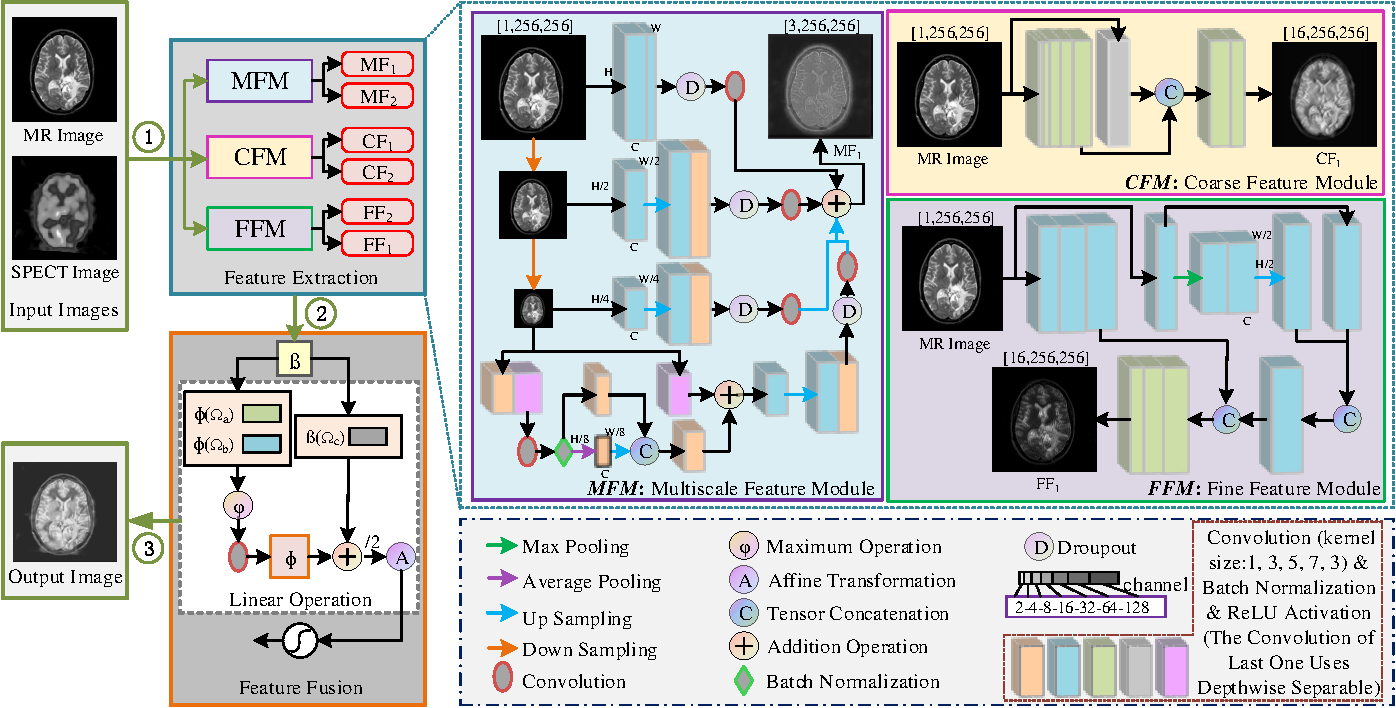
\includegraphics[width=0.9\linewidth]{figs/paper2framework.pdf}
      \caption{多模态影像融合网络的框架及具体的实现步骤}\label{paper2framework}
    \end{figure*}
\subsubsection{多维度特征的融合策略}\label{chapter3.2:Fusion_strategy}
MdAFuse从三个维度提取特征。浅层特征主要体现在边缘轮廓信息上,而深层特征则能保留纹理细节。为了从一幅影像中同时获得高频信息和低频信息,将每幅影像的粗特征和细特征相加,以获得具有更多信息的影像特征。为了突出两幅影像中的显著特征,特别是PET影像上的突出信息(通常对应于异常区域),本节使用最大值来获得更突出的部分。多尺度特征可以提供更多的结构信息,也可以补偿在跨尺度上丢失的局部细节。因此,浅层和深层特征必须是多尺度的。对于每个输入,将获得三个特征(CF、FF和MF)。那么,当输入两个模态影像时,共提取六个特征。并提出了一种自适应融合策略,使融合结果同时包含6个特征。本节设计的目标函数如(\ref{paper2tofuse}):
\begin{equation}\label{paper2tofuse}
   F=\delta(\Phi( (\upsilon (\varphi(\Phi(\Omega_a),~ \Phi(\Omega_b)) ) +\beta(\Omega_c))/2 )),
 \end{equation}
其中,$F$是融合的结果。 $\delta$ 是激活函数,本文采用$tanh$。$\Omega_a = \{ CF_1 \} \cup \{ FF_1 \}$, $\Omega_b = \{ CF_2 \} \cup \{ FF_2 \}$, $\Omega_c$ = $(MF_1+MF_2)/2$. 当计算$\Omega_a$的$\Phi$ 时,$\Gamma_1$和$\Gamma_2$分别表示$CF_1$和$FF_1$特征。类似地,如果计算$\Omega_b$的$\Phi$,$\Gamma_1$和 $\Gamma_2$分别表示$CF_2$和$FF_2$特征。
$\Phi$是通过仿射变换获得的两个特征之和,如等式(\ref{paper2F1})。在这个等式中,$U$表示特征图的大小。$A=Diag(B)$, $\beta(\Gamma)= A\Gamma(i)+e$, $B$和$e$是可学习参数。设置大小的规则与后归一化的规则相同\cite{2021Going}。 初始化$B$的值为1,$e$为0。 $\beta$是仿射变换函数,用于表示特征之间的相关性。在几何学领域,仿射变换被描述为一种结合了非奇异线性映射与平移的变换过程,它连接了两个向量空间并保持了它们的仿射结构,可用于保持二维影像之间的位置关系。因此,仿射变换被用作融合特征,以充分利用特征之间的相关性并保持它们。
 \begin{equation}\label{paper2F1}
\Phi(\Gamma)=\beta(\sum_{i=1}^{U}\Gamma_1(i))+\beta(\sum_{i=1}^{U}\Gamma_2(i))=A\sum_{j=1}^{2}\sum_{i=1}^{U}\Gamma_j(i)+2e,
 \end{equation}

$\upsilon$表示卷积运算,以保持输入和输出维度一致。$\varphi$是取最大值操作为突出显示重要信息。



\subsubsection{损失函数的构建}\label{chapter3.2:Loss_function}
为了更准确地重建源影像,在训练阶段考虑了特征提取阶段和融合过程,并获得了最小损失函数如式(\ref{paper2loss_function}):

 \begin{equation}\label{paper2loss_function}
   L=\alpha L_S +\beta L_M
   %L=L_S + L_M
 \end{equation}

同\ref{chapter3.1:MsgFusion}小节中的损失函数(\ref{paper1loss_function})设计相同,总损失函数由结构相似度$L_{S}$和像素损失$L_{M}$组成,具体计算同式(\ref{paper1L_{SSIM}})和(\ref{paper1L_{P}}):


在等式(\ref{paper2loss_function})中,$\alpha$和$\beta $是设置在区间$[0,1]$中的权重参数。通过对比分析,我将$\alpha $设为0.3,$\beta $设为0.7,结果最佳。在训练过程中,初始学习率为0.0001,60 epoch,批量大小为2,采用批量归一化,优化函数为Adam。

    \begin{figure*}[htbp]
      \centering
      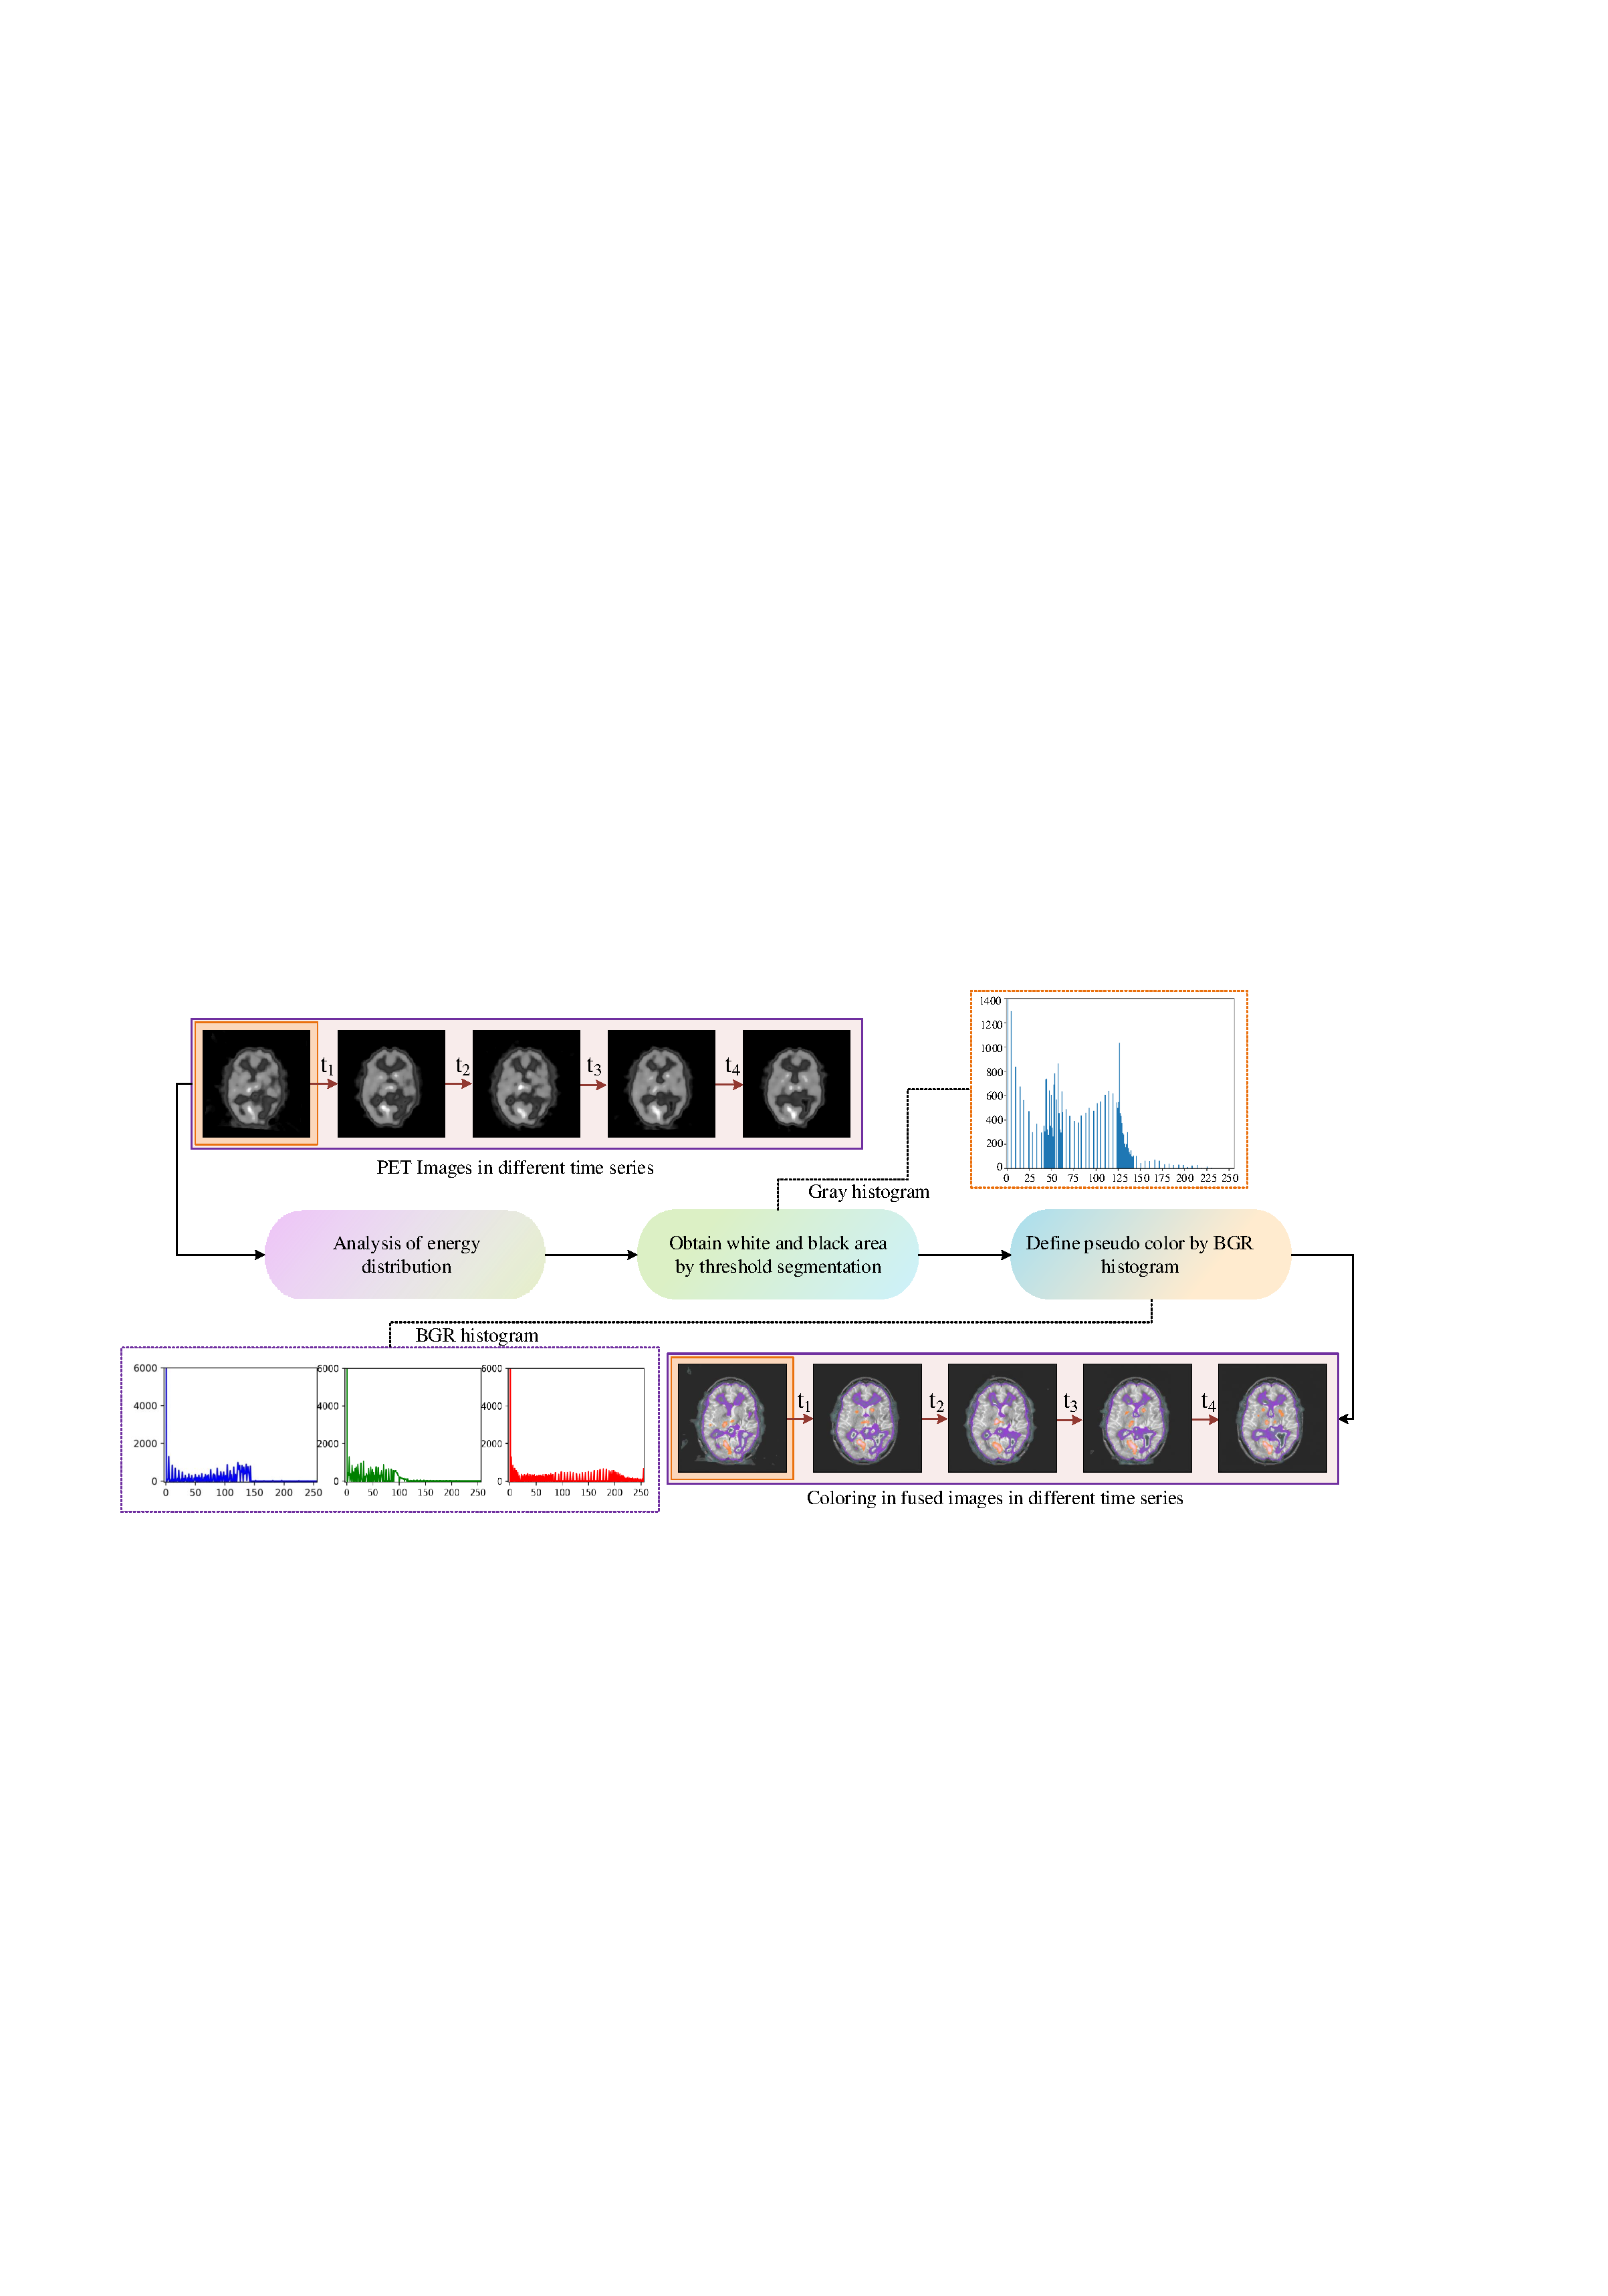
\includegraphics[width=0.9\linewidth]{figs/paper2visualization2023.pdf}
      \caption{增强融合影像中的关键特征策略}\label{paper2visualization}
    \end{figure*}
    
\subsubsection{关键特征的增强方案}\label{chapter3.2:Enhancement_of_key_features}
PET或SPECT影像的空间分辨率有限,边界灰度区分不清,限制了异常和正常区域的区分。为了提高可视性,伪彩色处理通常应用于临床环境,帮助医生识别边界细节并提高疾病诊断的准确性。


\begin{algorithm}[htbp]
\caption{Energy-based color enhancement}\label{paper2enhanceAlgorithm}
\centering
\begin{algorithmic}  [1]
    \Require Images $I_g$, $I_f$  
    \Ensure Image $I_e$
    
    \State $x \leftarrow $ the weight of $I_g$
    \State $y \leftarrow $ the height of $I_g$
    \State $\rho_w \leftarrow$ self-defined color for image of white area
    \State $\rho_b \leftarrow$ self-defined color for image of black area 
    \State $\eta_w,~ \eta_b \leftarrow$ $\gamma(I_g)$  %BinaryImage
    \State $\sigma \leftarrow$ \Call{\text{ColorUp}}{$I_g,~I_f,~ \eta_w,~ \rho_w$}
    \State $I_e \leftarrow$ \Call{\text{ColorUp}}{$I_g,~ \sigma,~ \eta_b,~ \rho_b$}
    %\State $I_e \leftarrow f_2$  
    %\State
    \end{algorithmic} 
    
\begin{algorithmic}[1]
\Function{ColorUp}{$I_g,~ I_f,~ I_a,~ I_c$}
   \State $I \leftarrow I_f.\text{copy}()$
        \If{$I_c == \rho_w$}
            \State $\quad \mu \leftarrow 5\sigma-20, ~\sigma=0,2,6,8$ %[-20,~ -10,~ 10,~ 20]
            \State $\quad \xi \leftarrow 5\iota-20,~0 \le \iota \le 4$
        \ElsIf{$I_c == \rho_b$}
            \State $\quad \mu \leftarrow 5\sigma-20,~0 \le \sigma \le 11 \&~\sigma\neq4$
            \State $\quad \xi \leftarrow 5\iota+10,~0 \le \iota \le 11$
         \EndIf
        \For{$i$=1 to $x$}
            \For{$j$=1 to $y$}
                \If{$I_a(i, ~j) \neq 0$}
                    \State $ a_{ij} \leftarrow I_a(i, ~j)$
                    \State $ \psi \leftarrow I_f(i, ~j) - I_g(i, ~j)$
                    \For{$k$=1 to  $(\text{len}(\mu))$}
                        \State $ I^{'}$  $\leftarrow I[a_{ij}]$
                        \State $ I_{c}^{'}$  $\leftarrow I_c[a_{ij}]$
                        \If{$\psi \leq \mu[k]$}
                            \State $\quad I^{'}(i, ~j) \leftarrow I_{c}^{'}(i, ~j) + \xi[k]$
                         \Else
                            \State $\quad I^{'}(i, ~j) \leftarrow I_{c}^{'}(i, ~j) + \xi[-1]$
                         \EndIf
                    \EndFor
                 \EndIf
            \EndFor
        \EndFor
      \State \Return $I^{'}$
\EndFunction
\end{algorithmic}
\end{algorithm}

在通过MRI-PET/SPECT融合生成灰度融合影像时,来自MRI的空间纹理是清晰的,而低分辨率灰度PET/SPECT影像难以揭示葡萄糖代谢的显著异常。现有的伪彩色方法涉及基于灰度的离散颜色映射和从灰度到颜色属性的连续转换。然而,这些技术中没有一种侧重于突出PET/SPECT影像中的这些显著异常。为了强调这些异常,基于PET/SPECT能量的灰度直方图,本节提出了一种颜色增强算法。该算法增强了异常信息的视觉效果,详细描述见算法\ref{paper2enhanceAlgorithm}和图\ref{paper2visualization}。


其中,$I_g$表示灰度PET/SPECT,$I_f$为融合的影像,$I_e$为增强的影像,$\eta_w$和$\eta_b$分别为阈值二值化过程中的白色和黑色区域。$\rho_w$和$\rho_b$是白色和黑色区域的两种自定义颜色。$I_c[a_{ij}](i,~j)$表示$I_c$中对应于$I_a$的区域。关键特征增强过程如图\ref{paper2visualization}所示。在这部分工作中,主要目的是获得可以代表葡萄糖含量或生理代谢的PET/SPECT影像和增强融合结果中的重要信息。


首先,分析灰度PET/SPECT影像中的能量分布,包括不同像素的大小分布、不同位置像素的分布、有用信息的集中区域以及代表相似信息的区域数量。在PET/SPECT中主要存在两种形式的能量分布。一种是葡萄糖含量高或代谢旺盛的组织,显示在白色区域。另一种是葡萄糖含量低或代谢弱的组织,用黑色区域表示。其次,需要在灰色PET/SPECT中获得黑色和白色区域。使用阈值法来提取这两种类型的影像。阈值化的关键在于阈值的设置,$\tau_w$是提取白色区域块的阈值,其由等式(\ref{paper2Tw})获得,$\zeta$是指直方图中峰值的灰度值,$\kappa$表示指峰的总数。在公式(\ref{paper2Pks})中的函数表示直方图的计算,$\phi$表示其转换到一维的操作。参数$\chi$表示峰与其周围谷之间的最小高度差,在图\ref{paper2visualization}的示例中设置为100。$\vartheta$的作用是寻找直方图中的峰值。对于黑色区域,设置了两个阈值。为了消除一些噪声并避免假溢出,添加另一个阈值$\tau_{b1}$,其被设置为10。$\tau_{b2}$是通过Otsu方法获得的全局阈值。算法1中的$\gamma$表示白色特征和黑色特征的两个二值影像,这两个二值影像是由公式(\ref{paper2Ia})和(\ref{paper2Ib})分别的计算获得。在式(\ref{paper2Ia})和(\ref{paper2Ib}),$I_{g}(i,~j)$表示影像$I_{g}$中第$i$行第$j$列的位置处的像素值。
 
\begin{equation}\label{paper2Pks}
\zeta =\vartheta\left(\chi\left( \phi \left(I_g\right)\right), ~p\right) ,
\end{equation}
\begin{equation}\label{paper2Tw}
%\tau_w =P_{k s}\left[N_{k s}-1\right] 
\tau_w =\zeta^{l},~ l=\kappa-1,
\end{equation}
\begin{equation}\label{paper2Ia}
\begin{aligned}
I_{w}(i,~ j)=\begin{cases}
0,  & I_{g}(i,~ j)\le \tau_w\\
255,  & I_{g}(i,~ j)>\tau_w\\
\end{cases} \\
\end{aligned},
\end{equation}
\begin{equation}\label{paper2Ib}
\begin{aligned}
I_{b}(i,~ j)=\begin{cases}
0,  & I_{g}(i,~ j)< \tau_{b1} ~\|~ I_{g}(i,~ j)>\tau_{b2}\\
255,  & I_{g}(i,~ j)>\tau_{b1} ~\&~ I_{g}(i,~ j)\le \tau_{b2}\\
\end{cases} \\
\end{aligned},
\end{equation}


最后,根据BGR直方图定义伪彩色,具体过程如算法2所示,在图\ref{paper2visualization}中包含三幅影像的直方图(根据伪彩色PET/SPECT影像计算的相应BGR的三种颜色的直方图)。为了便于观察,纵轴的值仅小于6000。从BGR直方图中,可以确定蓝色、绿色和红色像素值的大致范围。因此,白色区域呈现黄色显示,黑色区域呈现深蓝色显示。$\rho_w$和$\rho_b$分别用于表示黄色和深蓝色区域。亮度根据像素的大小而变化,并且对于没有辅助诊断的区域不显示颜色。然后,将融合影像与原始PET/SPECT灰度影像之间的像素值进行比较,并做出相应的改变。具体过程如算法\ref{paper2enhanceAlgorithm}的$ColorUp$所示,以及得到的影像的着色效果如图\ref{paper2visualization}所示。


\subsection{多模态影像融合的实验}
本节使用Python 3.7.9和Pytorch版本1.7.1+cu110及其相应的CUDA版本11.1。GNU/Linux x86,GeForce RTX 3090 Ti GPU 20GB RAM-64系统。在训练过程中,使用的数据来自ADNI(https://adni.loni.usc.edu/data-samples/access-data/),本节下载了555个MRI和PET影像对。样本的年龄从55岁到90岁不等,样本的性别有男有女。所有影像均作为轴向切片进行分析,体素尺寸为1.0$\times$1.0$\times$1.0 $mm^{3}$。通过非相交数据集测试对本节的训练模型进行交叉验证。
从ADNI和全脑图谱(http://www.med.harvard.edu/AANLIB/home.html.)中获得了80个独立不重复受试者的137个影像对进行测试。其中,74对MRI-SPECT,42对MRI-PET,21对MRI-CT。在图\ref{paper2d2roi}和图\ref{paper2029_1_roi}的融合实验中,测试数据是具有胶质瘤的MRI和SPECT脑影像,这是脑神经系统中的典型应用。MRI与PET/SPECT的融合可以整合生物解剖信息和生理代谢信息,帮助医生对病变进行定位和诊断。实验中还分析和比较了现有的几种基于传统方法和深度学习方法的融合算法。

为了定量衡量不同融合方法的融合效果,本节采用了9种质量评价指标,信息熵(EN)\cite{2008Assessment},互信息(MI)\cite{2005Feature},标准差(SD)\cite{Yun1997In},视觉信息保真度(VIF)\cite{2013A},结构相似性(SSIM)\cite{wang2004image},差异相关性之和(SCD)\cite{Aslantas2015A},相关系数(CC)\cite{han2008study},均方误差(MSE)\cite{willmott2005advantages}和空间频率误差比(rSFe)\cite{2007A}。对于MSE,较小的值表示更好的性能。对于rSFe,其较小绝对值对应于较好的融合效果。而其他七个评价指标则相反。rSFe是一个相对不常见的评价指标,用于衡量影像的整体活动水平,它由像素点中的四个空间频率(行、列、主对角线、次对角线)和四个方向的一阶梯度值(水平、垂直、主对角线、次对角线)整合而成,其数值绝对值越小,则表明融合效果越佳。为了便于比较和分析,本节对部分指标的计算结果进行了归一化处理。如表\ref{lineTransformation}所示,本节对每个度量执行线性变换,其中$k_i$和$b_i$ ($i=1, 2, 3$)分别表示图\ref{paper2d2_10roi_value}、图\ref{paper2029_1_roi_value}和图\ref{paper2ablation_value1}中的变换系数。

\begin{table}[ht]
%\small
\centering
  \caption{每个度量指标值上的线性变换,其中$k_i$和$b_i$ ($i=1, 2, 3$)分别表示图\ref{paper2d2_10roi_value}、图\ref{paper2029_1_roi_value}和图\ref{paper2ablation_value1}中的变换系数}\label{lineTransformation}
\begin{tabular}{cccccccccc}
\hline
\textit{\textbf{}} & \textbf{EN} & \textbf{MI} & \textbf{SD} & \textbf{VIF} & \textbf{SCD} & \textbf{SSIM} & \textbf{CC}  & \textbf{MSE} & \textbf{rSFe} \\ \hline
$k_1$                 & 8           & 6           & 1/2.1     & 48           & 29  & 16   & 42  & 18  & -37  \\
$b_1$                 & -11         & 0           & 0           & 0            & 2   & 0    & 5   & 5   & 8    \\
$k_2$                 & 5.6         & 5           & 0.4         & 31           & 18  & 16   & 26  & 240 & -32  \\
$b_2$                 & 0           & 0           & 0           & 0            & 0   & 0    & 0   & 3   & 6    \\
$k_3$                 & 1           & 1           & 1/13     & 5            & 2   & 10   & 100 & 15  & -8   \\
$b_3$                 & -1          & 0           & 0           & 0            & 0   & -14  & 90  & 0   & 0    \\
\hline
\end{tabular}
\end{table}

\subsubsection{与传统方法的实验对比分析}
在本小节测试了三种传统的融合方法,并将它们与本节提出的方法进行了比较。如图\ref{paper2d2roi}所示,第一列和第二列分别显示来自具有脑异常的一些病例的MRI和SPECT源影像。以下各列显示了通过三种传统方法和建议方法获得的结果,每种方法各一列。在图\ref{paper2d2roi}中,可以观察到来自不同融合方法的融合影像之间的差异。PCF是一种利用小波变换原理实现影像融合的方法,融合后的影像信息丢失严重。LatLrr是一种低秩表示方法,其融合策略是简单的加权平均。这种方法的结果可以保持良好的纹理细节,但较少的SPECT影像的信息。atsIF(自适应双尺度影像融合)\cite{2020An}是一种通过颜色空间转换的融合策略,可以保留更多的SPECT信息,但MRI细节丢失。与其他方法相比,本节提出的方法可以更好地保持两个源影像的信息。在第一行中,每个影像的三个局部区域使用三个彩色正方形包围并被放大,并分别显示在第二,第三和第四行中,以进行更清晰的比较。

   \begin{figure}[ht]
      \centering
      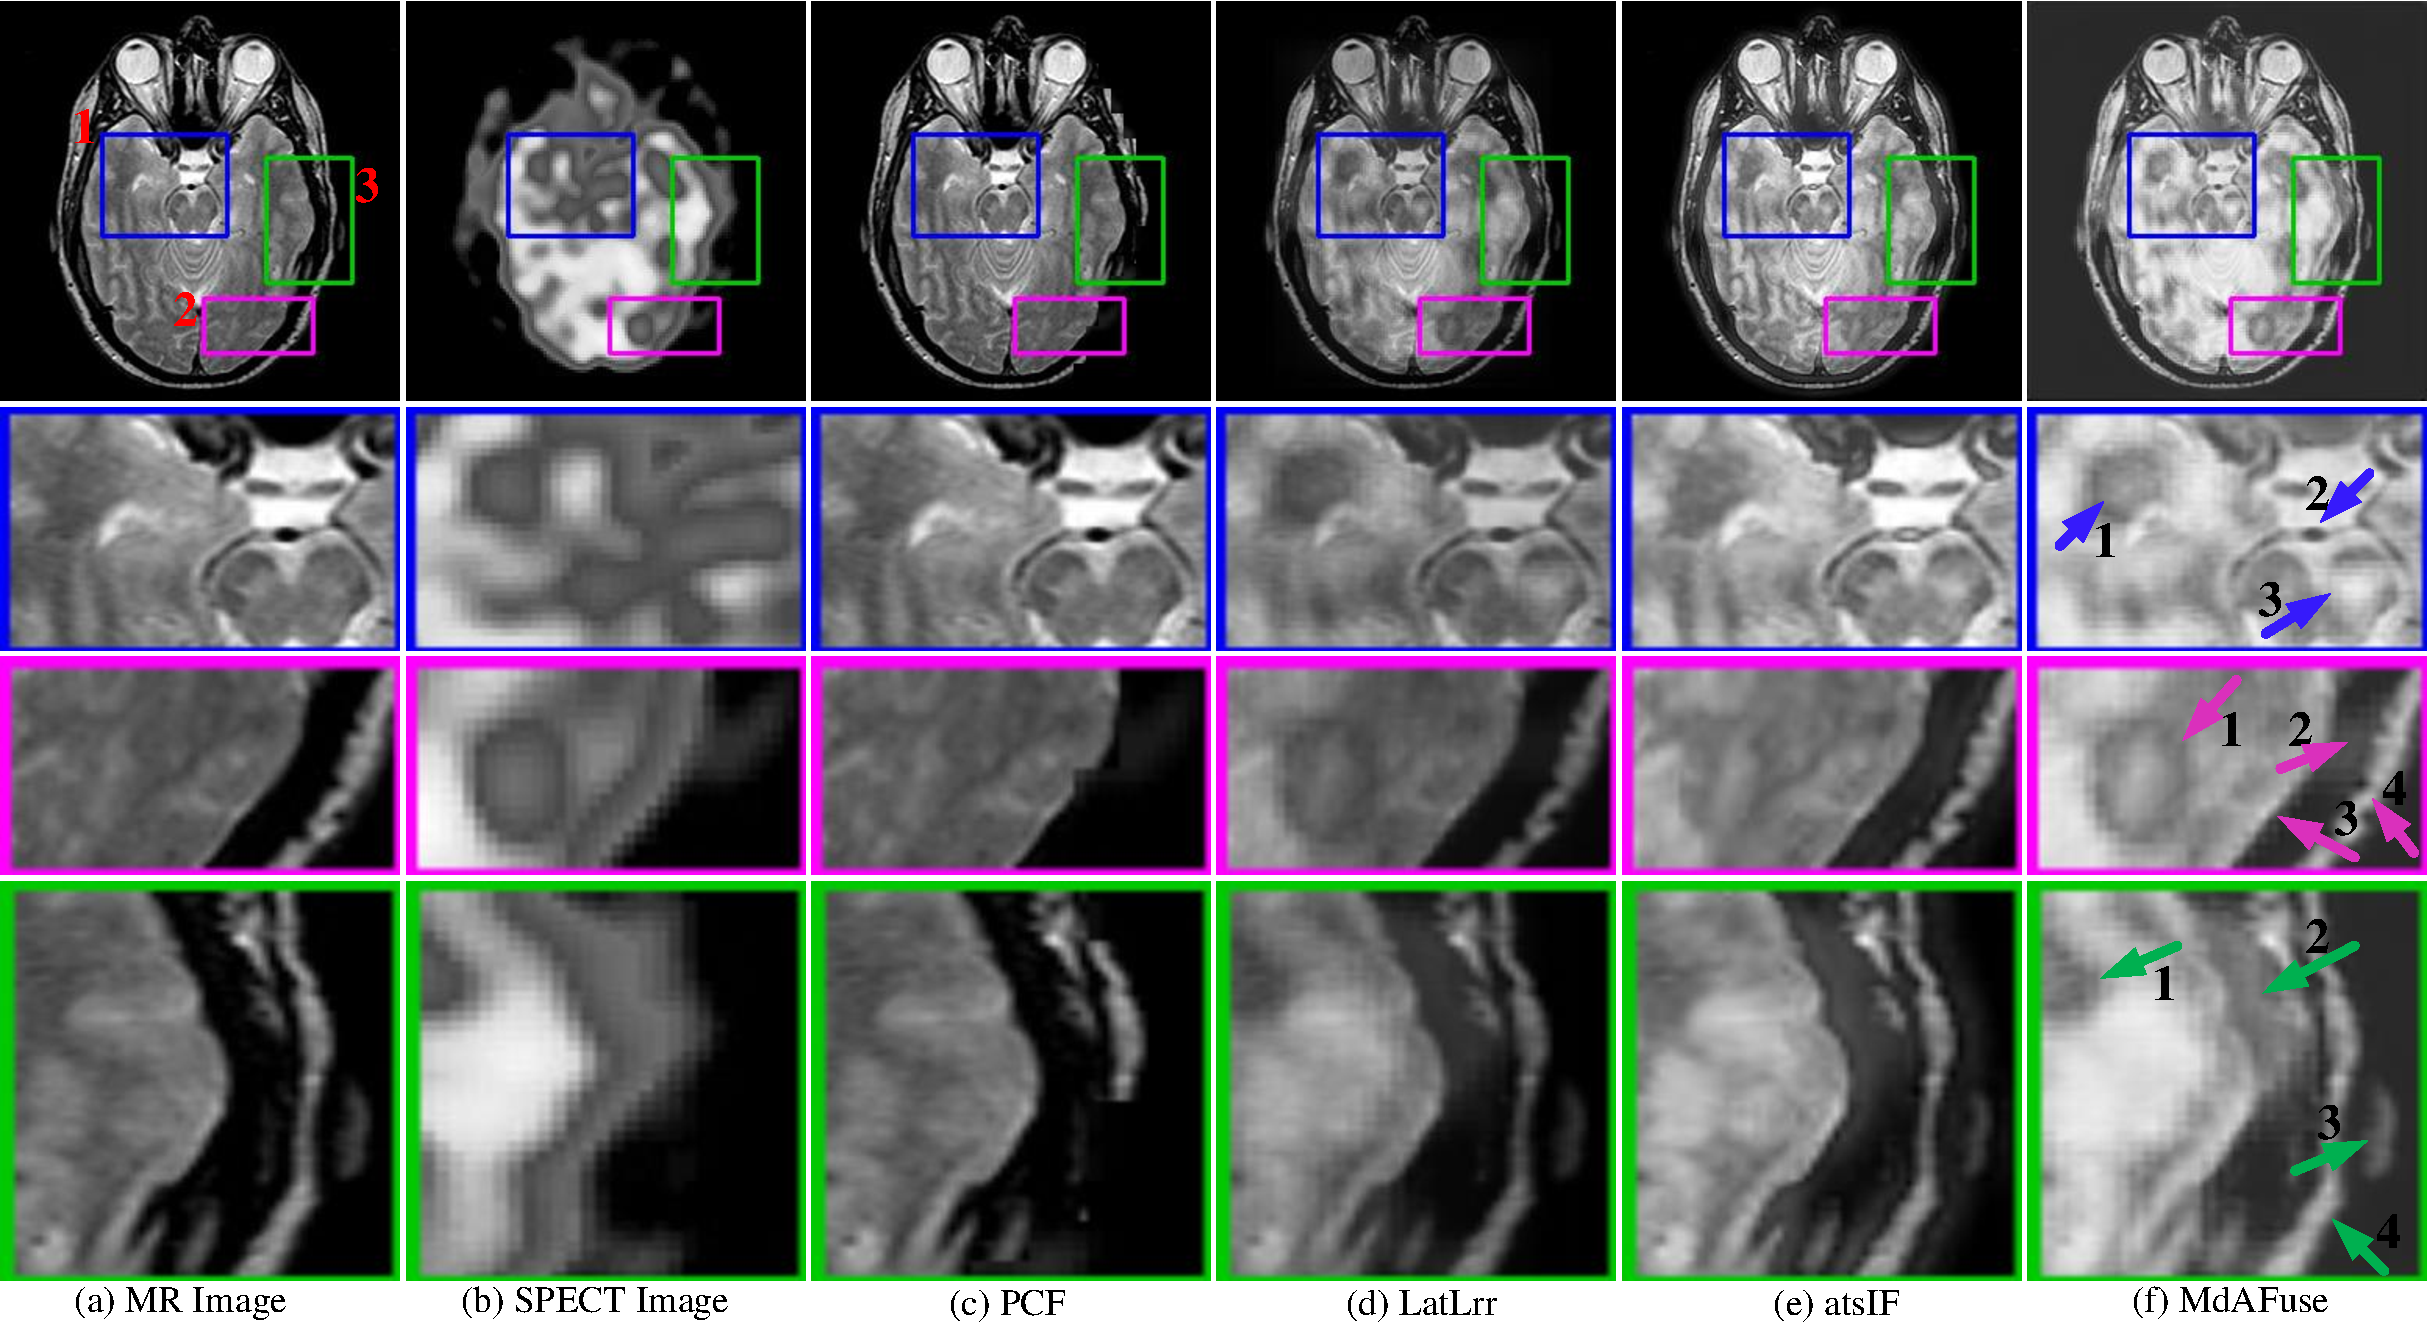
\includegraphics[width=0.9\linewidth]{figs/paper2d2_10_roi.pdf}
      \caption{比较传统的融合方法和本节提出的MdAFuse方法的MRI-SPECT融合结果}\label{paper2d2roi}
    \end{figure}
图\ref{paper2d2roi}中的第二行列出了与第一行中蓝色正方形内的部分相对应的放大影像。在最后一列,本节用三个箭头标记了颞叶、基底动脉和脑桥。颞叶在MRI上呈灰色,不规则。SPECT显示较浅的灰色圆圈,具有明显的色差。在PCF结果中,该区域不明显,MRI上的特征完全保留,但SPECT上没有。在LatLrr融合的结果中,该区域可以保留两个源影像的信息,但也丢失了部分SPECT信息,例如颞叶周围的像素值,这是没有区别的。atsIF方法的效果在亮度方面有了很大的提高,可以在SPECT中保留更多的信息,但合并后的源影像会出现信息丢失。与其他方法相比,本节提出的方法可以很好地保留颞叶区域的特征。对于基底动脉区,也注意到明显的差异。在MRI中,该区域是一个小的黑色椭圆,而在SPECT中,它是一个均匀的灰色区域,没有形状特征。PCF完全保留了MRI上的信息,LatLrr和所提出的方法显示该位置区域为深灰色,形状没有改变。atsIF的融合结果变成了一个白色区域,在小椭圆的外面有一个黑色的圆圈很明显。箭头3指向脑桥区,这是MRI上灰度分布不均匀的区域,SPECT影像上亮度明显且类似三角形的小区域。同样,在PCF的融合结果中找不到SPECT的特征信息,在LatLrr和atsIF结果中该位置区域的亮度信息也不明显。相对而言,本小节提出的方法的结果能清晰地反映MRI和SPECT的特征。

图\ref{paper2d2roi}中的第三行列出了与第一行中紫色方块内的区域相对应的放大影像。同样,在最后一列中,标记了指向枕叶、枕骨、侧窦和枕叶轮廓的四个箭头。从四个箭头的显示也证明了该方法的融合效果更好,尤其是在第一个箭头区域。图\ref{paper2d2roi}中的第四行列出了与第一行中蓝色方块内的部分对应的放大影像。最后一列中的四个箭头指向颞叶、颞肌、耳廓和外侧枕骨。从四个箭头的显示也证明了本小节方法的融合效果更好。

    \begin{figure}[ht]
      \centering
      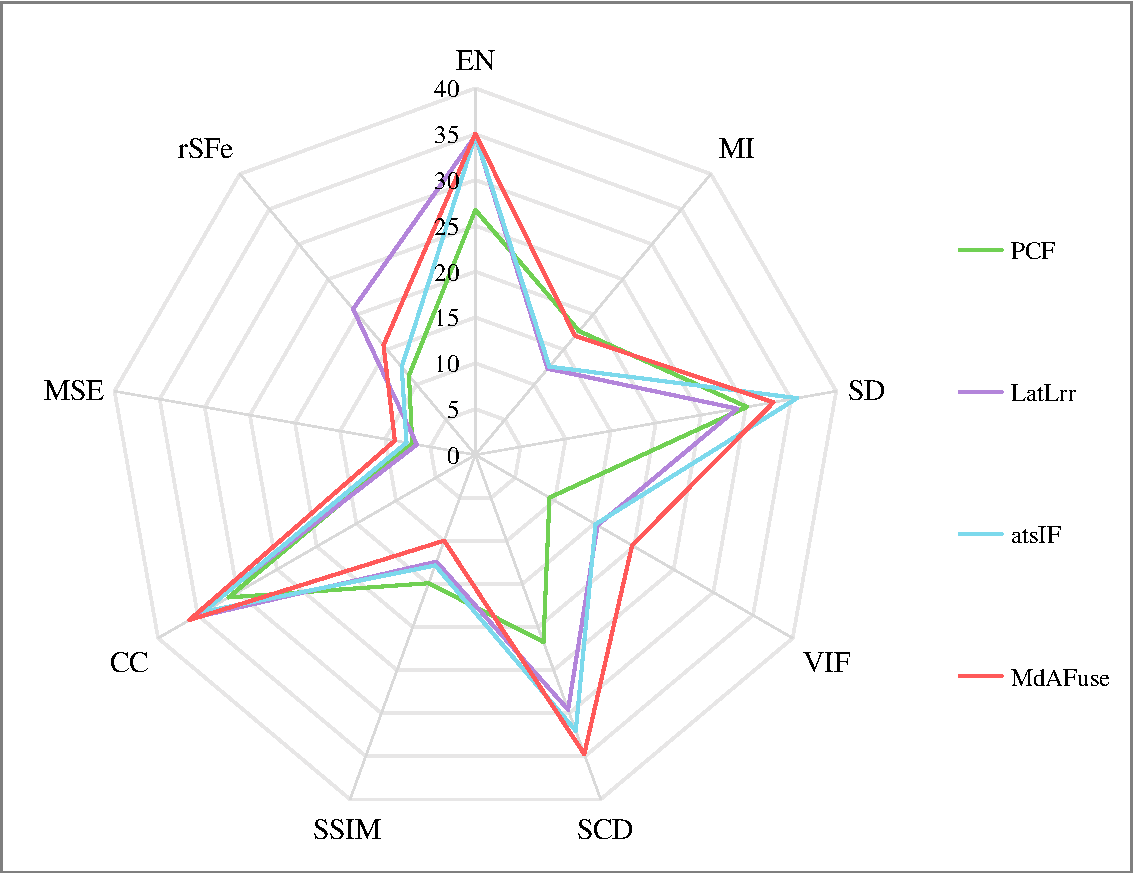
\includegraphics[width=0.9\linewidth]{figs/paper2traditionMetrics2024.pdf}
      \caption{图\ref{paper2d2roi}中与基于传统医学影像融合方法的客观评估比较分析}\label{paper2d2_10roi_value}
    \end{figure}

传统的影像融合方法主要属于像素级的融合操作,这种方法追求的是最大限度地保留信息。为了充分验证所设计的影像融合模型的实际效能,使用9个度量(EN,MI,SD,VIF,SSIM,SCD,CC,MSE,rSFe)来评估融合结果的质量,如图\ref{paper2d2_10roi_value}所示。在图\ref{paper2d2_10roi_value}中,可以观察到本节的MdAFuse方法的大多数度量都具有优势。具体地,SCD值比次优值高9\%。


\subsubsection{与新型方法的实验对比分析}
在这一部分中,对几种基于DL的影像融合方法进行了实验,并对它们的融合结果进行了比较。如图\ref{paper2029_1_roi}所示,第一列和第二列示出了要融合的MRI和SPECT源影像,并且随后的6列展示出了通过6种融合方法(包括所提出的方法:MdAFuse)获得的融合结果。从这些结果中,可以观察到不同的融合方法之间的差异。总体而言,可以观察到U2Fusion和CDDFused生成的融合影像似乎没有考虑SPECT的信息。虽然FusionDN和DeFusion方法保留了源影像中的SPECT信息,但仍然可以观察到一些信息丢失。FunFuseAn方法的影像融合效果相对较好,与本文提出的MdAFuse方法在视觉上具有相似性。因此,放大了三个小区域,以进一步比较和分析。在第一行中,使用三种颜色标记三个不同的区域并将其放大,如第二至第四行所示。



 \begin{figure}[ht]
      \centering
      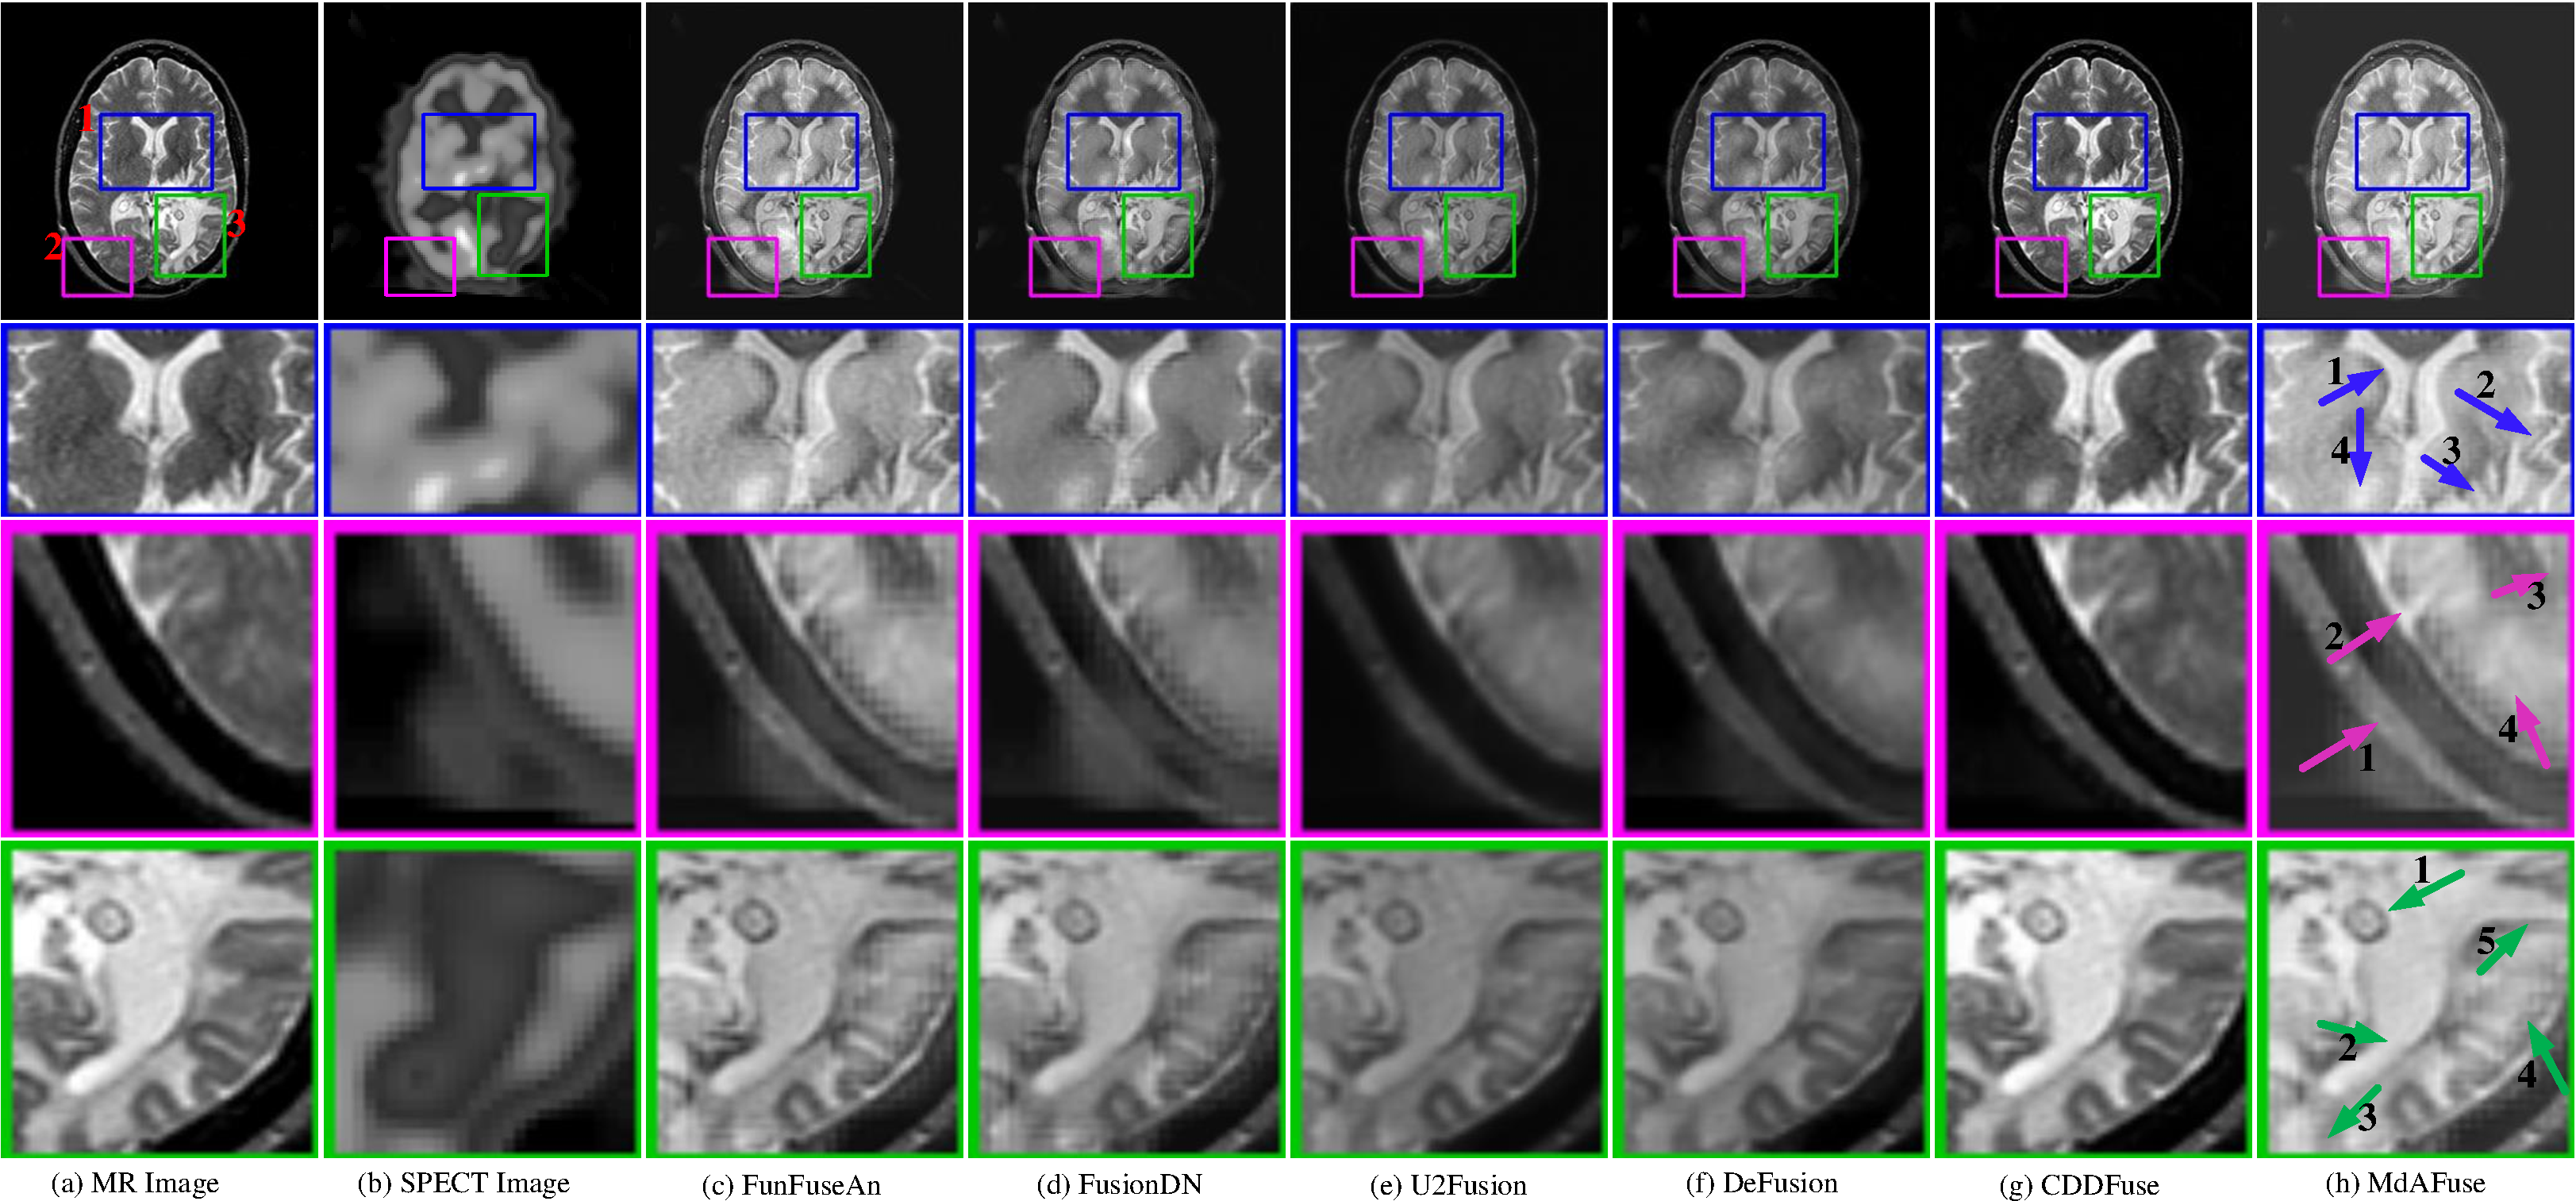
\includegraphics[width=0.9\linewidth]{figs/paper2_29_1_roi2024.pdf}
      \caption{本节提出的MdAFuse方法与现有的基于DL的方法性能比较}\label{paper2029_1_roi}
    \end{figure}

首先,图\ref{paper2029_1_roi}中蓝色方块标记的ROI主要反映侧脑室前角、丘脑和颞叶的信息。在MRI中,侧脑室的前角呈白色且对称,而在SPECT影像中,左侧脑室是灰色的。左侧丘脑区域在MRI中为深灰色,而晶状体区域在SPECT影像中为明亮。右侧丘脑区域呈白色,在MRI中看起来像丛林,而在SPECT影像中,它呈黑色,不规则。颞叶的面积在蓝色方块的左右两侧测量,主要反映在MRI上,是连续的。在图\ref{paper2029_1_roi}的最后一列中,四个区域用彩色方块标记。区域1为侧脑室左前角。
U2Fusion和DeFusion中这个位置的结构相对完整,但影像看起来模糊。CDDFuse突出显示MRI信息。FunFuseAn类似于FusionDN,两者都有色差。侧脑室左前角FusionDN较完整,而侧脑室右前角像素值分布不均匀。相比之下,MdAFuse可以更完整地保留MRI特征。区域2是颞叶。在FunFuseAn和FusionDN的结果中,结构相对完整和连续,但颜色相对较暗。U2Fusion和DeFusion的结果可以很好地保留MRI特征,但存在伪影。区域3是丘脑右侧的位置,在MRI上应该反映更多的纹理细节。在U2Fusion和DeFusion的结果中,位置不明显。FunFuseAn、FusionDN和CDDFuse很相似,组织结构不完整。相比之下,MdAFuse可以完全保留右侧丘脑。区域4为左侧丘脑,应显示一个亮点的扩散区。FusionDN和DeFusion的结果显示无明显状态。U2Fusion的结果可以识别出一个亮度块,但该区域的灰度值比较均匀,没有发现差异变化;其他方法可以明显地发现亮度块,可以检测出更多层次的亮度特征。

   \begin{figure}[htb]
      \centering
      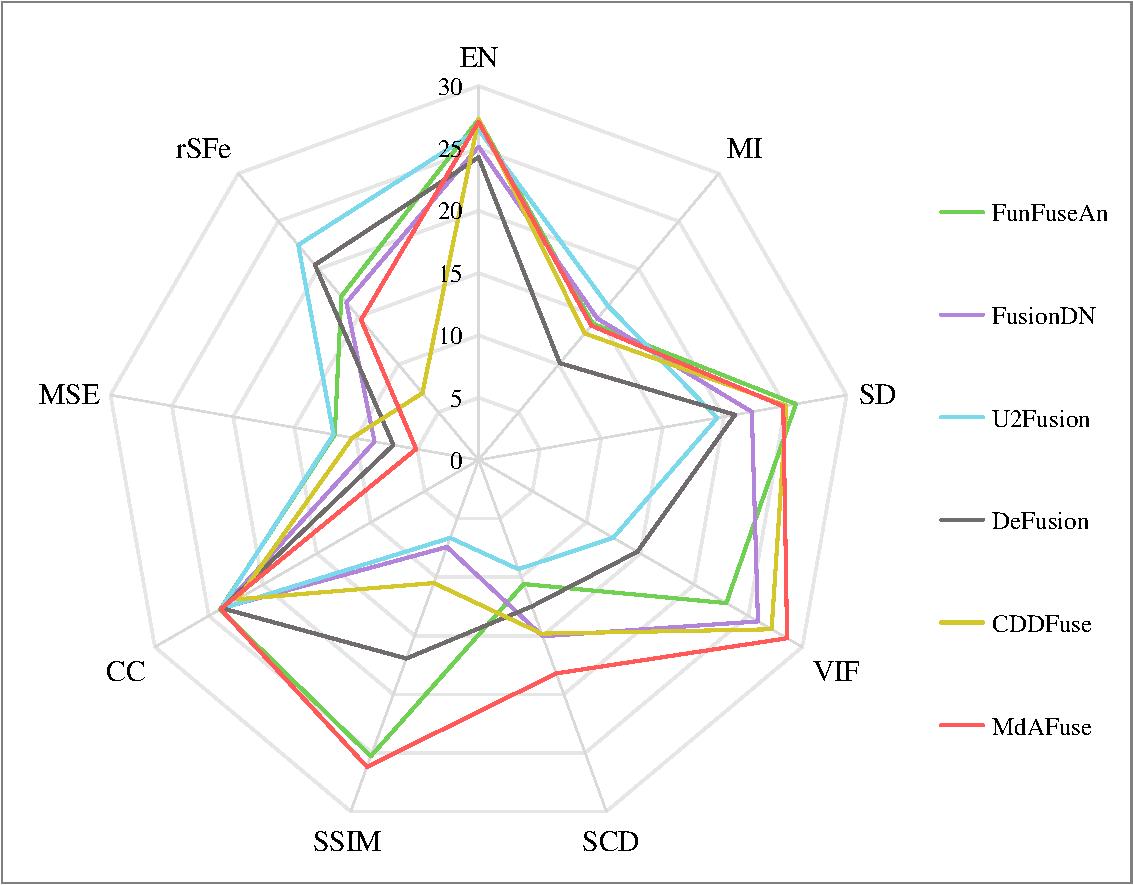
\includegraphics[width=0.9\linewidth]{figs/paper2DLMetrics2024.pdf}
      \caption{图\ref{paper2029_1_roi}中与基于DL医学影像融合方法的客观评估比较分析}\label{paper2029_1_roi_value}
    \end{figure}

其次,在图\ref{paper2029_1_roi}中放大的第二个紫色方块中,最后一列标记的四个区域是脑膜、枕叶、侧脑室枕角和大脑皮层(灰质)。在MRI中,ROI 1显示为粗灰色柱,而SPECT影像显示不均匀的波浪状灰色块。FusionDN和DeFusion的结果都显示出一些丢失,并且没有保留MRI的完整结构信息。U2Fusion和CDDFuse主要保留MRI信息,忽略SPECT特征。相比之下,FunFuseAn和MdAFuse考虑到了两幅原始影像中更重要的信息,并更完整地保留有用的特征。ROI 2是枕叶,在U2Fusion和DeFusion结果中不容易找到其。在FusionDN的结果中,未观察到位置区域与周围区域之间的显著差异。ROI 3是侧脑室的左枕角。可以在MRI上找到枕角的特征信息,这是SPECT影像上灰度值均匀的区域。FunFuseAn可以发现细微的变化,但本节的方法的结果更明显。箭头4指的是大脑皮层的一部分(灰质)。在这一区域的MRI中,可以发现一个灰度值分布不均匀的散在区域,并且可以观察到精细的纹理特征。在SPECT影像中,该区域是具有均匀灰度值的浅灰色。从测试结果来看,只有FunFuseAn和MdAFuse的灰度值层次结构比较突出,能够比较完整地保留MRI的特征信息,而其他方法的灰度值层次结果都难以识别。

最后,对于图\ref{paper2029_1_roi}中第三个蓝色正方形区域,信息量丰富,包括脉络丛、侧脑室枕角、枕叶、岛叶和小脑。五个箭头指向本节的方法的结果,这是明显不同于其他方法。区域1是脉络丛。在MRI中,整个位置是两个灰色同心圆。外圆的灰度值比内圆的灰度值深,差异明显。圆心的灰度值仅次于外圆,也比较突出。在SPECT影像中,灰度值更均匀。U2Fusion和DeFusion的结果显示,内圆的半径相对较大,圆心不明显,内圆区域的像素值没有差异。FunFuseAn,FusionDN,CDDFuse和本节的MdAFuse方法可以更好地保留MRI信息,并且可以清楚地找到内圈和外圈以及圆心之间的明显差异。类似地,其他箭头指向在本节的MdAFuse方法中获得更好的效果。

基于深度学习的融合方法主要可以从它们在特征级的操作来区分,同样地使用9个质量评估度量(EN、MI、SD、VIF、SSIM、SCD、CC、MSE、rSFe)来评估融合影像结果的质量,如图\ref{paper2029_1_roi_value}所示。从图\ref{paper2029_1_roi_value}中,可以观察到,与其他方法相比,本节的方法在6个指标上具有优势,特别是在SSIM,SCD,VIF和MSE中,与次优值的差异非常明显。对于rSFe度量,CDDFuse方法的值最小,但这个相对较小的值似乎有点异常。这可能是由于其较少保留SPECT影像中的信息,如图\ref{paper2029_1_roi}(g)所示。相比之下,本节的方法在这个指标上表现得更好。虽然在SD和MI指标上的表现并不突出,但与最大值和第二大值的差距并不明显。


    \begin{figure}[htbp]
      \centering
      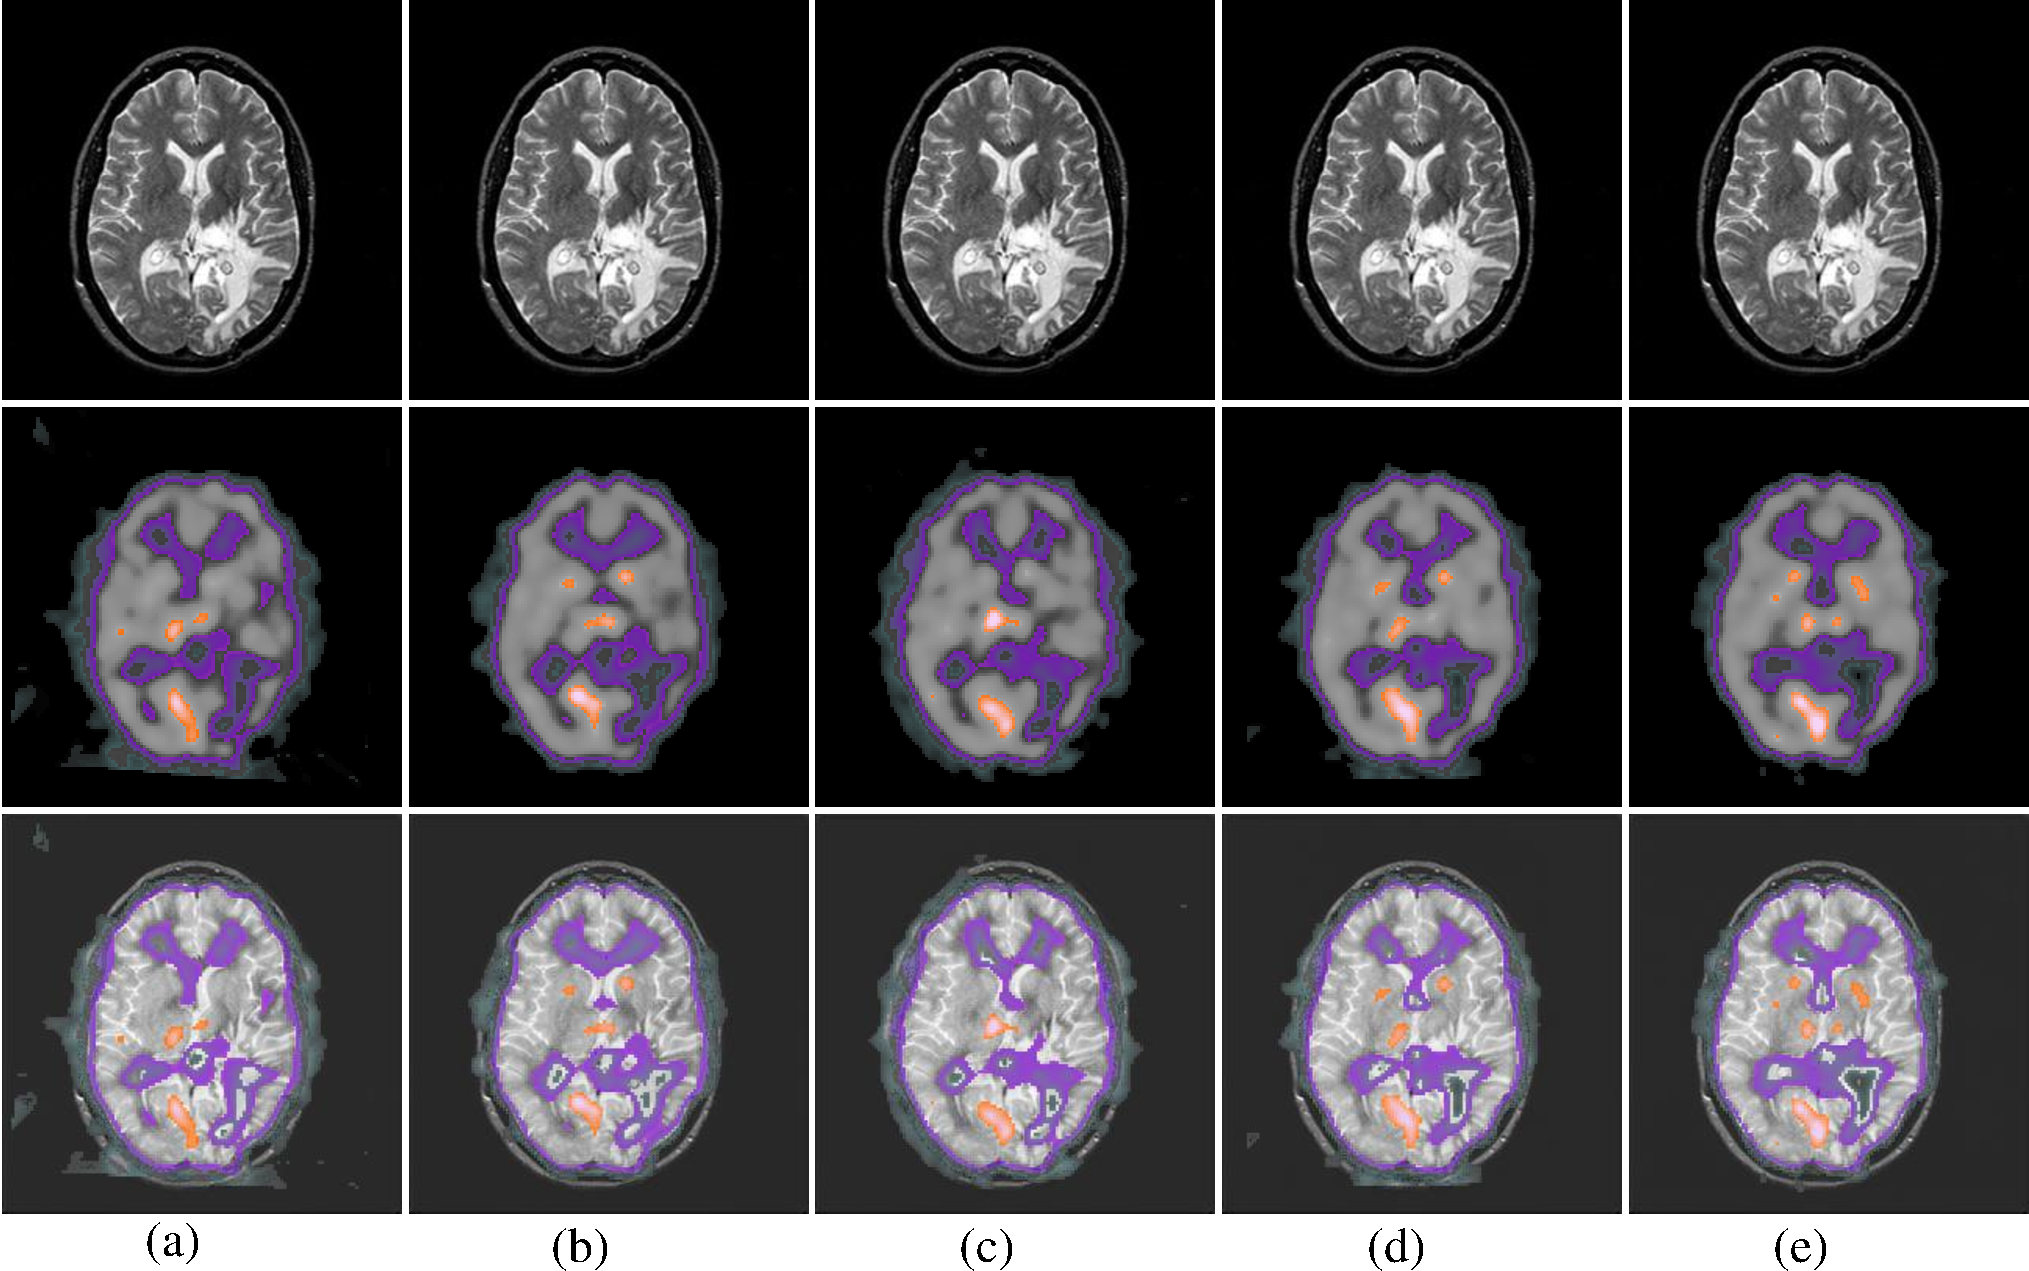
\includegraphics[width=0.9\linewidth]{figs/paper2029color.pdf}
      \caption{增强某一受试者融合影像中的关键特征}\label{paper2029_color_i}
    \end{figure}

采用74对MRI-SPECT、42对MRI-PET和21对MRI-CT医学影像融合结果与几种SOTA方法的定量分析结果见表\ref{paper2quantitativeMetrics}。表中的值表示每种方法在各种度量中的平均性能。在表\ref{paper2quantitativeMetrics}中,以粗体显示的值表示最佳值,而那些带下划线的值表示次优值。总体而言,本节的MdAFuse方法优于其他方法,在大多数指标中显示出上级结果,特别是在EN、VIF、SSIM和MSE上。CDDFuse是目前最先进的方法,当应用于MRI-SPECT融合时,本节提出的方法在VIF和SSIM中分别获得了11.14\%和18.38\%的提升。此外,本节提出的方法将MSE降低了2.63\%。在MRI-PET融合的情况下,本节的方法使得VIF和SSIM分别提高了13.76\%和5.61\%,而MSE降低了4.50\%。

\begin{table*}[htb]
\centering
  \caption{多模态医学影像融合结果与SOTA方法的定量比较与分析}\label{paper2quantitativeMetrics}
  \scriptsize
\begin{tabular}{cccccccccc}
\hline

\textit{MRI-SPECT} & \textbf{EN}     & \textbf{MI}     & \textbf{SD}      & \textbf{VIF}   & \textbf{SCD}    & \textbf{SSIM}   & \textbf{CC}     & \textbf{MSE}    & \textbf{rSFe}    \\ \hline
FunFuseAn                  & \underline{4.2348}    & \underline{2.6155}          & 55.3604          & 0.8947          & 1.0452          & \underline{ 1.5794}    & \textbf{0.8917} & 0.0535          & -0.3340          \\
FusionDN                  & 3.9001          & \textbf{2.6912} & 56.5726          & 0.5216          & 0.9051          & 0.4167          & 0.8756          & 0.0388          & -0.2623          \\
U2Fusion                        & 4.0581          & 2.4404          & 42.2308          & 0.3188          & 1.7674          & 0.3016          & 0.8832          & 0.0344          & -0.5399          \\
DeFusion                       & 3.7698          & 1.7543          & 49.9900          & 0.5393          & 0.7180          & 1.4480          & 0.8654          & \underline{ 0.0225}    & -0.3775          \\
CDDFuse                    & 3.9151          & 2.4925          & \textbf{58.3698} & \underline{ 0.9666}    & \underline{ 1.3458}    & 1.4717          & 0.8381          & 0.0375          & \textbf{-0.0449} \\
\textbf{MdAFuse}                    & \textbf{4.4135} & 2.5343    & \underline{ 58.0256}    & \textbf{1.0780} & \textbf{1.1483} & \textbf{1.6555} & \underline{ 0.8838}    & \textbf{0.0112} & \underline{ -0.2508}    \\ \hline

\textit{MRI-PET}            & \textbf{EN}     & \textbf{MI}     & \textbf{SD}      & \textbf{VIF}   & \textbf{SCD}    & \textbf{SSIM}   & \textbf{CC}     & \textbf{MSE}    & \textbf{rSFe}    \\ \hline
FunFuseAn                  & \underline{ 4.5540}    & \underline{ 2.5407}    & 57.5225          & \underline{ 0.7334}    & 1.1915          & 1.4668          & \textbf{0.8122} & 0.1123          & -0.3633          \\
FusionDN                  & 4.2210          & \textbf{2.6952} & \underline{ 64.5598}    & 0.4297          & 1.4188          & 0.4453          & 0.8024          & 0.0756          & -0.2153          \\
U2Fusion                        & 4.4952          & 2.0185          & 50.1283          & 0.3383          & \underline{ 1.5538}    & 0.2741          & 0.7760          & \underline{ 0.0453}    & -0.5511          \\
DeFusion                        & 4.1463          & 1.6765          & 63.5379          & 0.5199          & 1.4278          & 1.4335          & 0.7909          & 3.3017          & -0.2963          \\
CDDFuse                   & 4.2248          & 2.0258          & \textbf{70.7307} & 0.7056          & \textbf{1.6863} & \underline{ 1.4905}    & 0.7958          & 0.0700          & \textbf{-0.0316} \\
\textbf{MdAFuse}                    & \textbf{4.7241} & 2.3880          & 60.5385          & \textbf{0.8432} & 1.2910          & \textbf{1.5466} & \underline{ 0.8094}    & \textbf{0.0250} & \underline{ -0.3086}    \\ \hline

\textit{MRI-CT}             & \textbf{EN}     & \textbf{MI}     & \textbf{SD}      & \textbf{VIF}   & \textbf{SCD}    & \textbf{SSIM}   & \textbf{CC}     & \textbf{MSE}    & \textbf{rSFe}    \\ \hline
FunFuseAn                 & \underline{ 5.0245}    & \underline{ 3.1844}    & 58.5545          & \underline{ 0.6295}    & 0.9037          & \underline{ 1.5134}    & 0.8263          & 0.0940          & \underline{ -0.4218}    \\
FusionDN                   & 4.8268          & \textbf{3.2174} & \underline{ 69.0312}    & 0.3832          & 0.9328          & 0.4696          & 0.7698          & 0.1007          & -0.4246          \\
U2Fusion                     & 4.9148          & 2.1846          & 55.1028          & 0.3055          & \textbf{1.6707} & 0.4371          & \textbf{0.8347} & \underline{ 0.0460}    & -0.5763          \\
DeFusion                       & 4.6002          & 2.1969          & 66.1716          & 0.4649          & 1.1152          & 1.2976          & 0.8153          & 3.1185          & -0.4319          \\
CDDFuse                  & 4.8309          & 2.2431          & \textbf{79.4820} & 0.6100          & \underline{ 1.4100}    & 1.3094          & 0.8285          & 0.0753          & \textbf{-0.0255} \\
\textbf{MdAFuse}                    & \textbf{5.1195} & 3.0399          & 56.9286          & \textbf{0.6790} & 0.9250          & \textbf{1.5666} & \underline{ 0.8343}    & \textbf{0.0241} & -0.4661         \\\hline
\end{tabular}
\end{table*}

 
    \begin{figure}[htbp]
      \centering
      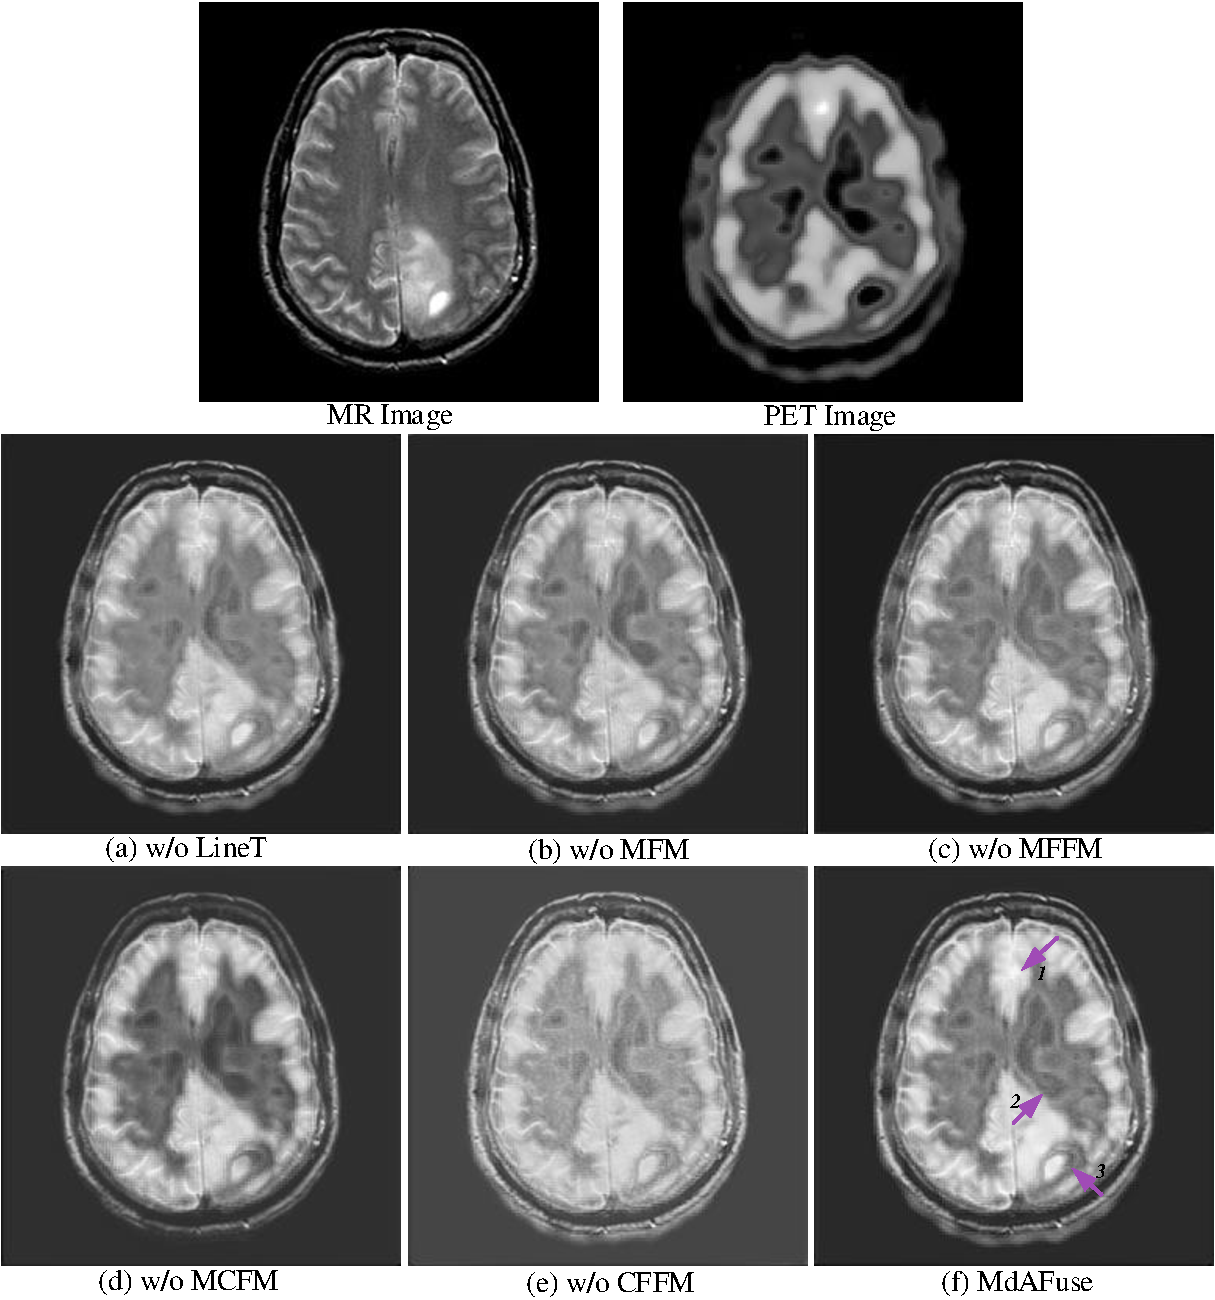
\includegraphics[width=0.85\columnwidth]{figs/paper2ablation1.pdf}
      \caption{本节所提出的影像融合方法的消融实验}\label{paper2ablation}
    \end{figure}

\subsubsection{脑影像的关键特征增强实验}
图\ref{paper2029_color_i}中的前两行显示了在五个周期内从具有脑异常的同一病例中采样的MRI-SPECT源影像。SPECT影像第二行的白色和黑色变化可用于确定病变的位置和病变的严重程度,有助于肿瘤的定位、分割和辅助诊断。第三行是前两行对应的MRI-SPECT影像对的融合结果,代表本节提出的方法的着色效果。从左到右的每列表示不同时间的成像结果。从图\ref{paper2029_color_i}中可以发现SPECT中能量信息的变化和容易判断异常的关键位置,主要体现在黄色轮廓和紫色区域。从左到右,融合结果上的黄色区域数量增加,左下顶叶的黄色区域增加,白色区域的亮度也提高。如果这种亮度代表较高的葡萄糖能量,则很可能在该位置发生糖尿病和高血糖。对于有黑点的区域,黑色块的数量随时间减少,但面积和浓度增加。例如,侧脑室枕角在图\ref{paper2029_color_i}(a)中只有一个小点,在图\ref{paper2029_color_i}(b)中形成两个小的蓝黑色区域。图\ref{paper2029_color_i}(c)中的黑蓝色区域的面积变大并向下移动,而图\ref{paper2029_color_i}(d)中的两个小区域合并,最后在图\ref{paper2029_color_i}(e)中面积扩大。表明该区存在异常。如果彩色区域代表细胞代谢能力,那么葡萄糖和蛋白质的严重缺乏可能会引起侧脑室枕角相应的疾病。因此,对融合结果进行着色可以增强融合后的效果,不仅可以揭示异常组织结构位置,还可以揭示能量变化,有助于准确诊断疾病演变。

\subsubsection{影像融合的消融实验}
为了充分说明浅层特征提取、深层特征提取、多尺度特征提取和线性变换融合策略的必要性和有效性,本节进行了五组消融实验,结果如图\ref{paper2ablation}所示。图\ref{paper2ablation}中的第一行表示一对多模态(MRI-PET)影像,第二至第三行展示出缺失线性变换操作的融合结果(w/o LinearT)、缺失多尺度特征提取模块(w/o MFM)、缺失多尺度和深层特征提取模块(w/o MFFM)、缺失多尺度和浅层特征提取模块(w/o MCFM)、缺失浅层和深层特征提取模块(w/o CFFM)以及所提方法的融合策略。在图\ref{paper2ablation}(f)中,三个箭头包含不同结果中的不同信息。在区域1中,应保留PET上的亮度信息。在图\ref{paper2ablation}(b)和图\ref{paper2ablation}(c)中,该位置的亮度不明显。在图\ref{paper2ablation}(a)和图\ref{paper2ablation}(d)中,位置模糊,这可能是由低亮度强度引起的。区域2是PET影像中的黑色区域,并且在MRI中灰度不均匀。在图\ref{paper2ablation}(b)和图\ref{paper2ablation}(d)中,它是具有均匀灰度级的区域。在图\ref{paper2ablation}(a)和图\ref{paper2ablation}(c)中,灰度级以特定梯度布置,但是边缘出现平滑现象。在图\ref{paper2ablation}(f)中,效果更好,并且保留了更多的结构信息。MRI上箭头3所指的区域是一个比扁豆大的小区域,亮度强而均匀,与周围的色差有层次关系。在这六种情况下,本节的MdAFuse方法都能反映出该位置的增强效果,取得了较好的效果。

  \begin{figure}[htbp]
      \centering
      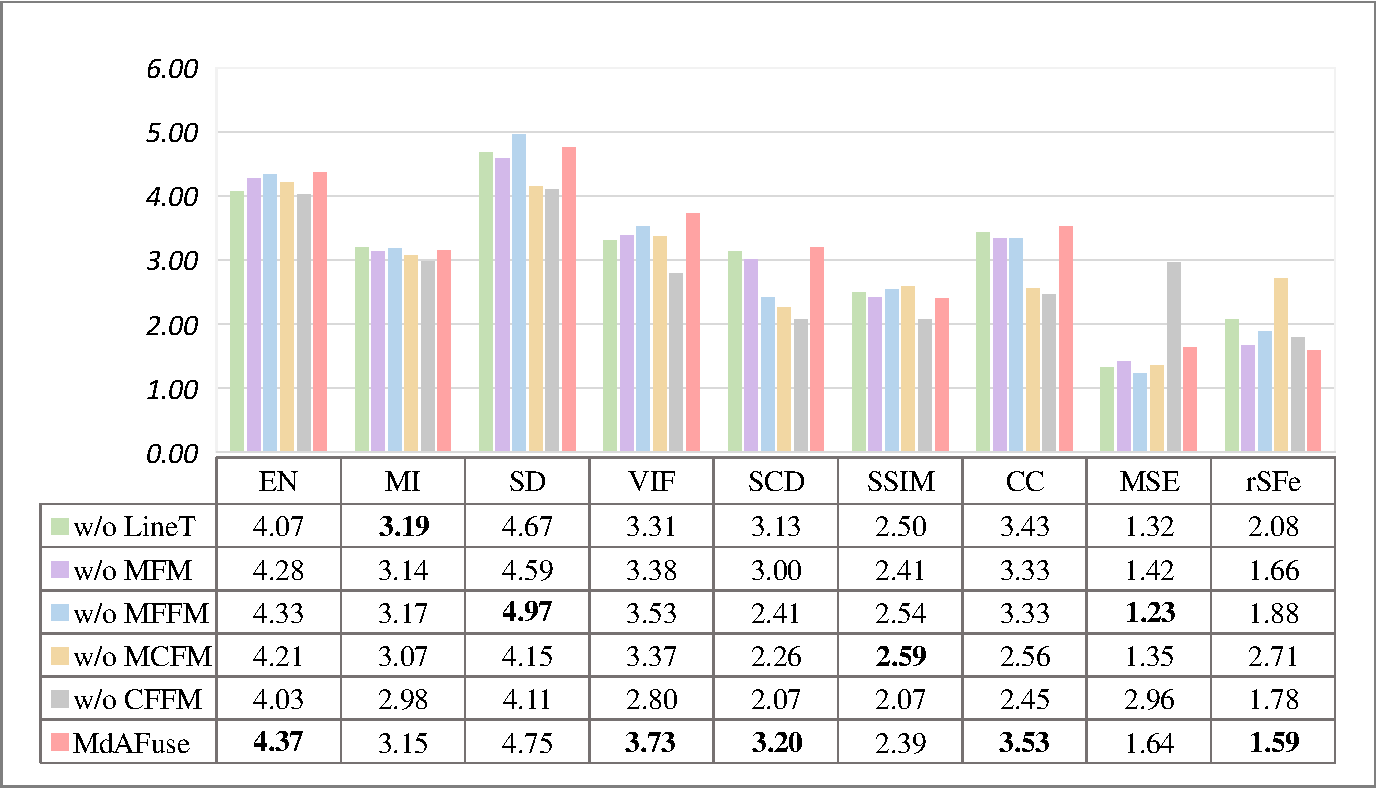
\includegraphics[width=0.9\columnwidth]{figs/paper2ablation2024_value1.pdf}
      \caption{消融实验结果(图\ref{paper2ablation})的9种质量评价指标显示}\label{paper2ablation_value1}
    \end{figure}
    
图\ref{paper2ablation_value1}显示了一些用于质量评估的指标值。在图\ref{paper2ablation_value1}中,下半部分是原始的六个度量值,上半部分是条形图显示。为了更好地观察和比较同一图表中不同的度量值,对每个度量值进行了线性变换,变换系数如表\ref{lineTransformation}所示。在图\ref{paper2ablation_value1}中,可以观察到本节的方法在5个指标中具有最优值,在1个指标中具有次优值。因此,相比较而言,本节提出的方法表现出了最佳的性能。因此,也说明了本节提出的MdAFuse方法对于其他融合方法在9种客观评估指标上的结果是最好的,这也证明了通过增加多维特征并使用自适应融合策略构建的网络可以获得更好的融合结果。
    

\subsection{小结}
在这小节中,本节提出了一种新的基于DL的融合框架,结合空间特征和通道特征的多维特征。同时,采用深度分离卷积网络,挖掘更丰富的有用信息,可为源影像提供显著特征和丰富细节特征,供后续影像理解和应用分析。采用三种不同的特征提取模块和一种基于各维特征相关性的自适应线性融合机制来保留MRI的空间纹理信息和PET/SPECT影像的生理代谢信息。此外,本节还提出了一种关键特征增强方法,该方法可以增强同一病例不同时期融合影像的可视化效果,有助于肿瘤定位、分割和疾病跟踪等临床应用。不同的疾病采用不同的常用影像学检查进行评价,多模态医学影像融合也是多种多样的。后续工作将持续研究不同类型的医学融合方法,并将其应用于人工智能医学诊断。

虽然本节的方法在MRI-PET/SPECT影像融合中表现出了一定的优势,但仍然存在一些局限性。本节的方法只关注MRI和PET/SPECT影像的关键特征,而不考虑某种疾病的特异性。此外,对于大脑影像的融合,没有增加对潜在疾病区域的神经科学分析。将联合神经科学与人工智能方法更深入地结合将是今后研究的一个有意义的方向。


\section{本章小结}
在\ref{chapter3.1:MsgFusion}节中,本节介绍了一种基于MS-Info引导的脑部疾病影像深度特征融合方法,被称为MsgFusion。该方法通过分析MRI/CT/PET/SPECT的关键MS-Info,获取相应的影像特征,并设计了一个包括SF-Branch和GV-Branch的双分支网络。SF-Branch结合了空间域和频域信息,GV-Branch结合了HSV颜色空间的多尺度灰度影像和亮度。这一双网络机制成功提高了CNN的泛化能力,充分考虑了频域信息和颜色空间信息的重要性,确保了融合结果的有效性。实验证明,在医学脑影像的处理和分析中,包括MRI-CT影像融合、MRI-SPECT影像融合和MRI-PET影像融合等方面,该方法相较于现有方法具有显著优势。通过临床医生的问卷调查评估和统计数据的支持,MsgFusion的融合效果被证实为最佳。

在\ref{chapter3.2:MdAFuse}小节中,本节提出了一种新的基于DL的融合框架,被称为MdAFuse,采用了空间特征和通道特征的多维度结合。引入深度分离卷积网络,旨在挖掘更丰富的有用信息,为源影像提供显著特征和丰富细节特征,以支持后续影像理解和应用分析。提出了三种不同的特征提取模块和一种基于各维特征相关性的自适应线性融合机制,以同时保留MRI的空间纹理信息和PET影像的生理代谢信息。此外,本节提出了一种关键特征增强方法,可提升同一病例不同时期融合影像的可视化效果,有助于肿瘤定位、分割和疾病跟踪等临床应用。考虑到不同疾病使用不同常用影像学检查进行评价,未来将持续研究和拓展多模态医学影像融合方法,以适应人工智能医学诊断的不断发展。
尽管本节的方法在MRI-PET/SPECT影像融合中表现出一定的优势,但仍存在一些局限性。本节的方法侧重于提取MRI和PET/SPECT影像的关键特征,而未考虑某种疾病的特异性。此外,在大脑影像的融合中,本节未加入对潜在疾病区域的神经科学分析。

未来,计划扩展框架,将两种以上的医学影像进行融合,并应用于更广泛的临床诊断场景。另外,将更深入地探讨如何将神经科学与人工智能方法更加紧密地结合,以实现更全面和准确的医学影像融合。

%%% Local Variables:
%%% mode: latex
%%% TeX-master: "../main"
%%% End:
|
\item 在47-63行的位置, 仿照其他语句加入\verb|chapter/chapter3,|(注意后面有个英文的逗号)
\item 打开chapter3.tex, 第1行输入内容
\begin{verbatim}
% !TEX root = ../main.tex
\end{verbatim}
从第2行开始输入正文.
\item 编译查看结果.
\end{enumerate}

Q2: 如何修改论文作者信息?\\
A2: 直接修改cover.cfg文件中的信息.\\

Q3: 如何加入自定义命令和宏包?\\
A3: 请在defcommands.tex中添加自定义命令和宏包.\\

Q4: 可否修改为硕士学位论文?\\
A4: 本模板默认为博士学位论文. 若要修改为硕士论文, 请在main.tex文件中将语句\verb|\phdtrue|注释掉, 同时取消\verb|\phdfalse|的注释. (目前仍有BUG待解决, 例如偶数页页眉, 最后发表的文章和项目部分仍显示博士)\\

Q5: 如何生成盲审论文?\\
A5: 首先确保main.tex文件中的第48行这个\verb|\includeonly|命令中正确包含了需要盲审的章节, 然后按如下步骤操作:
\begin{enumerate}
\item 在main.tex文件中注释掉\verb|\blindfalse|, 打开\verb|\blindtrue|
\item 取消\verb|\linenumbers|的注释, 正文部分每隔5行自动生成一个行号
\item 使用xelatex编译3次生成盲审结果
\end{enumerate}

Q6: 能否生成不同版本号用来区分不同的版本?\\
A6: 打开cover.cfg, 在\verb|\version{}|中填写需要的版本号, 如此, 将在首页生成一个版本号信息. 本模板提供了自定义了一个日期时间作为版本号, 调用方式为输入\verb|\version{\today}|, 结果如同(版本: \today). 当然, 版本号可以修改为任意其他文字, 例如定稿时, 修改为``终稿''.
